\documentclass{book}

\title{Certified Security by Design Applied to the Patrol Based\\
  A Demonstration of CSBD Applicability to Military Operations}
\author{Professor Shiu-Kai Chin, Lori Pickering, Jesse Nathanial Hall, YiHong Guo}
\date{August 2017}

\usepackage{634format}
\usepackage{enumerate}
\usepackage{listings}
\usepackage{textcomp}
\usepackage{amsmath}
\usepackage{hyperref}
\usepackage{holtex}
\usepackage{holtexbasic}
\usepackage{subfiles}
\usepackage{array}
\usepackage{pdflscape}
\usepackage{textcomp}
\usepackage{multirow}
\usepackage[table]{xcolor}
%\usepackage[usenames, dvipsnames]{color}
\usepackage{graphicx}
\usepackage{color}
\graphicspath{ {diagrams/}{pictures/}{MethodsAP/picture/}{appendix/pictures/} }
% =====================================================================
%
% Macros for typesetting the HOL system manual
%
% =====================================================================

% ---------------------------------------------------------------------
% Abbreviations for words and phrases
% ---------------------------------------------------------------------

\newcommand\TUTORIAL{{\footnotesize\sl TUTORIAL}}
\newcommand\DESCRIPTION{{\footnotesize\sl DESCRIPTION}}
\newcommand\REFERENCE{{\footnotesize\sl REFERENCE}}
\newcommand\LOGIC{{\footnotesize\sl LOGIC}}
\newcommand\LIBRARIES{{\footnotesize\sl LIBRARIES}}
\usepackage{textcomp}

\newcommand{\bs}{\texttt{\char'134}} % backslash
\newcommand{\lb}{\texttt{\char'173}} % left brace
\newcommand{\rb}{\texttt{\char'175}} % right brace
\newcommand{\td}{\texttt{\char'176}} % tilde
\newcommand{\lt}{\texttt{\char'74}} % less than
\newcommand{\gt}{\texttt{\char'76}} % greater than
\newcommand{\dol}{\texttt{\char'44}} % dollar
\newcommand{\pipe}{\texttt{\char'174}}
\newcommand{\apost}{\texttt{\textquotesingle}}
% double back quotes ``
\newcommand{\dq}{\texttt{\char'140\char'140}}
%These macros were included by slind:

\newcommand{\holquote}[1]{\dq#1\dq}

\def\HOL{\textsc{Hol}}
\def\holn{\HOL}  % i.e. hol n(inety-eight), no digits in
                 % macro names is a bit of a pain; deciding to do away
                 % with hol98 nomenclature means that we just want to
                 % write HOL for hol98.
\def\holnversion{Kananaskis-11}
\def\holnsversion{Kananaskis~11} % version with space rather than hyphen
\def\LCF{{\small LCF}}
\def\LCFLSM{{\small LCF{\kern-.2em}{\normalsize\_}{\kern0.1em}LSM}}
\def\PPL{{\small PP}{\kern-.095em}$\lambda$}
\def\PPLAMBDA{{\small PPLAMBDA}}
\def\ML{{\small ML}}
\def\holmake{\texttt{Holmake}}

\newcommand\ie{\mbox{\textit{i{.}e{.}}}}
\newcommand\eg{\mbox{\textit{e{.}g{.}}}}
\newcommand\viz{\mbox{viz{.}}}
\newcommand\adhoc{\mbox{\it ad hoc}}
\newcommand\etal{{\it et al.\/}}
% NOTE: \etc produces wrong spacing if used between sentences, that is
% like here \etc End such sentences with non-macro etc.
\newcommand\etc{\mbox{\textit{etc{.}}}}

% ---------------------------------------------------------------------
% Simple abbreviations and macros for mathematical typesetting
% ---------------------------------------------------------------------

\newcommand\fun{{\to}}
\newcommand\prd{{\times}}

\newcommand\conj{\ \wedge\ }
\newcommand\disj{\ \vee\ }
\newcommand\imp{ \Rightarrow }
\newcommand\eqv{\ \equiv\ }
\newcommand\cond{\rightarrow}
\newcommand\vbar{\mid}
\newcommand\turn{\ \vdash\ } % FIXME: "\ " results in extra space
\newcommand\hilbert{\varepsilon}
\newcommand\eqdef{\ \equiv\ }

\newcommand\natnums{\mbox{${\sf N}\!\!\!\!{\sf N}$}}
\newcommand\bools{\mbox{${\sf T}\!\!\!\!{\sf T}$}}

\newcommand\p{$\prime$}
\newcommand\f{$\forall$\ }
\newcommand\e{$\exists$\ }

\newcommand\orr{$\vee$\ }
\newcommand\negg{$\neg$\ }

\newcommand\arrr{$\rightarrow$}
\newcommand\hex{$\sharp $}

\newcommand{\uquant}[1]{\forall #1.\ }
\newcommand{\equant}[1]{\exists #1.\ }
\newcommand{\hquant}[1]{\hilbert #1.\ }
\newcommand{\iquant}[1]{\exists ! #1.\ }
\newcommand{\lquant}[1]{\lambda #1.\ }

\newcommand{\leave}[1]{\\[#1]\noindent}
\newcommand\entails{\mbox{\rule{.3mm}{4mm}\rule[2mm]{.2in}{.3mm}}}

% ---------------------------------------------------------------------
% Font-changing commands
% ---------------------------------------------------------------------

\newcommand{\theory}[1]{\hbox{{\small\tt #1}}}
\newcommand{\theoryimp}[1]{\texttt{#1}}

\newcommand{\con}[1]{{\sf #1}}
\newcommand{\rul}[1]{{\tt #1}}
\newcommand{\ty}[1]{\textsl{#1}}

\newcommand{\ml}[1]{\mbox{{\def\_{\char'137}\texttt{#1}}}}
\newcommand{\holtxt}[1]{\ml{#1}}
\newcommand\ms{\tt}
\newcommand{\s}[1]{{\small #1}}

\newcommand{\pin}[1]{{\bf #1}}
% FIXME: for multichar symbols \mathit should be used.
\def\m#1{\mbox{\normalsize$#1$}}

% ---------------------------------------------------------------------
% Abbreviations for particular mathematical constants etc.
% ---------------------------------------------------------------------

\newcommand\T{\con{T}}
\newcommand\F{\con{F}}
\newcommand\OneOne{\con{One\_One}}
\newcommand\OntoSubset{\con{Onto\_Subset}}
\newcommand\Onto{\con{Onto}}
\newcommand\TyDef{\con{Type\_Definition}}
\newcommand\Inv{\con{Inv}}
\newcommand\com{\con{o}}
\newcommand\Id{\con{I}}
\newcommand\MkPair{\con{Mk\_Pair}}
\newcommand\IsPair{\con{Is\_Pair}}
\newcommand\Fst{\con{Fst}}
\newcommand\Snd{\con{Snd}}
\newcommand\Suc{\con{Suc}}
\newcommand\Nil{\con{Nil}}
\newcommand\Cons{\con{Cons}}
\newcommand\Hd{\con{Hd}}
\newcommand\Tl{\con{Tl}}
\newcommand\Null{\con{Null}}
\newcommand\ListPrimRec{\con{List\_Prim\_Rec}}


\newcommand\SimpRec{\con{Simp\_Rec}}
\newcommand\SimpRecRel{\con{Simp\_Rec\_Rel}}
\newcommand\SimpRecFun{\con{Simp\_Rec\_Fun}}
\newcommand\PrimRec{\con{Prim\_Rec}}
\newcommand\PrimRecRel{\con{Prim\_Rec\_Rel}}
\newcommand\PrimRecFun{\con{Prim\_Rec\_Fun}}

\newcommand\bool{\ty{bool}}
\newcommand\num{\ty{num}}
\newcommand\ind{\ty{ind}}
\newcommand\lst{\ty{list}}

% ---------------------------------------------------------------------
% \minipagewidth = \textwidth minus 1.02 em
% ---------------------------------------------------------------------

\newlength{\minipagewidth}
\setlength{\minipagewidth}{\textwidth}
\addtolength{\minipagewidth}{-1.02em}

% ---------------------------------------------------------------------
% Environment for the items on the title page of a case study
% ---------------------------------------------------------------------

\newenvironment{inset}[1]{\noindent{\large\bf #1}\begin{list}%
{}{\setlength{\leftmargin}{\parindent}%
\setlength{\topsep}{-.1in}}\item }{\end{list}\vskip .4in}

% ---------------------------------------------------------------------
% Macros for little HOL sessions displayed in boxes.
%
% Usage: (1) \setcounter{sessioncount}{1} resets the session counter
%
%        (2) \begin{session}\begin{verbatim}
%             .
%              < lines from hol session >
%             .
%            \end{verbatim}\end{session}
%
%            typesets the session in a numbered box.
% ---------------------------------------------------------------------

\newlength{\hsbw}
\setlength{\hsbw}{\textwidth}
\addtolength{\hsbw}{-\arrayrulewidth}
\addtolength{\hsbw}{-\tabcolsep}
\newcommand\HOLSpacing{13pt}

\newcounter{sessioncount}
\setcounter{sessioncount}{0}

\newenvironment{session}{\begin{flushleft}
 \refstepcounter{sessioncount}
 \begin{tabular}{@{}|c@{}|@{}}\hline
 \begin{minipage}[b]{\hsbw}
 \vspace*{-.5pt}
 \begin{flushright}
 \rule{0.01in}{.15in}\rule{0.3in}{0.01in}\hspace{-0.35in}
 \raisebox{0.04in}{\makebox[0.3in][c]{\footnotesize\sl \thesessioncount}}
 \end{flushright}
 \vspace*{-.55in}
 \begingroup\small\baselineskip\HOLSpacing}{\endgroup\end{minipage}\\ \hline
 \end{tabular}
 \end{flushleft}}

% ---------------------------------------------------------------------
% Macro for boxed ML functions, etc.
%
% Usage: (1) \begin{holboxed}\begin{verbatim}
%               .
%               < lines giving names and types of mk functions >
%               .
%            \end{verbatim}\end{holboxed}
%
%            typesets the given lines in a box.
%
%            Conventions: lines are left-aligned under the "g" of begin,
%            and used to highlight primary reference for the ml function(s)
%            that appear in the box.
% ---------------------------------------------------------------------

\newenvironment{holboxed}{\begin{flushleft}
  \begin{tabular}{@{}|c@{}|@{}}\hline
  \begin{minipage}[b]{\hsbw}
% \vspace*{-.55in}
  \vspace*{.06in}
  \begingroup\small\baselineskip\HOLSpacing}{\endgroup\end{minipage}\\ \hline
  \end{tabular}
  \end{flushleft}}

% ---------------------------------------------------------------------
% Macro for unboxed ML functions, etc.
%
% Usage: (1) \begin{hol}\begin{verbatim}
%               .
%               < lines giving names and types of mk functions >
%               .
%            \end{verbatim}\end{hol}
%
%            typesets the given lines exactly like {boxed}, except there's
%            no box.
%
%            Conventions: lines are left-aligned under the "g" of begin,
%            and used to display ML code in verbatim, left aligned.
% ---------------------------------------------------------------------

\newenvironment{hol}{\begin{flushleft}
 \begin{tabular}{c@{}@{}}
 \begin{minipage}[b]{\hsbw}
% \vspace*{-.55in}
 \vspace*{.06in}
 \begingroup\small\baselineskip\HOLSpacing}{\endgroup\end{minipage}\\
 \end{tabular}
 \end{flushleft}}

% ---------------------------------------------------------------------
% Emphatic brackets
% ---------------------------------------------------------------------

\newcommand\leb{\lbrack\!\lbrack}
\newcommand\reb{\rbrack\!\rbrack}


% ---------------------------------------------------------------------
% Quotations
% ---------------------------------------------------------------------


%These macros were included by ap; they are used in Chapters 9 and 10
%of the HOL DESCRIPTION

\newcommand{\inds}%standard infinite set
 {\mbox{\rm I}}

\newcommand{\ch}%standard choice function
 {\mbox{\rm ch}}

\newcommand{\den}[1]%denotational brackets
 {[\![#1]\!]}

\newcommand{\two}%standard 2-element set
 {\mbox{\rm 2}}


\begin{document}
\lstset{language=ML}
\maketitle{}

\tableofcontents{}

\addcontentsline{toc}{chapter}{List of Figures}
\listoffigures

\addcontentsline{toc}{chapter}{Preface}
\chapter*{Preface}
\label{cha:preface}
This documentation describes the research methods, results, future work, and conclusions
for the proof of concept project discussed herein.   The Introduction briefly describes
the purpose of the project.  The Methods, Assumptions, and Procedures  section follows.
It describes the basic concepts of applying the principle of complete mediation to the
patrol base operations using a hierarchy of \emph{secure} state machines.  It also describes the
technologies employed for the project.  Following the Methods, Assumptions, and Procedures
section is the Results  section.   This section is divided into three parts.  The first
part describes the folders and files and the folder structure for the project.  It is intended
to aid the reader in finding files and folders in the project. The next section details the
ACL and HOL verification of the project.  It details the datatypes, definitions, and theorems
used in verifying the hierarchy of \emph{secure} state machines.  In this section, the code and its
purpose are discussed.  Examples of code are also included.  The third section describes the
results of translating the patrol base operations into a hierarchy of \emph{secure} state machines.
The logic and rationale for the structure are described .   The Future Work and Research
section describes works that were discussed but not verified in the ACL and HOL.  It also
hints on how this project may be employed in future automations of the patrol base operations.
The Conclusion wraps everything up.\\

Other sections support this documentation.  This includes a list of figures and acronyms.
In addition, the appendix contains the full EmitTeX pretty-printed datatypes, definitions,
and theories generated in the project.  The actual HOL code (not so pretty-printed form) and
the diagrams for the hierarch of \emph{secure} state machines are also included in the appendix.

\addcontentsline{toc}{chapter}{Acknowledgments}
\chapter*{Acknowledgments}
\label{cha:acknowledgments}
  This project involved multiple people at multiple levels. The Principal Investigator was
  Professor Shiu-Kai Chin of Syracuse University’s Department of Engineering and Computer Science.
  Lori Pickering, Graduate Student at Syracuse University’s Department of Engineering and Computer
  Science, primarily worked on the access-control logic (ACL) and higher order logic (HOL)
  implementation of the patrol base. Together with Jesse Nathanial Hall, they constructed the
  idea of translating the patrol base operations into state machines. Jesse, also a student at
  Syracuse University in the iSchool and a [rank] in the U.S. Army, was our subject matter expert.
  Once Jesse and Lori decided on the state machine format, Jesse translated the patrol base operations
  into this format. YiHong Guo came to the project near the end. Nevertheless, he contributed significantly
  to the project. YiHong worked on organizing the documentation in LaTeX.


\chapter{Summary}
\label{cha:summary}


\chapter{Introduction}
\label{cha:introduction}
Platoon patrol base (PB) operations are an essential part of many military operations.
They provide Soldiers with a means to avoid enemy contact, rest, resupply, and conduct Squad
level missions (Ranger Handbook 2011, 132). Although some might believe that a PB begins from
an objective rally point (ORP), a PB must be planned for. Our PB software includes a state
machine model for tasks that include planning, movement, as well as conducting both an ORP and PB.\\

Any automation of the patrol base operations (for example Jesse? Professor Chin?) would require
that the design of such system be certified as secure from the start. This approach should be
applied to all systems. Yet, our aim in this project was to show that the certified security by
design approach could be applied specifically to the patrol base operations because it is described
in a manner that is similar to many other military operations. These operations will, no doubt,
be automated in the future. Thus, this project should be viewed as a primer on how to tackle such
an automation in a secure manner, from the start.\\

The certified security by design approach involves taking the design of the automated system and
using access-control logic (ACL) to prove that any action that takes place in the automated system
is correctly executed and has the appropriate authorizations and authentications of those authorities.
Computer-aided reasoning is used to verify that the system is secure. For this project, we used the
higher order logic (HOL) theorem prover. HOL is a trusted and reliable system. It is commonly said by
the HOL community that “HOL is never wrong.”\\

The access-control logic (ACL) was developed by Professor Shiu-Kai Chin and Professor Susan Older of
Syracuse University’s Department of Engineering and Computer Science. Specifics can be found in their
text book titled Access Control, Security, and Trust. The definitions and theorems from the text were
implemented in HOL by Professor Shiu-Kai Chin and Lockwood Morris. For reference a report of the datatypes,
definitions, and theorems that were implemented in HOL are provided in Appendices ?\\

Our method for understanding what represented mission failure and mission success was guided by Functional
Mission Analysis (Young,…?). We identified that our goal was to develop “A system to provide mission
assurance for execution of patrol base operations by means of logical proof in order to mitigate
enemy/civilian contact and mission failure.” Unacceptable losses would normally be at the Higher
Headquarter (HHQs) Commander’s discretion, but for the sake of our project they were the (L1) loss
of civilian life, (L2) 20\% of our Platoon being rendered Non-Mission Capable (NMC), and (L3) mission
failure. Hazards that could lead to unacceptable losses included (H1) contact with civilians, (H2)
contact with the enemy, and (H2) loss of adequate mission essential supplies. The table below
illustrated our causal links between hazards and losses.\\

\begin{figure}[h]               
  \centering
  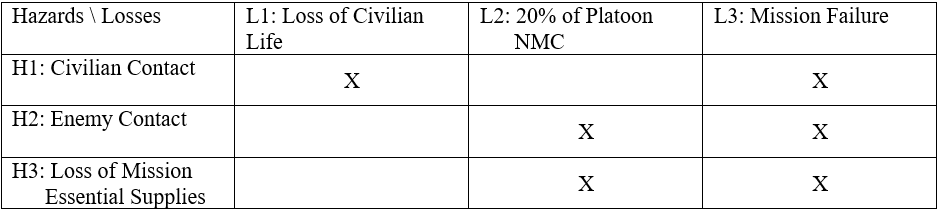
\includegraphics[scale=0.46]{HazardChart.PNG}
  \caption{Hazard or Loss Table}
\end{figure}

Our functional control structure is the chain of command illustrated below outlines what individual,
in what unit level would be responsible for the actions of the Soldiers below them.\\

\begin{figure}[h]
  \centering
  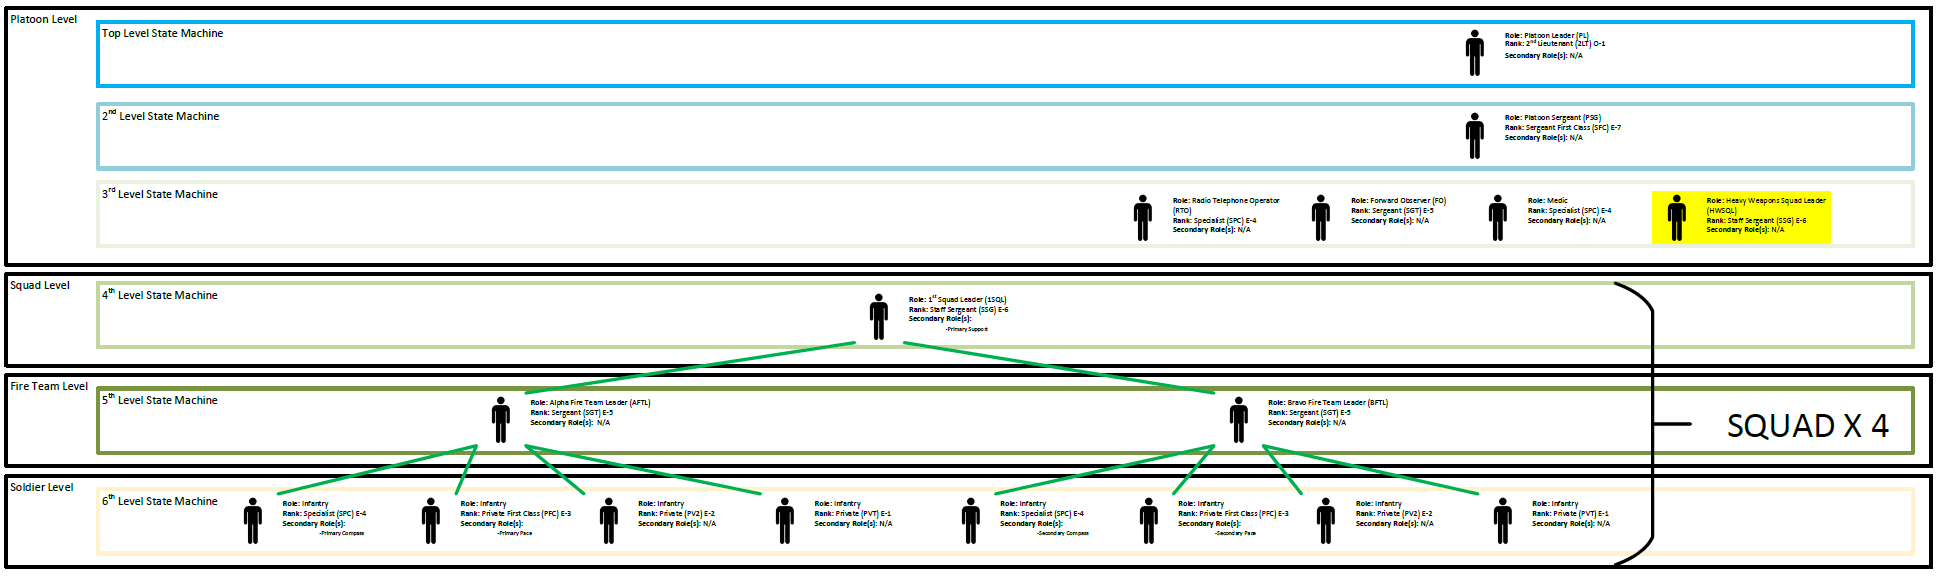
\includegraphics[scale=0.3]{OrganizationalChart.png}
  \caption{Organizational Chart}
\end{figure}

The organizational chart showed the hierarchy of the Platoon and whom would be in control of
each element and responsible for mitigating risks caused by hazards. Our application design
recognized each leaders’ ability to control certain groups/units of Soldiers. With this in
mind, leaders within the Platoon would have to (C1) avoid populated areas, (C2) avoid trafficked
routes to and from those areas, (C3) maintain supplies within the HHQ standard operating
procedure (SOP). These constraints were built into our application with states that performed
reconnaissance, uniform and packing list checks, maintenance and cross loading of supplies.\\

% ---- this points LaTeX to PatrolBaseDoc.tex ----
% Local Variables:
% TeX-master: "../PatrolBaseDoc"
% End:

\chapter{Methods, Assumptions, and Procedures}
\label{cha:meth-assumpt-proc}
% \section{Methods}
% \label{sec:methods}

\chapter{Methods}
\label{cha:methods}
\ \ \ \ The doctrine reflected in our project was taken from the Ranger Handbook
(Ranger Handbook 2011). Our first task was to reflect a patrol base (PB)
in two-dimensional form so that we could analyze possible courses of action
with regard to modularizing and parameterizing PB operations. Microsoft\textregistered
Powerpoint was used for the initial sketches, which provided a visual
reference for the entire PB from planning through actual withdrawal from
the PB (see figure 3.1). The reasoning behind inclusion of a planning state
was that our entire project was based on ensuring the proper execution of
a PB, and proper execution begins with planning.\ \\\\

\begin{figure}[h]
  \centering
  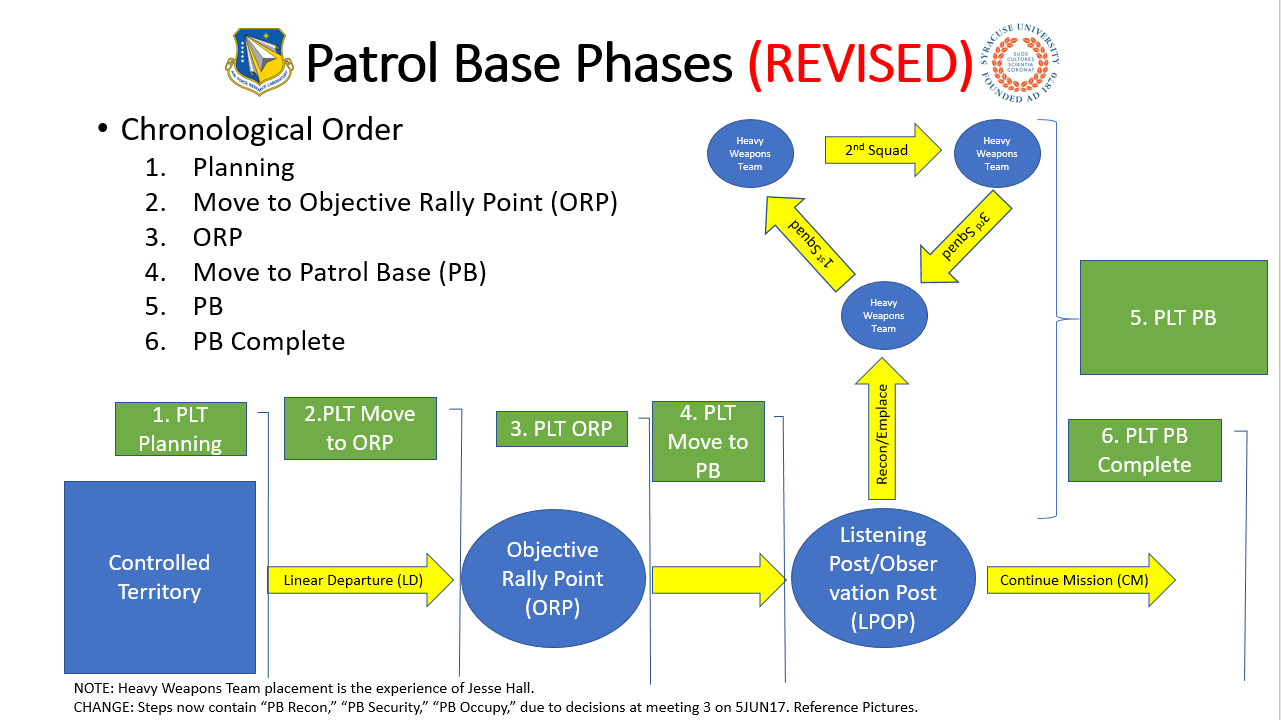
\includegraphics[width=0.7\linewidth]{map31.png}
  \caption{PB Phase Overview}
\end{figure}
After the PB was broken into phases, we began creating states that mimicked
the phases outlined in the Powerpoint\textcopyright document (figure 3.1). Microsoft\textregistered
Visio was used to illustrate the states, their order, and the commands that
initiated movement from one state to another (figure 3.2). The decision to
adopt a state machine as the method for rendering PB operations came from
previous projects Dr. Shiu-Kai Chin had allowed our team to review. Projects
programmed in Poly Meta Language (Poly/ML) and compiled with High Order
Logic (HOL) seemed to lend themselves well to the state machine structure.\\ \\

% \subsection{The Implementation Approach}
% \label{sec:impl-appr-1}

\section{The Implementation Approach}
\label{sec:impl-appr}

The goal was to represent the patrol base in a way that would be amiable to applying access-control
logic (ACL) principles. The motive for this project was, in fact, to demonstrate the applicability
of these principles to the mission assurance objective. Representing the patrol base in terms of
state machines was easily implemented with computer-aided reasoning, in this case the HOL higher
order logic theorem prover. The basic idea was to establish states, commands to transition from one
state to another, and people who were authorized to make these commands. To do this, it was first
necessary to translate the patrol base into discrete states. This was where the subject matter
expertise of Jesse was crucial. The details were described in the section “add section title here.”

% \subsection{Hierarchy of State Machines}
% \label{sec:hier-state-mach-1}

\section{Hierarchy of State Machines}
\label{sec:hier-state-mach}

In this project, we decided on a hierarchy of state machines with a top-level state machine,
sub-level state machines, and sub-sub-level state machines, etc. as the foundational approach.
That is, we began with a top-level state machine consisting of 6 states. Each state (save for the
terminal state) was yet another state machine at a sub-level. We called this a sub-level state machine.
There was one sub-level state machine for each state in the top-level state machine. This produced at
pyramid-like, top down structure. Adding yet another level, the sub-sub-level, produced a state
machine for each state machine in the higher-up sub-level state machine. These were called the sub-sub-
level state machines. Beyond this level, we considered alternative approaches. Although we discussed
and worked out some strategies here, the project was simply too large for one summer. These ideas are
discussed in the “Future Work” section.

The reason for this pyramid-like approach was multi-fold.
\begin{itemize}
\item First, it was logical to look at the patrol base as a whole and design a basic,
  top-level state machine that represented the most basic states. Going into too much
  detail at first would be distracting and thus error-prone.
\item Second, this approach facilitated a test of the state machine approach before
  going into too much depth. It was easy to see at the top-level what would work and
  what would not work.
\item Third, it allowed for separation of tasks. Jesse’s expertise was in his knowledge
  of the patrol base and his ability to work with Visio and other similar technologies.
  Lori’s expertise was in her knowledge of the access-control logic (ACL) principles and
  her ability to work with the higher order logic (HOL) theorem prover. Once a top-level
  state machine was established, Jesse continued work on the delineation of the patrol base
  into state machines while Lori began work on implementing the state machine(s) using the
  ACL principals and HOL.
\item Fourth, the modularization facilitated the concept of separation of implementation.
  For example, if someone were to take the top-level state machine and delegate the sub-level
  state machines to others, then they could all be integrated together at a later time. The
  same could be said at the sub-level, and so on. The idea of integration is discussed further
  in the “Future Works” section.
\item Fifth, approaching the project one level at a time facilitated a step-by-step approach
  to solving each new level of complexity while capitalizing on previous successes. Because of
  the nature of HOL, once we solved one problem in the implementation of the patrol base, we could
  rely on that solution. The next problem could then be isolated and attacked without back-tracking—
  for the most part. We could add complexity as we approached it, in analogy to the complexity of
  detail in the patrol base itself.
\item Sixth, time constraints on the project were tight. As we delved into the sub-level
  and sub-sub-level state machines, the level of detail that needed to be implemented in the
  ACL and HOL became apparent. The outlooks for the project were exciting. And, at the same time,
  we realized that a complete implementation of the patrol base in HOL would require more than one
  summer. Thus, the level-by-level approach facilitated a view of what could be done based on
  what had been done, demonstrating the practicality of the application of ACL and HOL to a patrol
  base-like problem. This was our goal.
\end{itemize}

% \subsection{The Secure State Machine}
% \label{sec:secure-state-machine-2}

\section{The Secure State Machine}
\label{sec:secure-state-machine}

Again, the reason for the state machine approach was that it was the simplest
way to represent a large project using ACL and implement it using HOL. If the
patrol base was represented as a state machine, then the orders/commands could
be represented as inputs into the states. This was what we did. We determined
at each level, what should be considered a state and what order/command should
be given to transition from that state to the next. For a basic state machine,
this was all that was needed to represent the given level of complexity.
However, in general, we were concerned with authentication and authorization.
Who was giving the command and did that person have the authority to give that
command? Thus, we needed the appropriate checks on identity (authentication)
and authority to make the transition from one state to another. We needed not
just a \textit{state machine} but a \textit{secure state machine}.\\

For a secure state machine, we hiked up the complexity of our state machine model.
We now only allowed a transition from one state to another if the order was given by
someone (or something) that was authenticated and authorized. We called that someone
(or something) in the access-control logic (ACL) a “principal.” For example, we
authenticate (via visual recognition) a soldier as the platoon leader. We establish
\textit{a priori} that the platoon leader had the authority to command a change from one
state to another. Given those conditions, we wanted our state machine to make that
change. More specifically, assume we were in the planning phase of the patrol base.
We called this the PLAN_PB state. (To be consistent we denoted all states by capital
letters.) In this state, the platoon leader said “cross the line of discrimination.”
We abbreviated this command as “crossLD”. (We used primarily lower-case letters for
commands.) Furthermore, we all knew that the platoon leader was authorized to give the
command to cross the line of discrimination and begin the next phase of the patrol base.
We called this next phase the MOVE_TO_ORP state. Under these circumstances, the access-
control logic dictated that we transition from the PLAN_PB state to the MOVE_TO_ORP state.
We did this for each state, using the ACL and HOL to verify the proper authentication and
authority for each transition. This was the security by design approach.

% \subsection{Authentication}
% \label{sec:authentication-1}

\section{Authentication}
\label{sec:authentication}

In the example above, the authentication of the principal (the platoon leader) was
assumed to be common knowledge. This was easy for soldiers who
could verify the identity of an individual via visual inspection or voice recognition.
In the world of computers and/or wherein an individual was not known (such as a
security gate check-point or a computer terminal), more formal methods of authentication
were required. Although time constraints did not allow us to consider that for this
project, the applicability of the secure state machine approach had already been
demonstrated elsewhere using cryptographic functions, key cards, etc. This was also
discussed in the “Future Work” section.\\

For the purposes of this project, the authenticated persons were listed in an \textit{authentication test
function}. This function was a list of the form:
\begin{itemize}
\item Platoon Leader says “someCommand” = true,
\item Platoon Sergeant says “someCommand” = true,
\item Anything else = false.
\end{itemize}

Additional principals could have been listed or deleted as needed by each secure
state machine. Two principals were the maximum needed to the extent to which this
project was implemented in HOL. Most states required only one principal, namely
the platoon leader. Each secure state machine had its own \textit{authentication test
function} with its own list of principals. In the implementation, if a principal
other than those listed in the \textit{authentication test function} were to make a request,
HOL would not allow the transition (or any other action) to occur.\\

The top-level state machine was implemented with only one principal, namely the
platoon leader. In other words, the platoon leader was responsible all that commands
in the top-level state machine. When the sub-level state machines were implemented,
two state machines included two principals each making commands, namely the platoon
leader and the platoon sergeant. This caused some issues with HOL because of the
nature of the biconditional. If an authenticated and authorized principal gives the
command to change states then we proved in HOL that the transition should occur.
On the converse, if the transition occurred then we also proved in HOL that an
authenticated and authorized principal must have made the command. But, what if there
were two authenticated and authorized principals? Which one made the command? The
problem wasn’t overly challenging; however, it did require a different strategy than
was used for the one principal secure state machines. The simplest approach was to
allow each principal to control a specific set of commands. Thus, there were platoon
leader commands and platoon sergeant commands. If a transition was made using a platoon
leader command, then the platoon leader must have made the command. The same was true
for the platoon sergeant. The biconditional problem was solved. Nevertheless, there
were several other strategies which were explored and could have been implemented in
other secure state machines to demonstrate the flexibility of HOL.

% \subsection{Authorization}
% \label{sec:authorization}

\section{Authorization}
\label{sec:authorization-1}

In the ACL secure state machine approach, authentication was governed by a list of
statements dictating who “controls” what and under what conditions that control was
governed. This was essentially a list of trust assumptions, certificates, authorities,
etc. For the level of complexity that was implemented in this project, access was
dictated by a prescribed \textit{security context list}, consisting of statements such as
“Platoon Leader \textbf{controls} crossLD”. In other words, this was the ACL representation
of the policy stating that “the Platoon Leader has the authority to execute the
command “’crossLD’.” Of course, representation of the statement in HOL was more complex.
Nevertheless, it amounted to just this declaration of authority.\\

An additional level of complexity was added to the \textit{security context} list of the ssmPlanPB
state machine. It was also planned for other state machines at the sub-sub-level. This was
necessary as the complexity of the project grew. In previously implemented secure state
machines in the project, transitions from one state to another were sequential. To get from
one state, the previous state must have been completed. For the ssmPlanPB state machine,
the transition from the WARNO state to the COMPLETE state was to occur after the middle three
states were completed. However, these states did not need to be completed in any order.
But, all three states \textit{had to be completed} before transitioning to the COMPLETE state. The
easiest implementation approach involved allowing a list of inputs to the state machine.
For example, the transition from WARNO to COMPLETE was to occur only if a list of requests/commands,
say [a,b,c], was given as input, where each letter represented a request (i.e., a = Platoon
Leader says “state a is complete”). The order of this list was irrelevant. There were thus six
permutations of the list that could be passed as input to the state machine. It worked.\\

Nevertheless, the use of lists and permutations was not the most elegant solution and could
cause problems in integrating state machines later on (see “future work”). Thus, a second version
of the ssmPlanPB state machine was generated and named testssmPlanPB. This used the approach described next.\\

Consider the case wherein the Platoon Leader (or other principal) had the authority to
execute a command if and only if some set of conditions were met. For example, a, b, and
c must have occur before the command could be executed. a, b, and c could have been the
following statements: Platoon Leader says “state 2 is complete”; Platoon Sergeant says
“state 3 is complete”; and Platoon Leader says “state 4 is complete”. Under those conditions,
we wanted the Platoon Leader to have the authority to execute a change of state from WARNO
to COMPLETE To do this in the ACL, a line in the \textit{security context} list would look like the following:
\begin{itemize}
\item Platoon Leader \textbf{says} “state 2 is complete” and
\item Platoon Sergeant \textbf{says} “state 3 is complete” and
\item Platoon Leader \textbf{says} “state 4 is complete” implies
\item Platoon leader \textbf{controls} “complete”.
\end{itemize}
Thus, when the Platoon Leader says “complete”, our theorem prover would check the \textit{security
context} list, check that all the conditions in the list were met, and then execute the transition
if and only if all conditions were met. This was the approach implemented in testssmPlanPB.\\

In addition, we knew because of the reliability of HOL that if the transition was executed, then
all of the said conditions above were met, namely.\\

\begin{itemize}
\item If we are now in the state COMPLETE, then it is also true that
\item Platoon Leader \textbf{says} “complete” is true (that is, the Platoon Leader made the request), and
\item Platoon Leader \textbf{says} “state 2 is complete” is true, and
\item Platoon Sergeant \textbf{says} “state 3 is complete” is true, and
  \item Platoon Leader \textbf{says} “state 4 is complete” is also true.
  \end{itemize}
  Other conditions could have been added and were discussed for future work.

% \subsection{State Interpretation}
% \label{sec:state-interpretation}

\section{State Interpretation}
\label{sec:state-interpretation-1}

In addition to authentications and authorizations, the behavior of the state machine could have
been controlled by the definitions that were state-dependents. This approach was briefly considered,
in particular for the two-principal problem discussed above. However, time constraints favored the
simpler approach discussed. Nevertheless, it was worth mentioning and could be explored if the project
were to be extended.

% \subsection{Implementation of the Secure State Machine Model}
% \label{sec:impl-secure-state}
\section{Implementation of the Secure State Machine Model}
\label{sec:impl-secure-state-1}


For reasons pertaining to simplicity and experience, Professor Shiu-Kai Chin’s model of
a secure state machine was employed to implement a parameterizable secure state machine in
HOL. A few modifications were made by Lori Pickering. Parameterization allowed us to construct
a functioning secure state machine and then use that for all the secure state machines in our
project without re-proving recurring theorems. The secure state machine implementation was
implemented in the file ssm11Script.sml. This documentation referred to it as ssm11 or ssm11Theory.
\textit{ssm} is an acronym for “secure state machine.” This nomenclature was used throughout this project
to indicate a secure state machine. For example, ssmPlanPB represented the “PlanPB” secure state
machine, which was implemented in the ssmPlanPBScript.sml file. Note that all “theory” files in
HOL were implemented in “nameScript.sml”. Once compiled with Holmake, they were included in
subsequent theories and definitions as “nameTheory”.\\

ssm11 had several functions that were necessary for the proper functioning of a secure state machine.
First, it defined the types of allowed transition:
\begin{itemize}
\item exec: execute a command.
  \begin{itemize}
    \item This happened if and only if the command was given by an \textit{authenticated} and \textit{authorized} principal.
    \end{itemize}
  \item trap: trap a command.
    \begin{itemize}
    \item This happened if and only if the command was given by an \textit{authenticated} principal
      who was \textit{NOT authorized} to give that command.
    \end{itemize}
  \item discard: discard the command.
    \begin{itemize}
    \item This happened if the principal was not authenticated. The command was also discarded
      if it was not properly formatted.
    \end{itemize}
  \end{itemize}
  (The names were selected by Professor Shiu-Kai Chin and were chosen based on his research with
  virtual machines.)\\

  How did HOL know how to interpret the state of the state machine, the security context, the input,
  the output, the authentication test, and the state specific instructions? This was done by describing
  a configuration representing the current state of the machine. The \textit{configuration} had the following
  components:
  \begin{itemize}
  \item Authentication test function
  \item Security context list
  \item State interpretation function (state specific rules)
  \item Current state
  \item input
  \item output
  \end{itemize}
  The authentication test function, security context list, and state interpretation function were
  those described in the discussions above. The current state was simply the current state of the
  machine, before transition. The input was typically the request, i.e., “Platoon Leader says someCommand.”
  The output for this project was kept simple. The output for any transition was the name of the state
  of the machine after transition. To distinguish it from the state, the outputs were denoted by an
  initial capital letter followed by mostly lowercase letters, i.e., if the state machine transitioned
  from PLAN_PB to MOVE_TO_ORP then the output would be “MoveToORP.” The difference between names of
  outputs and names of inputs was that the input name because with a lowercase letter.\\

  In addition, HOL needed to know what the configuration meant with respect to the ACL and HOL logic. A
  \textit{configuration interpretation functions} was also included in ssm11. This function combined everything
  into a list of ACL statements. HOL used these statements to prove things about the secure state machine.
  To do this, HOL needed an additional theory named satListTheory, which helped HOL to interpret lists
  in the ACL logic. This theory was written previously by Professor Shiu-Kai Chin.\\

  Next, HOL needed to know how to deal with the state machine transitions. TR_rules, TR_cases, and TR_ind
  are the three functions that were defined to do just this. These functions defined the behavior for
  each of the transition types: exec, trap, and discard. Thus, for the transition type exec, the rules
  was defined as follows:
\begin{itemize}
\item If the following are true
  \begin{itemize}
  \item \textit{authentication test function} for the input passes, and
    \item \textit{configuration test function} for the configuration “passes”,
    \end{itemize}
  \item Then, define the following transition behavior for the exec command (note that this
    takes the secure state machine from \textit{configuration 1} to \textit{configuration 2})
    \begin{itemize}
    \item Configuration 1;
      \begin{itemize}
      \item \textit{authentication test function}
      \item \textit{configuration test function}
      \item \textit{security context list}
      \item \lbrack someComand, next command, etc\rbrack \;(input list)
      \item Initial state
        \item Output
        \end{itemize}
      \item Configuration 2
        \begin{itemize}
        \item \textit{authentication test function}
        \item \textit{configuration test function}
        \item \textit{security context list}
        \item \lbrack next command, etc\rbrack \;(input list without initial input)
        \item NS initial state (exec someCommand)
          \item Out output (exec someCommand)
        \end{itemize}
    \end{itemize}
  \end{itemize}
  In essence, this definition told HOL how the configuration of the state machine changed from
  \textit{configuration 1} to \textit{configuration 2} given the transition type exec was followed by a specific
  command of type someCommand. Both explicit and implicit in the definition was the security context
  (\textit{security context list}) with the proper authentications and authorities. The \textit{configuration test
  function} includes the \textit{security context list} as a parameter.\\

  The difference between the two configurations was defined by the \textit{NS} (next state) and \textit{Out} (next output)
  functions. These functions take the current state and current output, respectively, and return the
  next state and next output, respectively. \textit{NS} and \textit{Out} are the parameterizable functions. These are
  defined in each secure state machine definition “ssmNameScript.sml” that uses (“includes”) ssm11.
  In addition. the someCommand commands were define in the parameterizing secure state machine types
  definition file “nameTypeScript.sml”. Similar definitions were defined for the \textit{trap} and \textit{discard}
  transition types.
  
% \subsection{Parameterization of the ssm11 secure state machine}
% \label{sec:param-ssm11-secure-1}

\section{Parameterization of the ssm11 secure state machine}
\label{sec:param-ssm11-secure}


The parametrizing secure state machines were implemented in two separate files. The first
file was the types definition file “nameTypeScript.sml” and the second file was the secure
state machine definition “ssmNameSctip.sml”. These are the parameteriz\textbf{ing} secure state machines,
not the parameteriz\textbf{able} secure state machine ssm11. The did the following:

\begin{itemize}
\item nameTypeScript.sml
  \begin{itemize}
  \item Define the specific commands for each principal, the states for the state machine,
    the output, and the principals for the state machine.
  \end{itemize}
\item ssmNameScript.sml
  \begin{itemize}
  \item Define the next state relations
  \item Define the next output relations
  \item Define the \textit{authentication test function}
  \item Define the \textit{state interpretation function}
  \item Prove that commands without principals are rejected.
  \item Define the \textit{security context list}
  \item Prove that a transition was made if and only if an authenticated and authorized
    principal gave the command. This often required one or more lemmas to prove. In addition,
    for multiple principals or different types of commands, more that one proof was needed.
    \end{itemize}
\end{itemize}

The later theorem in ssmNameScript.sml was the culmination of all the previous theorems,
definitions, and lists. It proved that the a command was executed by a principal if and
only if that principal was authenticated and authorized and gave the request/command to
make the transition. HOL performed all the necessary checks based on previous definitions
and theorems, which is the beauty of HOL. Additional theorems could be proved as needed.
Given more time, do such would prove useful depending on the intended application of the project.

% \subsection{Future Work -- Some Notes}
% \label{sec:future-work-some-1}

\chapter{Future Work -- Some Notes}
\label{cha:future-work-some}

% \subsubsection{Integrating the secure state machines}
% \label{sec:integr-secure-state}

\section{Integrating the secure state machines}
\label{sec:integr-secure-state-1}

One idea that I had an interest in exploring was integrating the state machines at
either the top level or at each individual level. That is, I was interested in writing
a sub-level secure state machine ssmSL that would transition from one secure state
machine to the next. More specifically, the top-level states were PLAN_PB, MOVE_TO_ORP,
CONDUCT_ORP, MOVE_TO_PB, CONDUCT_PB, and COMPLETE. Each of these states, save for the
terminal state COMPLETE, was implemented at the sub-level as a secure state machine.
Thus, each state in the top-level secure state machine was itself a secure state machine
at the sub-level. These were each implemented in separate folders and separate “*.sml”
files. Each of these were sub-folders in the “sub level” folder. The idea would be to
generate a separate folder herein and a .sml file that would transition from the COMPLETE
state of one sub-level secure state machine to the next sub-level secure state machine.
And, so on. This could be done at the sub-sub-level as well. An alternative approach to
the integration problem was to create an integrating secure state machine above the top-level
state machine, in what was called the “OMNI” level state machine.

% \subsubsection{Alternatives to the sub-sub-sub-level state machine}
% \label{sec:alternatives-sub-sub}

\section{Alternatives to the sub-sub-sub-level state machine}
\label{sec:alternatives-sub-sub-1}


At the sub-sub-level we began to sway from the sub levels approach and consider defining
platoon, squad, and soldier theories. These theories would define Boolean functions or
datatypes that would indicated the degree of readiness of a platoon, squad, or soldier.
For example, the platoon in a sub-sub-level secure state machine may require that the
orders be read back to the headquarters to verify receipt and correctness. The platoon
theory may contain a Boolean function \textit{ordersReadyReady} = false (by default). To transition
to the next state in the sub-sub-level state machine, \textit{ordersReadyReady} = true, would be
a condition required. This would likely be added to the \textit{security context list}, but defined
in the platoon theory file. Other such functions would be defined in the platoon, squad,
and soldier theories as required to adequately represent the patrol base. The ideas were
hashed out and would be reasonably straight forward to implement given sufficient time.

% \subsubsection{Authentication}
% \label{sec:authentication-2}

\section{Authentication}
\label{sec:authentication-3}



Our approach at assuming that “everybody knows who’s who” works for this project.
However, if the patrol base were implemented in a [add a reference to what Jesse discussed],
then authentication would require a password, key-card, or even a bar code on a soldiers
iPhone. In this case, we would need to take our secure state machine to the next level and
require cryptographic operations on identity. A parameterizable secure state machine that
includes these features has already been worked out by Professor Shiu-Kai Chin. In anaology
to the ssm11 that I modified from Professor Chin’s ssm1, there already exists an ssm2. ssm2
extends ssm1 to include cryptographic checks on identify. It could be used in the same manner
as ssm1 (my modified version was ssm11) without appropriate changes to the project. That is,
it wouldn’t be too much work to make the transition from the authenticate-by-visual to
authenticate-by-password (or other form). This approach would lend itself well to the idea
of [add a reference to what Jesse discussed], discussed in section “name of section.”
%%%%%%%%%%%%%%%%%%%%%%%%%%%%%
\begin{figure}[h]
  \centering
  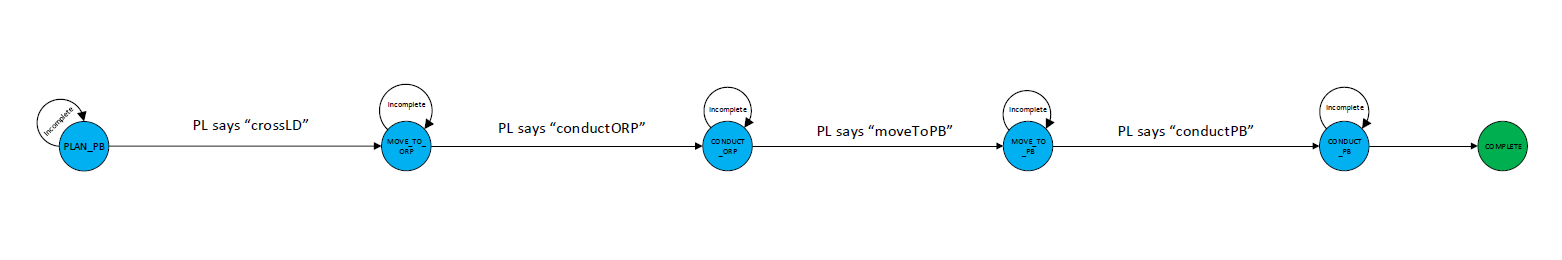
\includegraphics[width=1\linewidth]{map32.png}
  \caption{PB Top Level States Overview}
\end{figure}
The states were organized into discrete subtasks, illustrated in figure 3.2
with blue circles and the state’s name in the center. Each state had easily
discernable actions for entering and exiting the state, given above the line
connecting adjacent states. For simplicity, the majority of commands were
just named after the state that would be initiated when the command was given
(i.e. moveToPB initiates the MOVE_TO_PB state), with the exceptions of the
PLAN_PB state which would be initiated by Higher Head Quarters (HHQ) when they
transmitted an operations order (OPORD) and the MOVE_TO_ORP state which would be
initiated by the command given by the Platoon Leader (PL) to cross the line of
departure (LD).\\\\
Each state was given a loop, labeled “incomplete,” which would simply
allow the Platoon time to execute the tasks associated with each state.\\\\
We recognized that the state machine we initially designed, here after
referred to as top-level state machine, required alternate states that
would represent conclusions other than a successful completion of a PB.
Three scenarios were derived:
\begin{enumerate}
\item The Platoon received a new mission.
\item The Platoon came under attack.
\item The Platoon was rendered non-mission capable (NMC) by either
  casualty (i.e. too many Soldiers fell ill or died), or lack of supplies.
\end{enumerate}
States corresponding to these scenarios were developed: “change mission,”
“react to contact,” and “return to base” respectively (illustrated in figure
3.3 with red circles). At any state in the PB top-level state machine, save
for the “complete” state which represents a successful PB operation, these
alternate termination states could be reached and essentially terminate the
machines execution (see figure 3.3).\\
\begin{figure}[h]
  \centering
  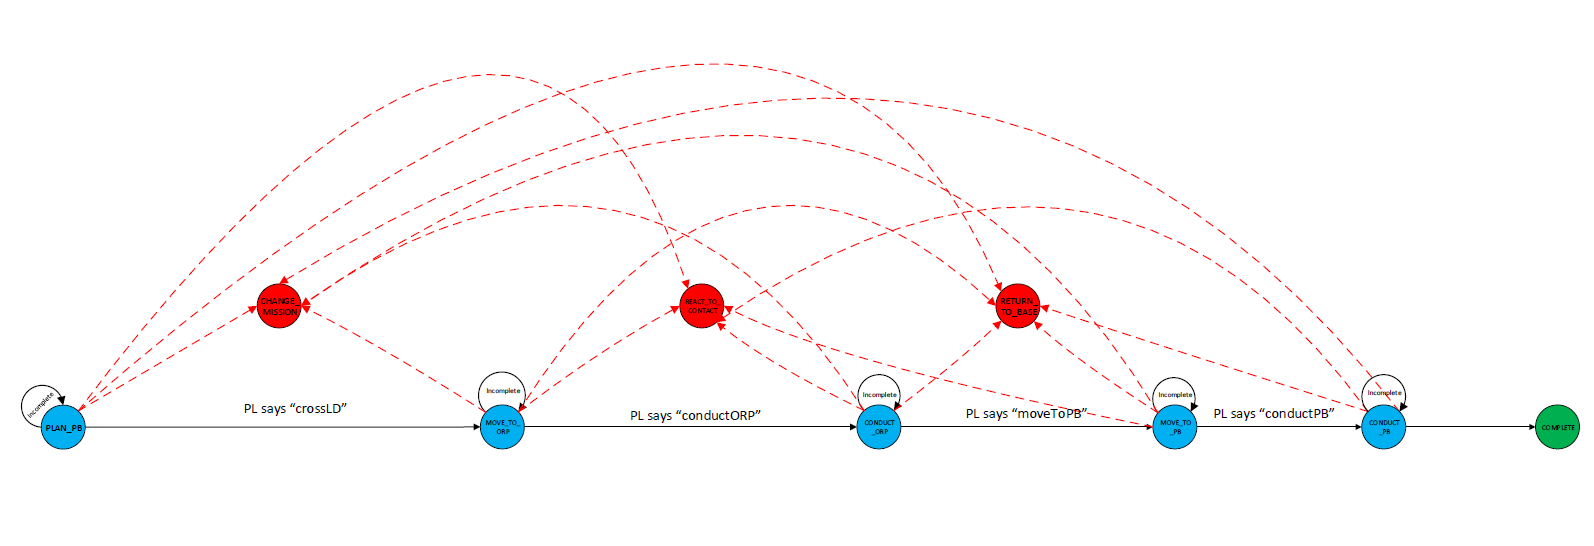
\includegraphics[width=1\linewidth]{map33.png}
  \caption{PB Top Level Alternate States Overview}
\end{figure}\\
Each of the top-level states represented a number of explicit tasks that
we extrapolated from the Ranger Handbook (Ranger Handbook 2011):
\begin{itemize}
\item The planning state for the PB (PLAN_PB) contained sub states
  corresponding to the “Troop Leading Procedures” (TLPs) outlined in
  chapter 2 section 1 of the Ranger Handbook (Ranger Handbook 2011, 23).
\item Movement to the objective rally point (MOVE_TO_ORP) sub
  states were crafted from chapter 6 (Ranger Handbook 2011, 101).
\item Sub states corresponding to the were found in chapter 7,
  section 20 (Ranger Handbook 2011, 131).
\item “Move to PB” sub states were formed similarly to those in “move to ORP.”
\item “Conduct PB” sub states were outlined by chapter 7 as well, section 21
  (Ranger Handbook 2011, 132).
\end{itemize}
From this we were able to develop sub states for each of the top-level
states (see figure 3.4).\\
\begin{figure}[h]
  \centering
  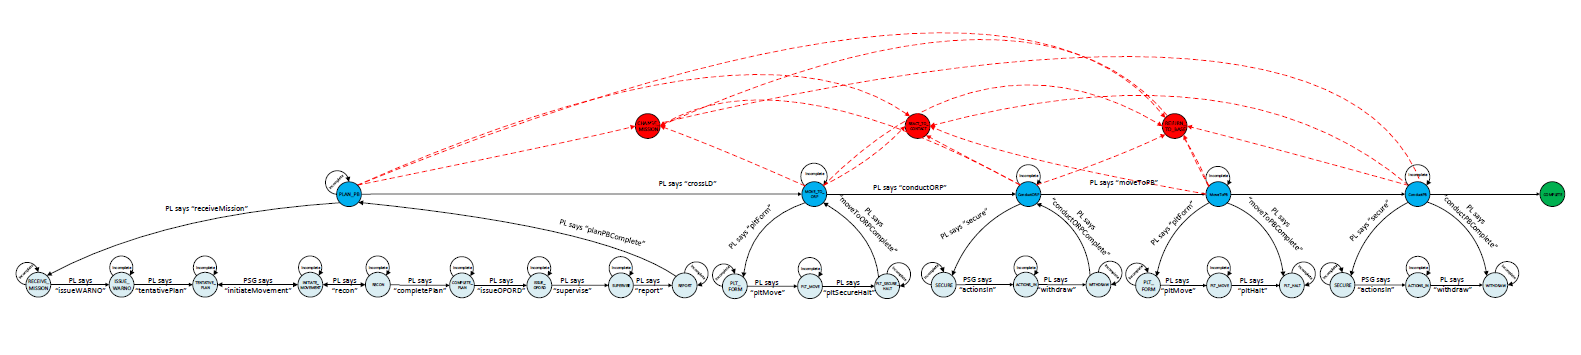
\includegraphics[width=1\linewidth]{map34.png}
  \caption{PB Sub States Overview}
\end{figure}\\
These sub states (shown in light blue in figure 3.4) not only provided a
finer granularity to the tasks within the PB, but also introduced new leadership
roles. The top-level state machine was controlled by only the PL, the sub state
machine had states that were initiated by the PL and the Platoon Sergeant (PSG)
(see figure 3.4).\\ \\
The sub states within the top-level state PLAN_PB presented another interesting
characteristic: according to the Ranger Handbook section 2-1 many of the states
could be executed in any order (Ranger Handbook 2011, 23). Specifically, out of
the eight steps to the TLP, the last five (see figure 3.5) (Ranger Handbook 2011,
23).\\
\begin{figure}[h]
  \centering
  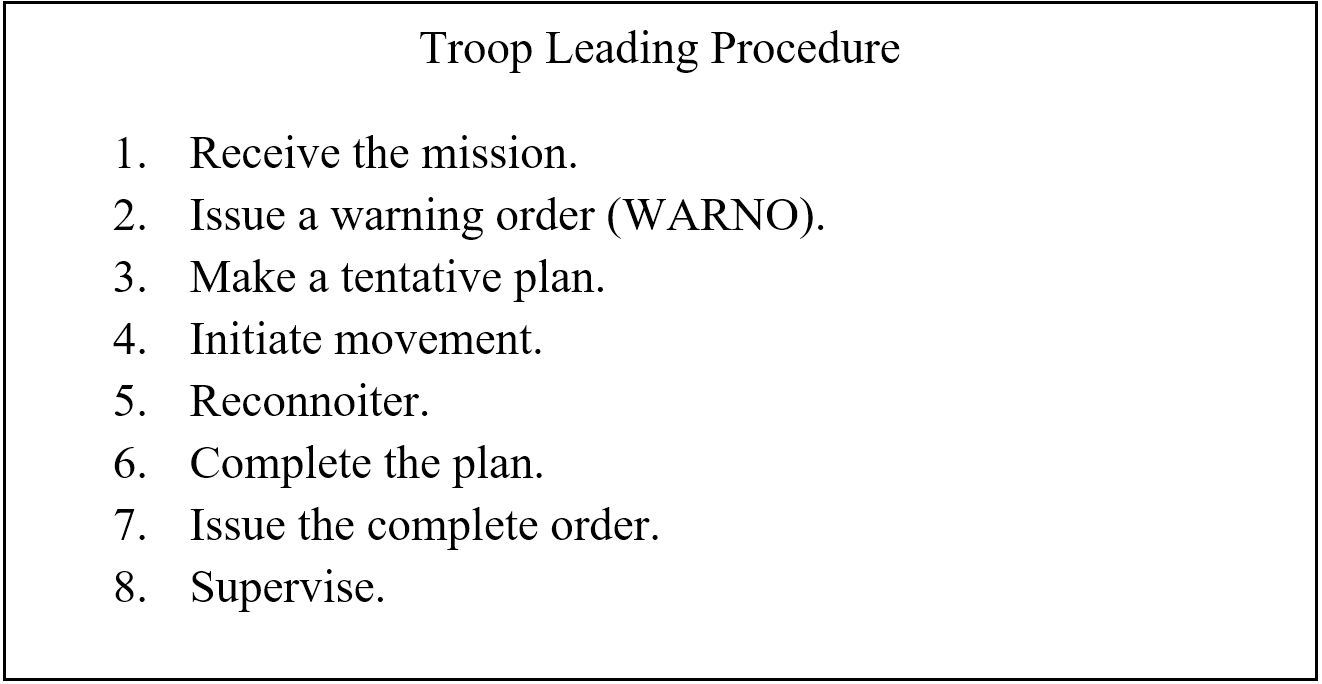
\includegraphics[width=0.6\linewidth]{map35.PNG}
  \caption{TLP Steps}
\end{figure}\\
We decided on a more logical, and smaller scale, approach. Issuing a complete order,
step 6, would require that the PL had already done the recon and used terrain analysis
to provide a complete plan. In the same regard, issuing a complete order, step 7,
requires that you have completed step 6. Consequently, there were only three states
within the top-level state PLAN_PB that would be allowed to initiate and terminate
out of order: TENTATIVE_PLAN, INITIATE_MOVEMENT, and RECON corresponding to the TLP
steps 3-5. These steps are outlined in orange in figure 3.6 below.\\
\begin{figure}[h]
  \centering
  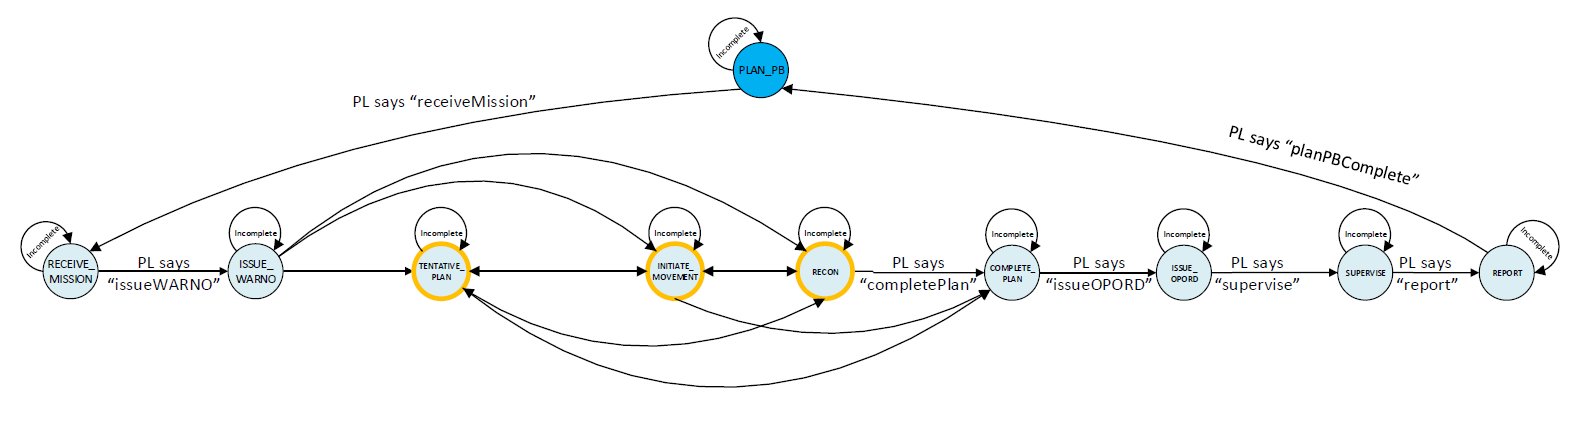
\includegraphics[width=1\linewidth]{map36.png}
  \caption{TLP PLAN_PB unordered sub states}
\end{figure}\\ \\

% ---- this points LaTeX to PatrolBaseDoc.tex ----
% Local Variables:
% TeX-master: "../PatrolBaseDoc"
% End:

%%made changes

\chapter{Results and Discussions}
\label{cha:results-discussions}
\newcommand{\HOLPBTypeDate}{09 July 2017}
\newcommand{\HOLPBTypeTime}{22:25}
\begin{SaveVerbatim}{HOLPBTypeDatatypesslCommand}
\HOLFreeVar{slCommand} = \HOLConst{crossLD} \HOLTokenBar{} \HOLConst{conductORP} \HOLTokenBar{} \HOLConst{moveToPB} \HOLTokenBar{} \HOLConst{conductPB}
          \HOLTokenBar{} \HOLConst{completePB} \HOLTokenBar{} \HOLConst{incomplete}
\end{SaveVerbatim}
\newcommand{\HOLPBTypeDatatypesslCommand}{\UseVerbatim{HOLPBTypeDatatypesslCommand}}
\begin{SaveVerbatim}{HOLPBTypeDatatypesslOutput}
\HOLFreeVar{slOutput} = \HOLConst{PlanPB} \HOLTokenBar{} \HOLConst{MoveToORP} \HOLTokenBar{} \HOLConst{ConductORP} \HOLTokenBar{} \HOLConst{MoveToPB}
         \HOLTokenBar{} \HOLConst{ConductPB} \HOLTokenBar{} \HOLConst{CompletePB} \HOLTokenBar{} \HOLConst{unAuthenticated}
\end{SaveVerbatim}
\newcommand{\HOLPBTypeDatatypesslOutput}{\UseVerbatim{HOLPBTypeDatatypesslOutput}}
\begin{SaveVerbatim}{HOLPBTypeDatatypesslState}
\HOLFreeVar{slState} = \HOLConst{PLAN_PB} \HOLTokenBar{} \HOLConst{MOVE_TO_ORP} \HOLTokenBar{} \HOLConst{CONDUCT_ORP} \HOLTokenBar{} \HOLConst{MOVE_TO_PB}
        \HOLTokenBar{} \HOLConst{CONDUCT_PB} \HOLTokenBar{} \HOLConst{COMPLETE_PB}
\end{SaveVerbatim}
\newcommand{\HOLPBTypeDatatypesslState}{\UseVerbatim{HOLPBTypeDatatypesslState}}
\begin{SaveVerbatim}{HOLPBTypeDatatypesstateRole}
\HOLFreeVar{stateRole} = \HOLConst{PlatoonLeader}
\end{SaveVerbatim}
\newcommand{\HOLPBTypeDatatypesstateRole}{\UseVerbatim{HOLPBTypeDatatypesstateRole}}
\newcommand{\HOLPBTypeDatatypes}{
\HOLPBTypeDatatypesslCommand\HOLPBTypeDatatypesslOutput\HOLPBTypeDatatypesslState\HOLPBTypeDatatypesstateRole}
\begin{SaveVerbatim}{HOLPBTypeTheoremsslCommandXXdistinctXXclauses}
\HOLTokenTurnstile{} \HOLConst{crossLD} \HOLSymConst{\HOLTokenNotEqual{}} \HOLConst{conductORP} \HOLSymConst{\HOLTokenConj{}} \HOLConst{crossLD} \HOLSymConst{\HOLTokenNotEqual{}} \HOLConst{moveToPB} \HOLSymConst{\HOLTokenConj{}}
   \HOLConst{crossLD} \HOLSymConst{\HOLTokenNotEqual{}} \HOLConst{conductPB} \HOLSymConst{\HOLTokenConj{}} \HOLConst{crossLD} \HOLSymConst{\HOLTokenNotEqual{}} \HOLConst{completePB} \HOLSymConst{\HOLTokenConj{}}
   \HOLConst{crossLD} \HOLSymConst{\HOLTokenNotEqual{}} \HOLConst{incomplete} \HOLSymConst{\HOLTokenConj{}} \HOLConst{conductORP} \HOLSymConst{\HOLTokenNotEqual{}} \HOLConst{moveToPB} \HOLSymConst{\HOLTokenConj{}}
   \HOLConst{conductORP} \HOLSymConst{\HOLTokenNotEqual{}} \HOLConst{conductPB} \HOLSymConst{\HOLTokenConj{}} \HOLConst{conductORP} \HOLSymConst{\HOLTokenNotEqual{}} \HOLConst{completePB} \HOLSymConst{\HOLTokenConj{}}
   \HOLConst{conductORP} \HOLSymConst{\HOLTokenNotEqual{}} \HOLConst{incomplete} \HOLSymConst{\HOLTokenConj{}} \HOLConst{moveToPB} \HOLSymConst{\HOLTokenNotEqual{}} \HOLConst{conductPB} \HOLSymConst{\HOLTokenConj{}}
   \HOLConst{moveToPB} \HOLSymConst{\HOLTokenNotEqual{}} \HOLConst{completePB} \HOLSymConst{\HOLTokenConj{}} \HOLConst{moveToPB} \HOLSymConst{\HOLTokenNotEqual{}} \HOLConst{incomplete} \HOLSymConst{\HOLTokenConj{}}
   \HOLConst{conductPB} \HOLSymConst{\HOLTokenNotEqual{}} \HOLConst{completePB} \HOLSymConst{\HOLTokenConj{}} \HOLConst{conductPB} \HOLSymConst{\HOLTokenNotEqual{}} \HOLConst{incomplete} \HOLSymConst{\HOLTokenConj{}}
   \HOLConst{completePB} \HOLSymConst{\HOLTokenNotEqual{}} \HOLConst{incomplete}
\end{SaveVerbatim}
\newcommand{\HOLPBTypeTheoremsslCommandXXdistinctXXclauses}{\UseVerbatim{HOLPBTypeTheoremsslCommandXXdistinctXXclauses}}
\begin{SaveVerbatim}{HOLPBTypeTheoremsslOutputXXdistinctXXclauses}
\HOLTokenTurnstile{} \HOLConst{PlanPB} \HOLSymConst{\HOLTokenNotEqual{}} \HOLConst{MoveToORP} \HOLSymConst{\HOLTokenConj{}} \HOLConst{PlanPB} \HOLSymConst{\HOLTokenNotEqual{}} \HOLConst{ConductORP} \HOLSymConst{\HOLTokenConj{}}
   \HOLConst{PlanPB} \HOLSymConst{\HOLTokenNotEqual{}} \HOLConst{MoveToPB} \HOLSymConst{\HOLTokenConj{}} \HOLConst{PlanPB} \HOLSymConst{\HOLTokenNotEqual{}} \HOLConst{ConductPB} \HOLSymConst{\HOLTokenConj{}}
   \HOLConst{PlanPB} \HOLSymConst{\HOLTokenNotEqual{}} \HOLConst{CompletePB} \HOLSymConst{\HOLTokenConj{}} \HOLConst{PlanPB} \HOLSymConst{\HOLTokenNotEqual{}} \HOLConst{unAuthenticated} \HOLSymConst{\HOLTokenConj{}}
   \HOLConst{MoveToORP} \HOLSymConst{\HOLTokenNotEqual{}} \HOLConst{ConductORP} \HOLSymConst{\HOLTokenConj{}} \HOLConst{MoveToORP} \HOLSymConst{\HOLTokenNotEqual{}} \HOLConst{MoveToPB} \HOLSymConst{\HOLTokenConj{}}
   \HOLConst{MoveToORP} \HOLSymConst{\HOLTokenNotEqual{}} \HOLConst{ConductPB} \HOLSymConst{\HOLTokenConj{}} \HOLConst{MoveToORP} \HOLSymConst{\HOLTokenNotEqual{}} \HOLConst{CompletePB} \HOLSymConst{\HOLTokenConj{}}
   \HOLConst{MoveToORP} \HOLSymConst{\HOLTokenNotEqual{}} \HOLConst{unAuthenticated} \HOLSymConst{\HOLTokenConj{}} \HOLConst{ConductORP} \HOLSymConst{\HOLTokenNotEqual{}} \HOLConst{MoveToPB} \HOLSymConst{\HOLTokenConj{}}
   \HOLConst{ConductORP} \HOLSymConst{\HOLTokenNotEqual{}} \HOLConst{ConductPB} \HOLSymConst{\HOLTokenConj{}} \HOLConst{ConductORP} \HOLSymConst{\HOLTokenNotEqual{}} \HOLConst{CompletePB} \HOLSymConst{\HOLTokenConj{}}
   \HOLConst{ConductORP} \HOLSymConst{\HOLTokenNotEqual{}} \HOLConst{unAuthenticated} \HOLSymConst{\HOLTokenConj{}} \HOLConst{MoveToPB} \HOLSymConst{\HOLTokenNotEqual{}} \HOLConst{ConductPB} \HOLSymConst{\HOLTokenConj{}}
   \HOLConst{MoveToPB} \HOLSymConst{\HOLTokenNotEqual{}} \HOLConst{CompletePB} \HOLSymConst{\HOLTokenConj{}} \HOLConst{MoveToPB} \HOLSymConst{\HOLTokenNotEqual{}} \HOLConst{unAuthenticated} \HOLSymConst{\HOLTokenConj{}}
   \HOLConst{ConductPB} \HOLSymConst{\HOLTokenNotEqual{}} \HOLConst{CompletePB} \HOLSymConst{\HOLTokenConj{}} \HOLConst{ConductPB} \HOLSymConst{\HOLTokenNotEqual{}} \HOLConst{unAuthenticated} \HOLSymConst{\HOLTokenConj{}}
   \HOLConst{CompletePB} \HOLSymConst{\HOLTokenNotEqual{}} \HOLConst{unAuthenticated}
\end{SaveVerbatim}
\newcommand{\HOLPBTypeTheoremsslOutputXXdistinctXXclauses}{\UseVerbatim{HOLPBTypeTheoremsslOutputXXdistinctXXclauses}}
\begin{SaveVerbatim}{HOLPBTypeTheoremsslStateXXdistinctXXclauses}
\HOLTokenTurnstile{} \HOLConst{PLAN_PB} \HOLSymConst{\HOLTokenNotEqual{}} \HOLConst{MOVE_TO_ORP} \HOLSymConst{\HOLTokenConj{}} \HOLConst{PLAN_PB} \HOLSymConst{\HOLTokenNotEqual{}} \HOLConst{CONDUCT_ORP} \HOLSymConst{\HOLTokenConj{}}
   \HOLConst{PLAN_PB} \HOLSymConst{\HOLTokenNotEqual{}} \HOLConst{MOVE_TO_PB} \HOLSymConst{\HOLTokenConj{}} \HOLConst{PLAN_PB} \HOLSymConst{\HOLTokenNotEqual{}} \HOLConst{CONDUCT_PB} \HOLSymConst{\HOLTokenConj{}}
   \HOLConst{PLAN_PB} \HOLSymConst{\HOLTokenNotEqual{}} \HOLConst{COMPLETE_PB} \HOLSymConst{\HOLTokenConj{}} \HOLConst{MOVE_TO_ORP} \HOLSymConst{\HOLTokenNotEqual{}} \HOLConst{CONDUCT_ORP} \HOLSymConst{\HOLTokenConj{}}
   \HOLConst{MOVE_TO_ORP} \HOLSymConst{\HOLTokenNotEqual{}} \HOLConst{MOVE_TO_PB} \HOLSymConst{\HOLTokenConj{}} \HOLConst{MOVE_TO_ORP} \HOLSymConst{\HOLTokenNotEqual{}} \HOLConst{CONDUCT_PB} \HOLSymConst{\HOLTokenConj{}}
   \HOLConst{MOVE_TO_ORP} \HOLSymConst{\HOLTokenNotEqual{}} \HOLConst{COMPLETE_PB} \HOLSymConst{\HOLTokenConj{}} \HOLConst{CONDUCT_ORP} \HOLSymConst{\HOLTokenNotEqual{}} \HOLConst{MOVE_TO_PB} \HOLSymConst{\HOLTokenConj{}}
   \HOLConst{CONDUCT_ORP} \HOLSymConst{\HOLTokenNotEqual{}} \HOLConst{CONDUCT_PB} \HOLSymConst{\HOLTokenConj{}} \HOLConst{CONDUCT_ORP} \HOLSymConst{\HOLTokenNotEqual{}} \HOLConst{COMPLETE_PB} \HOLSymConst{\HOLTokenConj{}}
   \HOLConst{MOVE_TO_PB} \HOLSymConst{\HOLTokenNotEqual{}} \HOLConst{CONDUCT_PB} \HOLSymConst{\HOLTokenConj{}} \HOLConst{MOVE_TO_PB} \HOLSymConst{\HOLTokenNotEqual{}} \HOLConst{COMPLETE_PB} \HOLSymConst{\HOLTokenConj{}}
   \HOLConst{CONDUCT_PB} \HOLSymConst{\HOLTokenNotEqual{}} \HOLConst{COMPLETE_PB}
\end{SaveVerbatim}
\newcommand{\HOLPBTypeTheoremsslStateXXdistinctXXclauses}{\UseVerbatim{HOLPBTypeTheoremsslStateXXdistinctXXclauses}}
\newcommand{\HOLPBTypeTheorems}{
\HOLThmTag{PBType}{slCommand_distinct_clauses}\HOLPBTypeTheoremsslCommandXXdistinctXXclauses
\HOLThmTag{PBType}{slOutput_distinct_clauses}\HOLPBTypeTheoremsslOutputXXdistinctXXclauses
\HOLThmTag{PBType}{slState_distinct_clauses}\HOLPBTypeTheoremsslStateXXdistinctXXclauses
}

\newcommand{\HOLssmPBDate}{02 July 2017}
\newcommand{\HOLssmPBTime}{22:51}
\begin{SaveVerbatim}{HOLssmPBDefinitionssecContextXXdef}
\HOLTokenTurnstile{} \HOLSymConst{\HOLTokenForall{}}\HOLBoundVar{slCommand}.
     \HOLConst{secContext} \HOLBoundVar{slCommand} \HOLSymConst{=}
     [\HOLConst{Name} \HOLConst{PlatoonLeader} \HOLConst{controls} \HOLConst{prop} (\HOLConst{SOME} (\HOLConst{SLc} \HOLBoundVar{slCommand}))]
\end{SaveVerbatim}
\newcommand{\HOLssmPBDefinitionssecContextXXdef}{\UseVerbatim{HOLssmPBDefinitionssecContextXXdef}}
\begin{SaveVerbatim}{HOLssmPBDefinitionsssmPBStateInterpXXdef}
\HOLTokenTurnstile{} \HOLSymConst{\HOLTokenForall{}}\HOLBoundVar{state}. \HOLConst{ssmPBStateInterp} \HOLBoundVar{state} \HOLSymConst{=} \HOLConst{TT}
\end{SaveVerbatim}
\newcommand{\HOLssmPBDefinitionsssmPBStateInterpXXdef}{\UseVerbatim{HOLssmPBDefinitionsssmPBStateInterpXXdef}}
\newcommand{\HOLssmPBDefinitions}{
\HOLDfnTag{ssmPB}{secContext_def}\HOLssmPBDefinitionssecContextXXdef
\HOLDfnTag{ssmPB}{ssmPBStateInterp_def}\HOLssmPBDefinitionsssmPBStateInterpXXdef
}
\begin{SaveVerbatim}{HOLssmPBTheoremsauthenticationTestXXcmdXXrejectXXlemma}
\HOLTokenTurnstile{} \HOLSymConst{\HOLTokenForall{}}\HOLBoundVar{cmd}. \HOLSymConst{\HOLTokenNeg{}}\HOLConst{authenticationTest} (\HOLConst{prop} (\HOLConst{SOME} \HOLBoundVar{cmd}))
\end{SaveVerbatim}
\newcommand{\HOLssmPBTheoremsauthenticationTestXXcmdXXrejectXXlemma}{\UseVerbatim{HOLssmPBTheoremsauthenticationTestXXcmdXXrejectXXlemma}}
\begin{SaveVerbatim}{HOLssmPBTheoremsauthenticationTestXXdef}
\HOLTokenTurnstile{} (\HOLConst{authenticationTest} (\HOLConst{Name} \HOLConst{PlatoonLeader} \HOLConst{says} \HOLConst{prop} \HOLFreeVar{cmd}) \HOLSymConst{\HOLTokenEquiv{}}
    \HOLConst{T}) \HOLSymConst{\HOLTokenConj{}} (\HOLConst{authenticationTest} \HOLConst{TT} \HOLSymConst{\HOLTokenEquiv{}} \HOLConst{F}) \HOLSymConst{\HOLTokenConj{}}
   (\HOLConst{authenticationTest} \HOLConst{FF} \HOLSymConst{\HOLTokenEquiv{}} \HOLConst{F}) \HOLSymConst{\HOLTokenConj{}}
   (\HOLConst{authenticationTest} (\HOLConst{prop} \HOLFreeVar{v}) \HOLSymConst{\HOLTokenEquiv{}} \HOLConst{F}) \HOLSymConst{\HOLTokenConj{}}
   (\HOLConst{authenticationTest} (\HOLConst{notf} \HOLFreeVar{v\sb{\mathrm{1}}}) \HOLSymConst{\HOLTokenEquiv{}} \HOLConst{F}) \HOLSymConst{\HOLTokenConj{}}
   (\HOLConst{authenticationTest} (\HOLFreeVar{v\sb{\mathrm{2}}} \HOLConst{andf} \HOLFreeVar{v\sb{\mathrm{3}}}) \HOLSymConst{\HOLTokenEquiv{}} \HOLConst{F}) \HOLSymConst{\HOLTokenConj{}}
   (\HOLConst{authenticationTest} (\HOLFreeVar{v\sb{\mathrm{4}}} \HOLConst{orf} \HOLFreeVar{v\sb{\mathrm{5}}}) \HOLSymConst{\HOLTokenEquiv{}} \HOLConst{F}) \HOLSymConst{\HOLTokenConj{}}
   (\HOLConst{authenticationTest} (\HOLFreeVar{v\sb{\mathrm{6}}} \HOLConst{impf} \HOLFreeVar{v\sb{\mathrm{7}}}) \HOLSymConst{\HOLTokenEquiv{}} \HOLConst{F}) \HOLSymConst{\HOLTokenConj{}}
   (\HOLConst{authenticationTest} (\HOLFreeVar{v\sb{\mathrm{8}}} \HOLConst{eqf} \HOLFreeVar{v\sb{\mathrm{9}}}) \HOLSymConst{\HOLTokenEquiv{}} \HOLConst{F}) \HOLSymConst{\HOLTokenConj{}}
   (\HOLConst{authenticationTest} (\HOLFreeVar{v\sb{\mathrm{10}}} \HOLConst{says} \HOLConst{TT}) \HOLSymConst{\HOLTokenEquiv{}} \HOLConst{F}) \HOLSymConst{\HOLTokenConj{}}
   (\HOLConst{authenticationTest} (\HOLFreeVar{v\sb{\mathrm{10}}} \HOLConst{says} \HOLConst{FF}) \HOLSymConst{\HOLTokenEquiv{}} \HOLConst{F}) \HOLSymConst{\HOLTokenConj{}}
   (\HOLConst{authenticationTest} (\HOLFreeVar{v133} \HOLConst{meet} \HOLFreeVar{v134} \HOLConst{says} \HOLConst{prop} \HOLFreeVar{v\sb{\mathrm{66}}}) \HOLSymConst{\HOLTokenEquiv{}} \HOLConst{F}) \HOLSymConst{\HOLTokenConj{}}
   (\HOLConst{authenticationTest} (\HOLFreeVar{v135} \HOLConst{quoting} \HOLFreeVar{v136} \HOLConst{says} \HOLConst{prop} \HOLFreeVar{v\sb{\mathrm{66}}}) \HOLSymConst{\HOLTokenEquiv{}} \HOLConst{F}) \HOLSymConst{\HOLTokenConj{}}
   (\HOLConst{authenticationTest} (\HOLFreeVar{v\sb{\mathrm{10}}} \HOLConst{says} \HOLConst{notf} \HOLFreeVar{v\sb{\mathrm{67}}}) \HOLSymConst{\HOLTokenEquiv{}} \HOLConst{F}) \HOLSymConst{\HOLTokenConj{}}
   (\HOLConst{authenticationTest} (\HOLFreeVar{v\sb{\mathrm{10}}} \HOLConst{says} (\HOLFreeVar{v\sb{\mathrm{68}}} \HOLConst{andf} \HOLFreeVar{v\sb{\mathrm{69}}})) \HOLSymConst{\HOLTokenEquiv{}} \HOLConst{F}) \HOLSymConst{\HOLTokenConj{}}
   (\HOLConst{authenticationTest} (\HOLFreeVar{v\sb{\mathrm{10}}} \HOLConst{says} (\HOLFreeVar{v\sb{\mathrm{70}}} \HOLConst{orf} \HOLFreeVar{v\sb{\mathrm{71}}})) \HOLSymConst{\HOLTokenEquiv{}} \HOLConst{F}) \HOLSymConst{\HOLTokenConj{}}
   (\HOLConst{authenticationTest} (\HOLFreeVar{v\sb{\mathrm{10}}} \HOLConst{says} (\HOLFreeVar{v\sb{\mathrm{72}}} \HOLConst{impf} \HOLFreeVar{v\sb{\mathrm{73}}})) \HOLSymConst{\HOLTokenEquiv{}} \HOLConst{F}) \HOLSymConst{\HOLTokenConj{}}
   (\HOLConst{authenticationTest} (\HOLFreeVar{v\sb{\mathrm{10}}} \HOLConst{says} (\HOLFreeVar{v\sb{\mathrm{74}}} \HOLConst{eqf} \HOLFreeVar{v\sb{\mathrm{75}}})) \HOLSymConst{\HOLTokenEquiv{}} \HOLConst{F}) \HOLSymConst{\HOLTokenConj{}}
   (\HOLConst{authenticationTest} (\HOLFreeVar{v\sb{\mathrm{10}}} \HOLConst{says} \HOLFreeVar{v\sb{\mathrm{76}}} \HOLConst{says} \HOLFreeVar{v\sb{\mathrm{77}}}) \HOLSymConst{\HOLTokenEquiv{}} \HOLConst{F}) \HOLSymConst{\HOLTokenConj{}}
   (\HOLConst{authenticationTest} (\HOLFreeVar{v\sb{\mathrm{10}}} \HOLConst{says} \HOLFreeVar{v\sb{\mathrm{78}}} \HOLConst{speaks_for} \HOLFreeVar{v\sb{\mathrm{79}}}) \HOLSymConst{\HOLTokenEquiv{}} \HOLConst{F}) \HOLSymConst{\HOLTokenConj{}}
   (\HOLConst{authenticationTest} (\HOLFreeVar{v\sb{\mathrm{10}}} \HOLConst{says} \HOLFreeVar{v\sb{\mathrm{80}}} \HOLConst{controls} \HOLFreeVar{v\sb{\mathrm{81}}}) \HOLSymConst{\HOLTokenEquiv{}} \HOLConst{F}) \HOLSymConst{\HOLTokenConj{}}
   (\HOLConst{authenticationTest} (\HOLFreeVar{v\sb{\mathrm{10}}} \HOLConst{says} \HOLConst{reps} \HOLFreeVar{v\sb{\mathrm{82}}} \HOLFreeVar{v\sb{\mathrm{83}}} \HOLFreeVar{v\sb{\mathrm{84}}}) \HOLSymConst{\HOLTokenEquiv{}} \HOLConst{F}) \HOLSymConst{\HOLTokenConj{}}
   (\HOLConst{authenticationTest} (\HOLFreeVar{v\sb{\mathrm{10}}} \HOLConst{says} \HOLFreeVar{v\sb{\mathrm{85}}} \HOLConst{domi} \HOLFreeVar{v\sb{\mathrm{86}}}) \HOLSymConst{\HOLTokenEquiv{}} \HOLConst{F}) \HOLSymConst{\HOLTokenConj{}}
   (\HOLConst{authenticationTest} (\HOLFreeVar{v\sb{\mathrm{10}}} \HOLConst{says} \HOLFreeVar{v\sb{\mathrm{87}}} \HOLConst{eqi} \HOLFreeVar{v\sb{\mathrm{88}}}) \HOLSymConst{\HOLTokenEquiv{}} \HOLConst{F}) \HOLSymConst{\HOLTokenConj{}}
   (\HOLConst{authenticationTest} (\HOLFreeVar{v\sb{\mathrm{10}}} \HOLConst{says} \HOLFreeVar{v\sb{\mathrm{89}}} \HOLConst{doms} \HOLFreeVar{v\sb{\mathrm{90}}}) \HOLSymConst{\HOLTokenEquiv{}} \HOLConst{F}) \HOLSymConst{\HOLTokenConj{}}
   (\HOLConst{authenticationTest} (\HOLFreeVar{v\sb{\mathrm{10}}} \HOLConst{says} \HOLFreeVar{v\sb{\mathrm{91}}} \HOLConst{eqs} \HOLFreeVar{v\sb{\mathrm{92}}}) \HOLSymConst{\HOLTokenEquiv{}} \HOLConst{F}) \HOLSymConst{\HOLTokenConj{}}
   (\HOLConst{authenticationTest} (\HOLFreeVar{v\sb{\mathrm{10}}} \HOLConst{says} \HOLFreeVar{v\sb{\mathrm{93}}} \HOLConst{eqn} \HOLFreeVar{v\sb{\mathrm{94}}}) \HOLSymConst{\HOLTokenEquiv{}} \HOLConst{F}) \HOLSymConst{\HOLTokenConj{}}
   (\HOLConst{authenticationTest} (\HOLFreeVar{v\sb{\mathrm{10}}} \HOLConst{says} \HOLFreeVar{v\sb{\mathrm{95}}} \HOLConst{lte} \HOLFreeVar{v\sb{\mathrm{96}}}) \HOLSymConst{\HOLTokenEquiv{}} \HOLConst{F}) \HOLSymConst{\HOLTokenConj{}}
   (\HOLConst{authenticationTest} (\HOLFreeVar{v\sb{\mathrm{10}}} \HOLConst{says} \HOLFreeVar{v\sb{\mathrm{97}}} \HOLConst{lt} \HOLFreeVar{v\sb{\mathrm{98}}}) \HOLSymConst{\HOLTokenEquiv{}} \HOLConst{F}) \HOLSymConst{\HOLTokenConj{}}
   (\HOLConst{authenticationTest} (\HOLFreeVar{v\sb{\mathrm{12}}} \HOLConst{speaks_for} \HOLFreeVar{v\sb{\mathrm{13}}}) \HOLSymConst{\HOLTokenEquiv{}} \HOLConst{F}) \HOLSymConst{\HOLTokenConj{}}
   (\HOLConst{authenticationTest} (\HOLFreeVar{v\sb{\mathrm{14}}} \HOLConst{controls} \HOLFreeVar{v\sb{\mathrm{15}}}) \HOLSymConst{\HOLTokenEquiv{}} \HOLConst{F}) \HOLSymConst{\HOLTokenConj{}}
   (\HOLConst{authenticationTest} (\HOLConst{reps} \HOLFreeVar{v\sb{\mathrm{16}}} \HOLFreeVar{v\sb{\mathrm{17}}} \HOLFreeVar{v\sb{\mathrm{18}}}) \HOLSymConst{\HOLTokenEquiv{}} \HOLConst{F}) \HOLSymConst{\HOLTokenConj{}}
   (\HOLConst{authenticationTest} (\HOLFreeVar{v\sb{\mathrm{19}}} \HOLConst{domi} \HOLFreeVar{v\sb{\mathrm{20}}}) \HOLSymConst{\HOLTokenEquiv{}} \HOLConst{F}) \HOLSymConst{\HOLTokenConj{}}
   (\HOLConst{authenticationTest} (\HOLFreeVar{v\sb{\mathrm{21}}} \HOLConst{eqi} \HOLFreeVar{v\sb{\mathrm{22}}}) \HOLSymConst{\HOLTokenEquiv{}} \HOLConst{F}) \HOLSymConst{\HOLTokenConj{}}
   (\HOLConst{authenticationTest} (\HOLFreeVar{v\sb{\mathrm{23}}} \HOLConst{doms} \HOLFreeVar{v\sb{\mathrm{24}}}) \HOLSymConst{\HOLTokenEquiv{}} \HOLConst{F}) \HOLSymConst{\HOLTokenConj{}}
   (\HOLConst{authenticationTest} (\HOLFreeVar{v\sb{\mathrm{25}}} \HOLConst{eqs} \HOLFreeVar{v\sb{\mathrm{26}}}) \HOLSymConst{\HOLTokenEquiv{}} \HOLConst{F}) \HOLSymConst{\HOLTokenConj{}}
   (\HOLConst{authenticationTest} (\HOLFreeVar{v\sb{\mathrm{27}}} \HOLConst{eqn} \HOLFreeVar{v\sb{\mathrm{28}}}) \HOLSymConst{\HOLTokenEquiv{}} \HOLConst{F}) \HOLSymConst{\HOLTokenConj{}}
   (\HOLConst{authenticationTest} (\HOLFreeVar{v\sb{\mathrm{29}}} \HOLConst{lte} \HOLFreeVar{v\sb{\mathrm{30}}}) \HOLSymConst{\HOLTokenEquiv{}} \HOLConst{F}) \HOLSymConst{\HOLTokenConj{}}
   (\HOLConst{authenticationTest} (\HOLFreeVar{v\sb{\mathrm{31}}} \HOLConst{lt} \HOLFreeVar{v\sb{\mathrm{32}}}) \HOLSymConst{\HOLTokenEquiv{}} \HOLConst{F})
\end{SaveVerbatim}
\newcommand{\HOLssmPBTheoremsauthenticationTestXXdef}{\UseVerbatim{HOLssmPBTheoremsauthenticationTestXXdef}}
\begin{SaveVerbatim}{HOLssmPBTheoremsauthenticationTestXXind}
\HOLTokenTurnstile{} \HOLSymConst{\HOLTokenForall{}}\HOLBoundVar{P}.
     (\HOLSymConst{\HOLTokenForall{}}\HOLBoundVar{cmd}. \HOLBoundVar{P} (\HOLConst{Name} \HOLConst{PlatoonLeader} \HOLConst{says} \HOLConst{prop} \HOLBoundVar{cmd})) \HOLSymConst{\HOLTokenConj{}} \HOLBoundVar{P} \HOLConst{TT} \HOLSymConst{\HOLTokenConj{}}
     \HOLBoundVar{P} \HOLConst{FF} \HOLSymConst{\HOLTokenConj{}} (\HOLSymConst{\HOLTokenForall{}}\HOLBoundVar{v}. \HOLBoundVar{P} (\HOLConst{prop} \HOLBoundVar{v})) \HOLSymConst{\HOLTokenConj{}} (\HOLSymConst{\HOLTokenForall{}}\HOLBoundVar{v\sb{\mathrm{1}}}. \HOLBoundVar{P} (\HOLConst{notf} \HOLBoundVar{v\sb{\mathrm{1}}})) \HOLSymConst{\HOLTokenConj{}}
     (\HOLSymConst{\HOLTokenForall{}}\HOLBoundVar{v\sb{\mathrm{2}}} \HOLBoundVar{v\sb{\mathrm{3}}}. \HOLBoundVar{P} (\HOLBoundVar{v\sb{\mathrm{2}}} \HOLConst{andf} \HOLBoundVar{v\sb{\mathrm{3}}})) \HOLSymConst{\HOLTokenConj{}} (\HOLSymConst{\HOLTokenForall{}}\HOLBoundVar{v\sb{\mathrm{4}}} \HOLBoundVar{v\sb{\mathrm{5}}}. \HOLBoundVar{P} (\HOLBoundVar{v\sb{\mathrm{4}}} \HOLConst{orf} \HOLBoundVar{v\sb{\mathrm{5}}})) \HOLSymConst{\HOLTokenConj{}}
     (\HOLSymConst{\HOLTokenForall{}}\HOLBoundVar{v\sb{\mathrm{6}}} \HOLBoundVar{v\sb{\mathrm{7}}}. \HOLBoundVar{P} (\HOLBoundVar{v\sb{\mathrm{6}}} \HOLConst{impf} \HOLBoundVar{v\sb{\mathrm{7}}})) \HOLSymConst{\HOLTokenConj{}} (\HOLSymConst{\HOLTokenForall{}}\HOLBoundVar{v\sb{\mathrm{8}}} \HOLBoundVar{v\sb{\mathrm{9}}}. \HOLBoundVar{P} (\HOLBoundVar{v\sb{\mathrm{8}}} \HOLConst{eqf} \HOLBoundVar{v\sb{\mathrm{9}}})) \HOLSymConst{\HOLTokenConj{}}
     (\HOLSymConst{\HOLTokenForall{}}\HOLBoundVar{v\sb{\mathrm{10}}}. \HOLBoundVar{P} (\HOLBoundVar{v\sb{\mathrm{10}}} \HOLConst{says} \HOLConst{TT})) \HOLSymConst{\HOLTokenConj{}} (\HOLSymConst{\HOLTokenForall{}}\HOLBoundVar{v\sb{\mathrm{10}}}. \HOLBoundVar{P} (\HOLBoundVar{v\sb{\mathrm{10}}} \HOLConst{says} \HOLConst{FF})) \HOLSymConst{\HOLTokenConj{}}
     (\HOLSymConst{\HOLTokenForall{}}\HOLBoundVar{v133} \HOLBoundVar{v134} \HOLBoundVar{v\sb{\mathrm{66}}}. \HOLBoundVar{P} (\HOLBoundVar{v133} \HOLConst{meet} \HOLBoundVar{v134} \HOLConst{says} \HOLConst{prop} \HOLBoundVar{v\sb{\mathrm{66}}})) \HOLSymConst{\HOLTokenConj{}}
     (\HOLSymConst{\HOLTokenForall{}}\HOLBoundVar{v135} \HOLBoundVar{v136} \HOLBoundVar{v\sb{\mathrm{66}}}. \HOLBoundVar{P} (\HOLBoundVar{v135} \HOLConst{quoting} \HOLBoundVar{v136} \HOLConst{says} \HOLConst{prop} \HOLBoundVar{v\sb{\mathrm{66}}})) \HOLSymConst{\HOLTokenConj{}}
     (\HOLSymConst{\HOLTokenForall{}}\HOLBoundVar{v\sb{\mathrm{10}}} \HOLBoundVar{v\sb{\mathrm{67}}}. \HOLBoundVar{P} (\HOLBoundVar{v\sb{\mathrm{10}}} \HOLConst{says} \HOLConst{notf} \HOLBoundVar{v\sb{\mathrm{67}}})) \HOLSymConst{\HOLTokenConj{}}
     (\HOLSymConst{\HOLTokenForall{}}\HOLBoundVar{v\sb{\mathrm{10}}} \HOLBoundVar{v\sb{\mathrm{68}}} \HOLBoundVar{v\sb{\mathrm{69}}}. \HOLBoundVar{P} (\HOLBoundVar{v\sb{\mathrm{10}}} \HOLConst{says} (\HOLBoundVar{v\sb{\mathrm{68}}} \HOLConst{andf} \HOLBoundVar{v\sb{\mathrm{69}}}))) \HOLSymConst{\HOLTokenConj{}}
     (\HOLSymConst{\HOLTokenForall{}}\HOLBoundVar{v\sb{\mathrm{10}}} \HOLBoundVar{v\sb{\mathrm{70}}} \HOLBoundVar{v\sb{\mathrm{71}}}. \HOLBoundVar{P} (\HOLBoundVar{v\sb{\mathrm{10}}} \HOLConst{says} (\HOLBoundVar{v\sb{\mathrm{70}}} \HOLConst{orf} \HOLBoundVar{v\sb{\mathrm{71}}}))) \HOLSymConst{\HOLTokenConj{}}
     (\HOLSymConst{\HOLTokenForall{}}\HOLBoundVar{v\sb{\mathrm{10}}} \HOLBoundVar{v\sb{\mathrm{72}}} \HOLBoundVar{v\sb{\mathrm{73}}}. \HOLBoundVar{P} (\HOLBoundVar{v\sb{\mathrm{10}}} \HOLConst{says} (\HOLBoundVar{v\sb{\mathrm{72}}} \HOLConst{impf} \HOLBoundVar{v\sb{\mathrm{73}}}))) \HOLSymConst{\HOLTokenConj{}}
     (\HOLSymConst{\HOLTokenForall{}}\HOLBoundVar{v\sb{\mathrm{10}}} \HOLBoundVar{v\sb{\mathrm{74}}} \HOLBoundVar{v\sb{\mathrm{75}}}. \HOLBoundVar{P} (\HOLBoundVar{v\sb{\mathrm{10}}} \HOLConst{says} (\HOLBoundVar{v\sb{\mathrm{74}}} \HOLConst{eqf} \HOLBoundVar{v\sb{\mathrm{75}}}))) \HOLSymConst{\HOLTokenConj{}}
     (\HOLSymConst{\HOLTokenForall{}}\HOLBoundVar{v\sb{\mathrm{10}}} \HOLBoundVar{v\sb{\mathrm{76}}} \HOLBoundVar{v\sb{\mathrm{77}}}. \HOLBoundVar{P} (\HOLBoundVar{v\sb{\mathrm{10}}} \HOLConst{says} \HOLBoundVar{v\sb{\mathrm{76}}} \HOLConst{says} \HOLBoundVar{v\sb{\mathrm{77}}})) \HOLSymConst{\HOLTokenConj{}}
     (\HOLSymConst{\HOLTokenForall{}}\HOLBoundVar{v\sb{\mathrm{10}}} \HOLBoundVar{v\sb{\mathrm{78}}} \HOLBoundVar{v\sb{\mathrm{79}}}. \HOLBoundVar{P} (\HOLBoundVar{v\sb{\mathrm{10}}} \HOLConst{says} \HOLBoundVar{v\sb{\mathrm{78}}} \HOLConst{speaks_for} \HOLBoundVar{v\sb{\mathrm{79}}})) \HOLSymConst{\HOLTokenConj{}}
     (\HOLSymConst{\HOLTokenForall{}}\HOLBoundVar{v\sb{\mathrm{10}}} \HOLBoundVar{v\sb{\mathrm{80}}} \HOLBoundVar{v\sb{\mathrm{81}}}. \HOLBoundVar{P} (\HOLBoundVar{v\sb{\mathrm{10}}} \HOLConst{says} \HOLBoundVar{v\sb{\mathrm{80}}} \HOLConst{controls} \HOLBoundVar{v\sb{\mathrm{81}}})) \HOLSymConst{\HOLTokenConj{}}
     (\HOLSymConst{\HOLTokenForall{}}\HOLBoundVar{v\sb{\mathrm{10}}} \HOLBoundVar{v\sb{\mathrm{82}}} \HOLBoundVar{v\sb{\mathrm{83}}} \HOLBoundVar{v\sb{\mathrm{84}}}. \HOLBoundVar{P} (\HOLBoundVar{v\sb{\mathrm{10}}} \HOLConst{says} \HOLConst{reps} \HOLBoundVar{v\sb{\mathrm{82}}} \HOLBoundVar{v\sb{\mathrm{83}}} \HOLBoundVar{v\sb{\mathrm{84}}})) \HOLSymConst{\HOLTokenConj{}}
     (\HOLSymConst{\HOLTokenForall{}}\HOLBoundVar{v\sb{\mathrm{10}}} \HOLBoundVar{v\sb{\mathrm{85}}} \HOLBoundVar{v\sb{\mathrm{86}}}. \HOLBoundVar{P} (\HOLBoundVar{v\sb{\mathrm{10}}} \HOLConst{says} \HOLBoundVar{v\sb{\mathrm{85}}} \HOLConst{domi} \HOLBoundVar{v\sb{\mathrm{86}}})) \HOLSymConst{\HOLTokenConj{}}
     (\HOLSymConst{\HOLTokenForall{}}\HOLBoundVar{v\sb{\mathrm{10}}} \HOLBoundVar{v\sb{\mathrm{87}}} \HOLBoundVar{v\sb{\mathrm{88}}}. \HOLBoundVar{P} (\HOLBoundVar{v\sb{\mathrm{10}}} \HOLConst{says} \HOLBoundVar{v\sb{\mathrm{87}}} \HOLConst{eqi} \HOLBoundVar{v\sb{\mathrm{88}}})) \HOLSymConst{\HOLTokenConj{}}
     (\HOLSymConst{\HOLTokenForall{}}\HOLBoundVar{v\sb{\mathrm{10}}} \HOLBoundVar{v\sb{\mathrm{89}}} \HOLBoundVar{v\sb{\mathrm{90}}}. \HOLBoundVar{P} (\HOLBoundVar{v\sb{\mathrm{10}}} \HOLConst{says} \HOLBoundVar{v\sb{\mathrm{89}}} \HOLConst{doms} \HOLBoundVar{v\sb{\mathrm{90}}})) \HOLSymConst{\HOLTokenConj{}}
     (\HOLSymConst{\HOLTokenForall{}}\HOLBoundVar{v\sb{\mathrm{10}}} \HOLBoundVar{v\sb{\mathrm{91}}} \HOLBoundVar{v\sb{\mathrm{92}}}. \HOLBoundVar{P} (\HOLBoundVar{v\sb{\mathrm{10}}} \HOLConst{says} \HOLBoundVar{v\sb{\mathrm{91}}} \HOLConst{eqs} \HOLBoundVar{v\sb{\mathrm{92}}})) \HOLSymConst{\HOLTokenConj{}}
     (\HOLSymConst{\HOLTokenForall{}}\HOLBoundVar{v\sb{\mathrm{10}}} \HOLBoundVar{v\sb{\mathrm{93}}} \HOLBoundVar{v\sb{\mathrm{94}}}. \HOLBoundVar{P} (\HOLBoundVar{v\sb{\mathrm{10}}} \HOLConst{says} \HOLBoundVar{v\sb{\mathrm{93}}} \HOLConst{eqn} \HOLBoundVar{v\sb{\mathrm{94}}})) \HOLSymConst{\HOLTokenConj{}}
     (\HOLSymConst{\HOLTokenForall{}}\HOLBoundVar{v\sb{\mathrm{10}}} \HOLBoundVar{v\sb{\mathrm{95}}} \HOLBoundVar{v\sb{\mathrm{96}}}. \HOLBoundVar{P} (\HOLBoundVar{v\sb{\mathrm{10}}} \HOLConst{says} \HOLBoundVar{v\sb{\mathrm{95}}} \HOLConst{lte} \HOLBoundVar{v\sb{\mathrm{96}}})) \HOLSymConst{\HOLTokenConj{}}
     (\HOLSymConst{\HOLTokenForall{}}\HOLBoundVar{v\sb{\mathrm{10}}} \HOLBoundVar{v\sb{\mathrm{97}}} \HOLBoundVar{v\sb{\mathrm{98}}}. \HOLBoundVar{P} (\HOLBoundVar{v\sb{\mathrm{10}}} \HOLConst{says} \HOLBoundVar{v\sb{\mathrm{97}}} \HOLConst{lt} \HOLBoundVar{v\sb{\mathrm{98}}})) \HOLSymConst{\HOLTokenConj{}}
     (\HOLSymConst{\HOLTokenForall{}}\HOLBoundVar{v\sb{\mathrm{12}}} \HOLBoundVar{v\sb{\mathrm{13}}}. \HOLBoundVar{P} (\HOLBoundVar{v\sb{\mathrm{12}}} \HOLConst{speaks_for} \HOLBoundVar{v\sb{\mathrm{13}}})) \HOLSymConst{\HOLTokenConj{}}
     (\HOLSymConst{\HOLTokenForall{}}\HOLBoundVar{v\sb{\mathrm{14}}} \HOLBoundVar{v\sb{\mathrm{15}}}. \HOLBoundVar{P} (\HOLBoundVar{v\sb{\mathrm{14}}} \HOLConst{controls} \HOLBoundVar{v\sb{\mathrm{15}}})) \HOLSymConst{\HOLTokenConj{}}
     (\HOLSymConst{\HOLTokenForall{}}\HOLBoundVar{v\sb{\mathrm{16}}} \HOLBoundVar{v\sb{\mathrm{17}}} \HOLBoundVar{v\sb{\mathrm{18}}}. \HOLBoundVar{P} (\HOLConst{reps} \HOLBoundVar{v\sb{\mathrm{16}}} \HOLBoundVar{v\sb{\mathrm{17}}} \HOLBoundVar{v\sb{\mathrm{18}}})) \HOLSymConst{\HOLTokenConj{}}
     (\HOLSymConst{\HOLTokenForall{}}\HOLBoundVar{v\sb{\mathrm{19}}} \HOLBoundVar{v\sb{\mathrm{20}}}. \HOLBoundVar{P} (\HOLBoundVar{v\sb{\mathrm{19}}} \HOLConst{domi} \HOLBoundVar{v\sb{\mathrm{20}}})) \HOLSymConst{\HOLTokenConj{}}
     (\HOLSymConst{\HOLTokenForall{}}\HOLBoundVar{v\sb{\mathrm{21}}} \HOLBoundVar{v\sb{\mathrm{22}}}. \HOLBoundVar{P} (\HOLBoundVar{v\sb{\mathrm{21}}} \HOLConst{eqi} \HOLBoundVar{v\sb{\mathrm{22}}})) \HOLSymConst{\HOLTokenConj{}}
     (\HOLSymConst{\HOLTokenForall{}}\HOLBoundVar{v\sb{\mathrm{23}}} \HOLBoundVar{v\sb{\mathrm{24}}}. \HOLBoundVar{P} (\HOLBoundVar{v\sb{\mathrm{23}}} \HOLConst{doms} \HOLBoundVar{v\sb{\mathrm{24}}})) \HOLSymConst{\HOLTokenConj{}}
     (\HOLSymConst{\HOLTokenForall{}}\HOLBoundVar{v\sb{\mathrm{25}}} \HOLBoundVar{v\sb{\mathrm{26}}}. \HOLBoundVar{P} (\HOLBoundVar{v\sb{\mathrm{25}}} \HOLConst{eqs} \HOLBoundVar{v\sb{\mathrm{26}}})) \HOLSymConst{\HOLTokenConj{}} (\HOLSymConst{\HOLTokenForall{}}\HOLBoundVar{v\sb{\mathrm{27}}} \HOLBoundVar{v\sb{\mathrm{28}}}. \HOLBoundVar{P} (\HOLBoundVar{v\sb{\mathrm{27}}} \HOLConst{eqn} \HOLBoundVar{v\sb{\mathrm{28}}})) \HOLSymConst{\HOLTokenConj{}}
     (\HOLSymConst{\HOLTokenForall{}}\HOLBoundVar{v\sb{\mathrm{29}}} \HOLBoundVar{v\sb{\mathrm{30}}}. \HOLBoundVar{P} (\HOLBoundVar{v\sb{\mathrm{29}}} \HOLConst{lte} \HOLBoundVar{v\sb{\mathrm{30}}})) \HOLSymConst{\HOLTokenConj{}} (\HOLSymConst{\HOLTokenForall{}}\HOLBoundVar{v\sb{\mathrm{31}}} \HOLBoundVar{v\sb{\mathrm{32}}}. \HOLBoundVar{P} (\HOLBoundVar{v\sb{\mathrm{31}}} \HOLConst{lt} \HOLBoundVar{v\sb{\mathrm{32}}})) \HOLSymConst{\HOLTokenImp{}}
     \HOLSymConst{\HOLTokenForall{}}\HOLBoundVar{v}. \HOLBoundVar{P} \HOLBoundVar{v}
\end{SaveVerbatim}
\newcommand{\HOLssmPBTheoremsauthenticationTestXXind}{\UseVerbatim{HOLssmPBTheoremsauthenticationTestXXind}}
\begin{SaveVerbatim}{HOLssmPBTheoremsauthenticationTestXXTTXXrejectXXlemma}
\HOLTokenTurnstile{} \HOLSymConst{\HOLTokenNeg{}}\HOLConst{authenticationTest} \HOLConst{TT}
\end{SaveVerbatim}
\newcommand{\HOLssmPBTheoremsauthenticationTestXXTTXXrejectXXlemma}{\UseVerbatim{HOLssmPBTheoremsauthenticationTestXXTTXXrejectXXlemma}}
\begin{SaveVerbatim}{HOLssmPBTheoremsPBNSXXdef}
\HOLTokenTurnstile{} (\HOLConst{PBNS} \HOLConst{PLAN_PB} (\HOLConst{exec} (\HOLConst{SLc} \HOLConst{crossLD})) \HOLSymConst{=} \HOLConst{MOVE_TO_ORP}) \HOLSymConst{\HOLTokenConj{}}
   (\HOLConst{PBNS} \HOLConst{PLAN_PB} (\HOLConst{exec} (\HOLConst{SLc} \HOLConst{incomplete})) \HOLSymConst{=} \HOLConst{PLAN_PB}) \HOLSymConst{\HOLTokenConj{}}
   (\HOLConst{PBNS} \HOLConst{MOVE_TO_ORP} (\HOLConst{exec} (\HOLConst{SLc} \HOLConst{conductORP})) \HOLSymConst{=} \HOLConst{CONDUCT_ORP}) \HOLSymConst{\HOLTokenConj{}}
   (\HOLConst{PBNS} \HOLConst{MOVE_TO_ORP} (\HOLConst{exec} (\HOLConst{SLc} \HOLConst{incomplete})) \HOLSymConst{=} \HOLConst{MOVE_TO_ORP}) \HOLSymConst{\HOLTokenConj{}}
   (\HOLConst{PBNS} \HOLConst{CONDUCT_ORP} (\HOLConst{exec} (\HOLConst{SLc} \HOLConst{moveToPB})) \HOLSymConst{=} \HOLConst{MOVE_TO_PB}) \HOLSymConst{\HOLTokenConj{}}
   (\HOLConst{PBNS} \HOLConst{CONDUCT_ORP} (\HOLConst{exec} (\HOLConst{SLc} \HOLConst{incomplete})) \HOLSymConst{=} \HOLConst{CONDUCT_ORP}) \HOLSymConst{\HOLTokenConj{}}
   (\HOLConst{PBNS} \HOLConst{MOVE_TO_PB} (\HOLConst{exec} (\HOLConst{SLc} \HOLConst{conductPB})) \HOLSymConst{=} \HOLConst{CONDUCT_PB}) \HOLSymConst{\HOLTokenConj{}}
   (\HOLConst{PBNS} \HOLConst{MOVE_TO_PB} (\HOLConst{exec} (\HOLConst{SLc} \HOLConst{incomplete})) \HOLSymConst{=} \HOLConst{MOVE_TO_PB}) \HOLSymConst{\HOLTokenConj{}}
   (\HOLConst{PBNS} \HOLConst{CONDUCT_PB} (\HOLConst{exec} (\HOLConst{SLc} \HOLConst{completePB})) \HOLSymConst{=} \HOLConst{COMPLETE_PB}) \HOLSymConst{\HOLTokenConj{}}
   (\HOLConst{PBNS} \HOLConst{CONDUCT_PB} (\HOLConst{exec} (\HOLConst{SLc} \HOLConst{incomplete})) \HOLSymConst{=} \HOLConst{CONDUCT_PB}) \HOLSymConst{\HOLTokenConj{}}
   (\HOLConst{PBNS} \HOLConst{PLAN_PB} (\HOLConst{trap} (\HOLConst{SLc} \HOLConst{crossLD})) \HOLSymConst{=} \HOLConst{PLAN_PB}) \HOLSymConst{\HOLTokenConj{}}
   (\HOLConst{PBNS} \HOLConst{PLAN_PB} (\HOLConst{trap} (\HOLConst{SLc} \HOLConst{incomplete})) \HOLSymConst{=} \HOLConst{PLAN_PB}) \HOLSymConst{\HOLTokenConj{}}
   (\HOLConst{PBNS} \HOLConst{MOVE_TO_ORP} (\HOLConst{trap} (\HOLConst{SLc} \HOLFreeVar{moveToORP})) \HOLSymConst{=} \HOLConst{MOVE_TO_ORP}) \HOLSymConst{\HOLTokenConj{}}
   (\HOLConst{PBNS} \HOLConst{CONDUCT_ORP} (\HOLConst{trap} (\HOLConst{SLc} \HOLConst{moveToPB})) \HOLSymConst{=} \HOLConst{CONDUCT_ORP}) \HOLSymConst{\HOLTokenConj{}}
   (\HOLConst{PBNS} \HOLConst{CONDUCT_ORP} (\HOLConst{trap} (\HOLConst{SLc} \HOLConst{incomplete})) \HOLSymConst{=} \HOLConst{CONDUCT_ORP}) \HOLSymConst{\HOLTokenConj{}}
   (\HOLConst{PBNS} \HOLConst{MOVE_TO_PB} (\HOLConst{trap} (\HOLConst{SLc} \HOLConst{conductPB})) \HOLSymConst{=} \HOLConst{MOVE_TO_PB}) \HOLSymConst{\HOLTokenConj{}}
   (\HOLConst{PBNS} \HOLConst{MOVE_TO_PB} (\HOLConst{trap} (\HOLConst{SLc} \HOLConst{incomplete})) \HOLSymConst{=} \HOLConst{MOVE_TO_PB}) \HOLSymConst{\HOLTokenConj{}}
   (\HOLConst{PBNS} \HOLConst{CONDUCT_PB} (\HOLConst{trap} (\HOLConst{SLc} \HOLConst{completePB})) \HOLSymConst{=} \HOLConst{CONDUCT_PB}) \HOLSymConst{\HOLTokenConj{}}
   (\HOLConst{PBNS} \HOLConst{CONDUCT_PB} (\HOLConst{trap} (\HOLConst{SLc} \HOLConst{incomplete})) \HOLSymConst{=} \HOLConst{CONDUCT_PB}) \HOLSymConst{\HOLTokenConj{}}
   (\HOLConst{PBNS} \HOLConst{PLAN_PB} (\HOLConst{discard} (\HOLConst{SLc} \HOLConst{crossLD})) \HOLSymConst{=} \HOLConst{PLAN_PB}) \HOLSymConst{\HOLTokenConj{}}
   (\HOLConst{PBNS} \HOLConst{MOVE_TO_ORP} (\HOLConst{discard} (\HOLConst{SLc} \HOLFreeVar{moveToORP})) \HOLSymConst{=} \HOLConst{MOVE_TO_ORP}) \HOLSymConst{\HOLTokenConj{}}
   (\HOLConst{PBNS} \HOLConst{CONDUCT_ORP} (\HOLConst{discard} (\HOLConst{SLc} \HOLConst{moveToPB})) \HOLSymConst{=} \HOLConst{CONDUCT_ORP}) \HOLSymConst{\HOLTokenConj{}}
   (\HOLConst{PBNS} \HOLConst{MOVE_TO_PB} (\HOLConst{discard} (\HOLConst{SLc} \HOLConst{conductPB})) \HOLSymConst{=} \HOLConst{MOVE_TO_PB}) \HOLSymConst{\HOLTokenConj{}}
   (\HOLConst{PBNS} \HOLConst{CONDUCT_PB} (\HOLConst{discard} (\HOLConst{SLc} \HOLConst{completePB})) \HOLSymConst{=} \HOLConst{CONDUCT_PB})
\end{SaveVerbatim}
\newcommand{\HOLssmPBTheoremsPBNSXXdef}{\UseVerbatim{HOLssmPBTheoremsPBNSXXdef}}
\begin{SaveVerbatim}{HOLssmPBTheoremsPBNSXXind}
\HOLTokenTurnstile{} \HOLSymConst{\HOLTokenForall{}}\HOLBoundVar{P}.
     \HOLBoundVar{P} \HOLConst{PLAN_PB} (\HOLConst{exec} (\HOLConst{SLc} \HOLConst{crossLD})) \HOLSymConst{\HOLTokenConj{}}
     \HOLBoundVar{P} \HOLConst{PLAN_PB} (\HOLConst{exec} (\HOLConst{SLc} \HOLConst{incomplete})) \HOLSymConst{\HOLTokenConj{}}
     \HOLBoundVar{P} \HOLConst{MOVE_TO_ORP} (\HOLConst{exec} (\HOLConst{SLc} \HOLConst{conductORP})) \HOLSymConst{\HOLTokenConj{}}
     \HOLBoundVar{P} \HOLConst{MOVE_TO_ORP} (\HOLConst{exec} (\HOLConst{SLc} \HOLConst{incomplete})) \HOLSymConst{\HOLTokenConj{}}
     \HOLBoundVar{P} \HOLConst{CONDUCT_ORP} (\HOLConst{exec} (\HOLConst{SLc} \HOLConst{moveToPB})) \HOLSymConst{\HOLTokenConj{}}
     \HOLBoundVar{P} \HOLConst{CONDUCT_ORP} (\HOLConst{exec} (\HOLConst{SLc} \HOLConst{incomplete})) \HOLSymConst{\HOLTokenConj{}}
     \HOLBoundVar{P} \HOLConst{MOVE_TO_PB} (\HOLConst{exec} (\HOLConst{SLc} \HOLConst{conductPB})) \HOLSymConst{\HOLTokenConj{}}
     \HOLBoundVar{P} \HOLConst{MOVE_TO_PB} (\HOLConst{exec} (\HOLConst{SLc} \HOLConst{incomplete})) \HOLSymConst{\HOLTokenConj{}}
     \HOLBoundVar{P} \HOLConst{CONDUCT_PB} (\HOLConst{exec} (\HOLConst{SLc} \HOLConst{completePB})) \HOLSymConst{\HOLTokenConj{}}
     \HOLBoundVar{P} \HOLConst{CONDUCT_PB} (\HOLConst{exec} (\HOLConst{SLc} \HOLConst{incomplete})) \HOLSymConst{\HOLTokenConj{}}
     \HOLBoundVar{P} \HOLConst{PLAN_PB} (\HOLConst{trap} (\HOLConst{SLc} \HOLConst{crossLD})) \HOLSymConst{\HOLTokenConj{}}
     \HOLBoundVar{P} \HOLConst{PLAN_PB} (\HOLConst{trap} (\HOLConst{SLc} \HOLConst{incomplete})) \HOLSymConst{\HOLTokenConj{}}
     (\HOLSymConst{\HOLTokenForall{}}\HOLBoundVar{moveToORP}. \HOLBoundVar{P} \HOLConst{MOVE_TO_ORP} (\HOLConst{trap} (\HOLConst{SLc} \HOLBoundVar{moveToORP}))) \HOLSymConst{\HOLTokenConj{}}
     \HOLBoundVar{P} \HOLConst{CONDUCT_ORP} (\HOLConst{trap} (\HOLConst{SLc} \HOLConst{moveToPB})) \HOLSymConst{\HOLTokenConj{}}
     \HOLBoundVar{P} \HOLConst{CONDUCT_ORP} (\HOLConst{trap} (\HOLConst{SLc} \HOLConst{incomplete})) \HOLSymConst{\HOLTokenConj{}}
     \HOLBoundVar{P} \HOLConst{MOVE_TO_PB} (\HOLConst{trap} (\HOLConst{SLc} \HOLConst{conductPB})) \HOLSymConst{\HOLTokenConj{}}
     \HOLBoundVar{P} \HOLConst{MOVE_TO_PB} (\HOLConst{trap} (\HOLConst{SLc} \HOLConst{incomplete})) \HOLSymConst{\HOLTokenConj{}}
     \HOLBoundVar{P} \HOLConst{CONDUCT_PB} (\HOLConst{trap} (\HOLConst{SLc} \HOLConst{completePB})) \HOLSymConst{\HOLTokenConj{}}
     \HOLBoundVar{P} \HOLConst{CONDUCT_PB} (\HOLConst{trap} (\HOLConst{SLc} \HOLConst{incomplete})) \HOLSymConst{\HOLTokenConj{}}
     \HOLBoundVar{P} \HOLConst{PLAN_PB} (\HOLConst{discard} (\HOLConst{SLc} \HOLConst{crossLD})) \HOLSymConst{\HOLTokenConj{}}
     (\HOLSymConst{\HOLTokenForall{}}\HOLBoundVar{moveToORP}. \HOLBoundVar{P} \HOLConst{MOVE_TO_ORP} (\HOLConst{discard} (\HOLConst{SLc} \HOLBoundVar{moveToORP}))) \HOLSymConst{\HOLTokenConj{}}
     \HOLBoundVar{P} \HOLConst{CONDUCT_ORP} (\HOLConst{discard} (\HOLConst{SLc} \HOLConst{moveToPB})) \HOLSymConst{\HOLTokenConj{}}
     \HOLBoundVar{P} \HOLConst{MOVE_TO_PB} (\HOLConst{discard} (\HOLConst{SLc} \HOLConst{conductPB})) \HOLSymConst{\HOLTokenConj{}}
     \HOLBoundVar{P} \HOLConst{CONDUCT_PB} (\HOLConst{discard} (\HOLConst{SLc} \HOLConst{completePB})) \HOLSymConst{\HOLTokenConj{}}
     (\HOLSymConst{\HOLTokenForall{}}\HOLBoundVar{v\sb{\mathrm{8}}} \HOLBoundVar{v\sb{\mathrm{6}}}. \HOLBoundVar{P} \HOLBoundVar{v\sb{\mathrm{8}}} (\HOLConst{discard} (\HOLConst{ESCc} \HOLBoundVar{v\sb{\mathrm{6}}}))) \HOLSymConst{\HOLTokenConj{}}
     \HOLBoundVar{P} \HOLConst{PLAN_PB} (\HOLConst{discard} (\HOLConst{SLc} \HOLConst{conductORP})) \HOLSymConst{\HOLTokenConj{}}
     \HOLBoundVar{P} \HOLConst{PLAN_PB} (\HOLConst{discard} (\HOLConst{SLc} \HOLConst{moveToPB})) \HOLSymConst{\HOLTokenConj{}}
     \HOLBoundVar{P} \HOLConst{PLAN_PB} (\HOLConst{discard} (\HOLConst{SLc} \HOLConst{conductPB})) \HOLSymConst{\HOLTokenConj{}}
     \HOLBoundVar{P} \HOLConst{PLAN_PB} (\HOLConst{discard} (\HOLConst{SLc} \HOLConst{completePB})) \HOLSymConst{\HOLTokenConj{}}
     \HOLBoundVar{P} \HOLConst{PLAN_PB} (\HOLConst{discard} (\HOLConst{SLc} \HOLConst{incomplete})) \HOLSymConst{\HOLTokenConj{}}
     \HOLBoundVar{P} \HOLConst{CONDUCT_ORP} (\HOLConst{discard} (\HOLConst{SLc} \HOLConst{crossLD})) \HOLSymConst{\HOLTokenConj{}}
     \HOLBoundVar{P} \HOLConst{CONDUCT_ORP} (\HOLConst{discard} (\HOLConst{SLc} \HOLConst{conductORP})) \HOLSymConst{\HOLTokenConj{}}
     \HOLBoundVar{P} \HOLConst{CONDUCT_ORP} (\HOLConst{discard} (\HOLConst{SLc} \HOLConst{conductPB})) \HOLSymConst{\HOLTokenConj{}}
     \HOLBoundVar{P} \HOLConst{CONDUCT_ORP} (\HOLConst{discard} (\HOLConst{SLc} \HOLConst{completePB})) \HOLSymConst{\HOLTokenConj{}}
     \HOLBoundVar{P} \HOLConst{CONDUCT_ORP} (\HOLConst{discard} (\HOLConst{SLc} \HOLConst{incomplete})) \HOLSymConst{\HOLTokenConj{}}
     \HOLBoundVar{P} \HOLConst{MOVE_TO_PB} (\HOLConst{discard} (\HOLConst{SLc} \HOLConst{crossLD})) \HOLSymConst{\HOLTokenConj{}}
     \HOLBoundVar{P} \HOLConst{MOVE_TO_PB} (\HOLConst{discard} (\HOLConst{SLc} \HOLConst{conductORP})) \HOLSymConst{\HOLTokenConj{}}
     \HOLBoundVar{P} \HOLConst{MOVE_TO_PB} (\HOLConst{discard} (\HOLConst{SLc} \HOLConst{moveToPB})) \HOLSymConst{\HOLTokenConj{}}
     \HOLBoundVar{P} \HOLConst{MOVE_TO_PB} (\HOLConst{discard} (\HOLConst{SLc} \HOLConst{completePB})) \HOLSymConst{\HOLTokenConj{}}
     \HOLBoundVar{P} \HOLConst{MOVE_TO_PB} (\HOLConst{discard} (\HOLConst{SLc} \HOLConst{incomplete})) \HOLSymConst{\HOLTokenConj{}}
     \HOLBoundVar{P} \HOLConst{CONDUCT_PB} (\HOLConst{discard} (\HOLConst{SLc} \HOLConst{crossLD})) \HOLSymConst{\HOLTokenConj{}}
     \HOLBoundVar{P} \HOLConst{CONDUCT_PB} (\HOLConst{discard} (\HOLConst{SLc} \HOLConst{conductORP})) \HOLSymConst{\HOLTokenConj{}}
     \HOLBoundVar{P} \HOLConst{CONDUCT_PB} (\HOLConst{discard} (\HOLConst{SLc} \HOLConst{moveToPB})) \HOLSymConst{\HOLTokenConj{}}
     \HOLBoundVar{P} \HOLConst{CONDUCT_PB} (\HOLConst{discard} (\HOLConst{SLc} \HOLConst{conductPB})) \HOLSymConst{\HOLTokenConj{}}
     \HOLBoundVar{P} \HOLConst{CONDUCT_PB} (\HOLConst{discard} (\HOLConst{SLc} \HOLConst{incomplete})) \HOLSymConst{\HOLTokenConj{}}
     (\HOLSymConst{\HOLTokenForall{}}\HOLBoundVar{v\sb{\mathrm{9}}}. \HOLBoundVar{P} \HOLConst{COMPLETE_PB} (\HOLConst{discard} (\HOLConst{SLc} \HOLBoundVar{v\sb{\mathrm{9}}}))) \HOLSymConst{\HOLTokenConj{}}
     (\HOLSymConst{\HOLTokenForall{}}\HOLBoundVar{v\sb{\mathrm{13}}} \HOLBoundVar{v\sb{\mathrm{11}}}. \HOLBoundVar{P} \HOLBoundVar{v\sb{\mathrm{13}}} (\HOLConst{trap} (\HOLConst{ESCc} \HOLBoundVar{v\sb{\mathrm{11}}}))) \HOLSymConst{\HOLTokenConj{}}
     \HOLBoundVar{P} \HOLConst{PLAN_PB} (\HOLConst{trap} (\HOLConst{SLc} \HOLConst{conductORP})) \HOLSymConst{\HOLTokenConj{}}
     \HOLBoundVar{P} \HOLConst{PLAN_PB} (\HOLConst{trap} (\HOLConst{SLc} \HOLConst{moveToPB})) \HOLSymConst{\HOLTokenConj{}}
     \HOLBoundVar{P} \HOLConst{PLAN_PB} (\HOLConst{trap} (\HOLConst{SLc} \HOLConst{conductPB})) \HOLSymConst{\HOLTokenConj{}}
     \HOLBoundVar{P} \HOLConst{PLAN_PB} (\HOLConst{trap} (\HOLConst{SLc} \HOLConst{completePB})) \HOLSymConst{\HOLTokenConj{}}
     \HOLBoundVar{P} \HOLConst{CONDUCT_ORP} (\HOLConst{trap} (\HOLConst{SLc} \HOLConst{crossLD})) \HOLSymConst{\HOLTokenConj{}}
     \HOLBoundVar{P} \HOLConst{CONDUCT_ORP} (\HOLConst{trap} (\HOLConst{SLc} \HOLConst{conductORP})) \HOLSymConst{\HOLTokenConj{}}
     \HOLBoundVar{P} \HOLConst{CONDUCT_ORP} (\HOLConst{trap} (\HOLConst{SLc} \HOLConst{conductPB})) \HOLSymConst{\HOLTokenConj{}}
     \HOLBoundVar{P} \HOLConst{CONDUCT_ORP} (\HOLConst{trap} (\HOLConst{SLc} \HOLConst{completePB})) \HOLSymConst{\HOLTokenConj{}}
     \HOLBoundVar{P} \HOLConst{MOVE_TO_PB} (\HOLConst{trap} (\HOLConst{SLc} \HOLConst{crossLD})) \HOLSymConst{\HOLTokenConj{}}
     \HOLBoundVar{P} \HOLConst{MOVE_TO_PB} (\HOLConst{trap} (\HOLConst{SLc} \HOLConst{conductORP})) \HOLSymConst{\HOLTokenConj{}}
     \HOLBoundVar{P} \HOLConst{MOVE_TO_PB} (\HOLConst{trap} (\HOLConst{SLc} \HOLConst{moveToPB})) \HOLSymConst{\HOLTokenConj{}}
     \HOLBoundVar{P} \HOLConst{MOVE_TO_PB} (\HOLConst{trap} (\HOLConst{SLc} \HOLConst{completePB})) \HOLSymConst{\HOLTokenConj{}}
     \HOLBoundVar{P} \HOLConst{CONDUCT_PB} (\HOLConst{trap} (\HOLConst{SLc} \HOLConst{crossLD})) \HOLSymConst{\HOLTokenConj{}}
     \HOLBoundVar{P} \HOLConst{CONDUCT_PB} (\HOLConst{trap} (\HOLConst{SLc} \HOLConst{conductORP})) \HOLSymConst{\HOLTokenConj{}}
     \HOLBoundVar{P} \HOLConst{CONDUCT_PB} (\HOLConst{trap} (\HOLConst{SLc} \HOLConst{moveToPB})) \HOLSymConst{\HOLTokenConj{}}
     \HOLBoundVar{P} \HOLConst{CONDUCT_PB} (\HOLConst{trap} (\HOLConst{SLc} \HOLConst{conductPB})) \HOLSymConst{\HOLTokenConj{}}
     (\HOLSymConst{\HOLTokenForall{}}\HOLBoundVar{v\sb{\mathrm{14}}}. \HOLBoundVar{P} \HOLConst{COMPLETE_PB} (\HOLConst{trap} (\HOLConst{SLc} \HOLBoundVar{v\sb{\mathrm{14}}}))) \HOLSymConst{\HOLTokenConj{}}
     (\HOLSymConst{\HOLTokenForall{}}\HOLBoundVar{v\sb{\mathrm{18}}} \HOLBoundVar{v\sb{\mathrm{16}}}. \HOLBoundVar{P} \HOLBoundVar{v\sb{\mathrm{18}}} (\HOLConst{exec} (\HOLConst{ESCc} \HOLBoundVar{v\sb{\mathrm{16}}}))) \HOLSymConst{\HOLTokenConj{}}
     \HOLBoundVar{P} \HOLConst{MOVE_TO_ORP} (\HOLConst{exec} (\HOLConst{SLc} \HOLConst{crossLD})) \HOLSymConst{\HOLTokenConj{}}
     \HOLBoundVar{P} \HOLConst{CONDUCT_ORP} (\HOLConst{exec} (\HOLConst{SLc} \HOLConst{crossLD})) \HOLSymConst{\HOLTokenConj{}}
     \HOLBoundVar{P} \HOLConst{MOVE_TO_PB} (\HOLConst{exec} (\HOLConst{SLc} \HOLConst{crossLD})) \HOLSymConst{\HOLTokenConj{}}
     \HOLBoundVar{P} \HOLConst{CONDUCT_PB} (\HOLConst{exec} (\HOLConst{SLc} \HOLConst{crossLD})) \HOLSymConst{\HOLTokenConj{}}
     \HOLBoundVar{P} \HOLConst{COMPLETE_PB} (\HOLConst{exec} (\HOLConst{SLc} \HOLConst{crossLD})) \HOLSymConst{\HOLTokenConj{}}
     \HOLBoundVar{P} \HOLConst{PLAN_PB} (\HOLConst{exec} (\HOLConst{SLc} \HOLConst{conductORP})) \HOLSymConst{\HOLTokenConj{}}
     \HOLBoundVar{P} \HOLConst{CONDUCT_ORP} (\HOLConst{exec} (\HOLConst{SLc} \HOLConst{conductORP})) \HOLSymConst{\HOLTokenConj{}}
     \HOLBoundVar{P} \HOLConst{MOVE_TO_PB} (\HOLConst{exec} (\HOLConst{SLc} \HOLConst{conductORP})) \HOLSymConst{\HOLTokenConj{}}
     \HOLBoundVar{P} \HOLConst{CONDUCT_PB} (\HOLConst{exec} (\HOLConst{SLc} \HOLConst{conductORP})) \HOLSymConst{\HOLTokenConj{}}
     \HOLBoundVar{P} \HOLConst{COMPLETE_PB} (\HOLConst{exec} (\HOLConst{SLc} \HOLConst{conductORP})) \HOLSymConst{\HOLTokenConj{}}
     \HOLBoundVar{P} \HOLConst{PLAN_PB} (\HOLConst{exec} (\HOLConst{SLc} \HOLConst{moveToPB})) \HOLSymConst{\HOLTokenConj{}}
     \HOLBoundVar{P} \HOLConst{MOVE_TO_ORP} (\HOLConst{exec} (\HOLConst{SLc} \HOLConst{moveToPB})) \HOLSymConst{\HOLTokenConj{}}
     \HOLBoundVar{P} \HOLConst{MOVE_TO_PB} (\HOLConst{exec} (\HOLConst{SLc} \HOLConst{moveToPB})) \HOLSymConst{\HOLTokenConj{}}
     \HOLBoundVar{P} \HOLConst{CONDUCT_PB} (\HOLConst{exec} (\HOLConst{SLc} \HOLConst{moveToPB})) \HOLSymConst{\HOLTokenConj{}}
     \HOLBoundVar{P} \HOLConst{COMPLETE_PB} (\HOLConst{exec} (\HOLConst{SLc} \HOLConst{moveToPB})) \HOLSymConst{\HOLTokenConj{}}
     \HOLBoundVar{P} \HOLConst{PLAN_PB} (\HOLConst{exec} (\HOLConst{SLc} \HOLConst{conductPB})) \HOLSymConst{\HOLTokenConj{}}
     \HOLBoundVar{P} \HOLConst{MOVE_TO_ORP} (\HOLConst{exec} (\HOLConst{SLc} \HOLConst{conductPB})) \HOLSymConst{\HOLTokenConj{}}
     \HOLBoundVar{P} \HOLConst{CONDUCT_ORP} (\HOLConst{exec} (\HOLConst{SLc} \HOLConst{conductPB})) \HOLSymConst{\HOLTokenConj{}}
     \HOLBoundVar{P} \HOLConst{CONDUCT_PB} (\HOLConst{exec} (\HOLConst{SLc} \HOLConst{conductPB})) \HOLSymConst{\HOLTokenConj{}}
     \HOLBoundVar{P} \HOLConst{COMPLETE_PB} (\HOLConst{exec} (\HOLConst{SLc} \HOLConst{conductPB})) \HOLSymConst{\HOLTokenConj{}}
     \HOLBoundVar{P} \HOLConst{PLAN_PB} (\HOLConst{exec} (\HOLConst{SLc} \HOLConst{completePB})) \HOLSymConst{\HOLTokenConj{}}
     \HOLBoundVar{P} \HOLConst{MOVE_TO_ORP} (\HOLConst{exec} (\HOLConst{SLc} \HOLConst{completePB})) \HOLSymConst{\HOLTokenConj{}}
     \HOLBoundVar{P} \HOLConst{CONDUCT_ORP} (\HOLConst{exec} (\HOLConst{SLc} \HOLConst{completePB})) \HOLSymConst{\HOLTokenConj{}}
     \HOLBoundVar{P} \HOLConst{MOVE_TO_PB} (\HOLConst{exec} (\HOLConst{SLc} \HOLConst{completePB})) \HOLSymConst{\HOLTokenConj{}}
     \HOLBoundVar{P} \HOLConst{COMPLETE_PB} (\HOLConst{exec} (\HOLConst{SLc} \HOLConst{completePB})) \HOLSymConst{\HOLTokenConj{}}
     \HOLBoundVar{P} \HOLConst{COMPLETE_PB} (\HOLConst{exec} (\HOLConst{SLc} \HOLConst{incomplete})) \HOLSymConst{\HOLTokenImp{}}
     \HOLSymConst{\HOLTokenForall{}}\HOLBoundVar{v} \HOLBoundVar{v\sb{\mathrm{1}}}. \HOLBoundVar{P} \HOLBoundVar{v} \HOLBoundVar{v\sb{\mathrm{1}}}
\end{SaveVerbatim}
\newcommand{\HOLssmPBTheoremsPBNSXXind}{\UseVerbatim{HOLssmPBTheoremsPBNSXXind}}
\begin{SaveVerbatim}{HOLssmPBTheoremsPBOutXXdef}
\HOLTokenTurnstile{} (\HOLConst{PBOut} \HOLConst{PLAN_PB} (\HOLConst{exec} (\HOLConst{SLc} \HOLConst{crossLD})) \HOLSymConst{=} \HOLConst{MoveToORP}) \HOLSymConst{\HOLTokenConj{}}
   (\HOLConst{PBOut} \HOLConst{PLAN_PB} (\HOLConst{exec} (\HOLConst{SLc} \HOLConst{incomplete})) \HOLSymConst{=} \HOLConst{PlanPB}) \HOLSymConst{\HOLTokenConj{}}
   (\HOLConst{PBOut} \HOLConst{MOVE_TO_ORP} (\HOLConst{exec} (\HOLConst{SLc} \HOLConst{conductORP})) \HOLSymConst{=} \HOLConst{ConductORP}) \HOLSymConst{\HOLTokenConj{}}
   (\HOLConst{PBOut} \HOLConst{MOVE_TO_ORP} (\HOLConst{exec} (\HOLConst{SLc} \HOLConst{incomplete})) \HOLSymConst{=} \HOLConst{MoveToORP}) \HOLSymConst{\HOLTokenConj{}}
   (\HOLConst{PBOut} \HOLConst{CONDUCT_ORP} (\HOLConst{exec} (\HOLConst{SLc} \HOLConst{moveToPB})) \HOLSymConst{=} \HOLConst{MoveToPB}) \HOLSymConst{\HOLTokenConj{}}
   (\HOLConst{PBOut} \HOLConst{CONDUCT_ORP} (\HOLConst{exec} (\HOLConst{SLc} \HOLConst{incomplete})) \HOLSymConst{=} \HOLConst{ConductORP}) \HOLSymConst{\HOLTokenConj{}}
   (\HOLConst{PBOut} \HOLConst{MOVE_TO_PB} (\HOLConst{exec} (\HOLConst{SLc} \HOLConst{conductPB})) \HOLSymConst{=} \HOLConst{ConductPB}) \HOLSymConst{\HOLTokenConj{}}
   (\HOLConst{PBOut} \HOLConst{MOVE_TO_PB} (\HOLConst{exec} (\HOLConst{SLc} \HOLConst{incomplete})) \HOLSymConst{=} \HOLConst{MoveToPB}) \HOLSymConst{\HOLTokenConj{}}
   (\HOLConst{PBOut} \HOLConst{CONDUCT_PB} (\HOLConst{exec} (\HOLConst{SLc} \HOLConst{completePB})) \HOLSymConst{=} \HOLConst{CompletePB}) \HOLSymConst{\HOLTokenConj{}}
   (\HOLConst{PBOut} \HOLConst{CONDUCT_PB} (\HOLConst{exec} (\HOLConst{SLc} \HOLConst{incomplete})) \HOLSymConst{=} \HOLConst{ConductPB}) \HOLSymConst{\HOLTokenConj{}}
   (\HOLConst{PBOut} \HOLConst{PLAN_PB} (\HOLConst{trap} (\HOLConst{SLc} \HOLConst{crossLD})) \HOLSymConst{=} \HOLConst{PlanPB}) \HOLSymConst{\HOLTokenConj{}}
   (\HOLConst{PBOut} \HOLConst{PLAN_PB} (\HOLConst{trap} (\HOLConst{SLc} \HOLConst{incomplete})) \HOLSymConst{=} \HOLConst{PlanPB}) \HOLSymConst{\HOLTokenConj{}}
   (\HOLConst{PBOut} \HOLConst{MOVE_TO_ORP} (\HOLConst{trap} (\HOLConst{SLc} \HOLFreeVar{moveToORP})) \HOLSymConst{=} \HOLConst{MoveToORP}) \HOLSymConst{\HOLTokenConj{}}
   (\HOLConst{PBOut} \HOLConst{CONDUCT_ORP} (\HOLConst{trap} (\HOLConst{SLc} \HOLConst{moveToPB})) \HOLSymConst{=} \HOLConst{ConductORP}) \HOLSymConst{\HOLTokenConj{}}
   (\HOLConst{PBOut} \HOLConst{CONDUCT_ORP} (\HOLConst{trap} (\HOLConst{SLc} \HOLConst{incomplete})) \HOLSymConst{=} \HOLConst{ConductORP}) \HOLSymConst{\HOLTokenConj{}}
   (\HOLConst{PBOut} \HOLConst{MOVE_TO_PB} (\HOLConst{trap} (\HOLConst{SLc} \HOLConst{conductPB})) \HOLSymConst{=} \HOLConst{MoveToPB}) \HOLSymConst{\HOLTokenConj{}}
   (\HOLConst{PBOut} \HOLConst{MOVE_TO_PB} (\HOLConst{trap} (\HOLConst{SLc} \HOLConst{incomplete})) \HOLSymConst{=} \HOLConst{MoveToPB}) \HOLSymConst{\HOLTokenConj{}}
   (\HOLConst{PBOut} \HOLConst{CONDUCT_PB} (\HOLConst{trap} (\HOLConst{SLc} \HOLConst{completePB})) \HOLSymConst{=} \HOLConst{ConductPB}) \HOLSymConst{\HOLTokenConj{}}
   (\HOLConst{PBOut} \HOLConst{CONDUCT_PB} (\HOLConst{trap} (\HOLConst{SLc} \HOLConst{incomplete})) \HOLSymConst{=} \HOLConst{ConductPB}) \HOLSymConst{\HOLTokenConj{}}
   (\HOLConst{PBOut} \HOLConst{PLAN_PB} (\HOLConst{discard} (\HOLConst{SLc} \HOLConst{crossLD})) \HOLSymConst{=} \HOLConst{unAuthenticated}) \HOLSymConst{\HOLTokenConj{}}
   (\HOLConst{PBOut} \HOLConst{MOVE_TO_ORP} (\HOLConst{discard} (\HOLConst{SLc} \HOLFreeVar{moveToORP})) \HOLSymConst{=}
    \HOLConst{unAuthenticated}) \HOLSymConst{\HOLTokenConj{}}
   (\HOLConst{PBOut} \HOLConst{CONDUCT_ORP} (\HOLConst{discard} (\HOLConst{SLc} \HOLConst{moveToPB})) \HOLSymConst{=}
    \HOLConst{unAuthenticated}) \HOLSymConst{\HOLTokenConj{}}
   (\HOLConst{PBOut} \HOLConst{MOVE_TO_PB} (\HOLConst{discard} (\HOLConst{SLc} \HOLConst{conductPB})) \HOLSymConst{=}
    \HOLConst{unAuthenticated}) \HOLSymConst{\HOLTokenConj{}}
   (\HOLConst{PBOut} \HOLConst{CONDUCT_PB} (\HOLConst{discard} (\HOLConst{SLc} \HOLConst{completePB})) \HOLSymConst{=}
    \HOLConst{unAuthenticated})
\end{SaveVerbatim}
\newcommand{\HOLssmPBTheoremsPBOutXXdef}{\UseVerbatim{HOLssmPBTheoremsPBOutXXdef}}
\begin{SaveVerbatim}{HOLssmPBTheoremsPBOutXXind}
\HOLTokenTurnstile{} \HOLSymConst{\HOLTokenForall{}}\HOLBoundVar{P}.
     \HOLBoundVar{P} \HOLConst{PLAN_PB} (\HOLConst{exec} (\HOLConst{SLc} \HOLConst{crossLD})) \HOLSymConst{\HOLTokenConj{}}
     \HOLBoundVar{P} \HOLConst{PLAN_PB} (\HOLConst{exec} (\HOLConst{SLc} \HOLConst{incomplete})) \HOLSymConst{\HOLTokenConj{}}
     \HOLBoundVar{P} \HOLConst{MOVE_TO_ORP} (\HOLConst{exec} (\HOLConst{SLc} \HOLConst{conductORP})) \HOLSymConst{\HOLTokenConj{}}
     \HOLBoundVar{P} \HOLConst{MOVE_TO_ORP} (\HOLConst{exec} (\HOLConst{SLc} \HOLConst{incomplete})) \HOLSymConst{\HOLTokenConj{}}
     \HOLBoundVar{P} \HOLConst{CONDUCT_ORP} (\HOLConst{exec} (\HOLConst{SLc} \HOLConst{moveToPB})) \HOLSymConst{\HOLTokenConj{}}
     \HOLBoundVar{P} \HOLConst{CONDUCT_ORP} (\HOLConst{exec} (\HOLConst{SLc} \HOLConst{incomplete})) \HOLSymConst{\HOLTokenConj{}}
     \HOLBoundVar{P} \HOLConst{MOVE_TO_PB} (\HOLConst{exec} (\HOLConst{SLc} \HOLConst{conductPB})) \HOLSymConst{\HOLTokenConj{}}
     \HOLBoundVar{P} \HOLConst{MOVE_TO_PB} (\HOLConst{exec} (\HOLConst{SLc} \HOLConst{incomplete})) \HOLSymConst{\HOLTokenConj{}}
     \HOLBoundVar{P} \HOLConst{CONDUCT_PB} (\HOLConst{exec} (\HOLConst{SLc} \HOLConst{completePB})) \HOLSymConst{\HOLTokenConj{}}
     \HOLBoundVar{P} \HOLConst{CONDUCT_PB} (\HOLConst{exec} (\HOLConst{SLc} \HOLConst{incomplete})) \HOLSymConst{\HOLTokenConj{}}
     \HOLBoundVar{P} \HOLConst{PLAN_PB} (\HOLConst{trap} (\HOLConst{SLc} \HOLConst{crossLD})) \HOLSymConst{\HOLTokenConj{}}
     \HOLBoundVar{P} \HOLConst{PLAN_PB} (\HOLConst{trap} (\HOLConst{SLc} \HOLConst{incomplete})) \HOLSymConst{\HOLTokenConj{}}
     (\HOLSymConst{\HOLTokenForall{}}\HOLBoundVar{moveToORP}. \HOLBoundVar{P} \HOLConst{MOVE_TO_ORP} (\HOLConst{trap} (\HOLConst{SLc} \HOLBoundVar{moveToORP}))) \HOLSymConst{\HOLTokenConj{}}
     \HOLBoundVar{P} \HOLConst{CONDUCT_ORP} (\HOLConst{trap} (\HOLConst{SLc} \HOLConst{moveToPB})) \HOLSymConst{\HOLTokenConj{}}
     \HOLBoundVar{P} \HOLConst{CONDUCT_ORP} (\HOLConst{trap} (\HOLConst{SLc} \HOLConst{incomplete})) \HOLSymConst{\HOLTokenConj{}}
     \HOLBoundVar{P} \HOLConst{MOVE_TO_PB} (\HOLConst{trap} (\HOLConst{SLc} \HOLConst{conductPB})) \HOLSymConst{\HOLTokenConj{}}
     \HOLBoundVar{P} \HOLConst{MOVE_TO_PB} (\HOLConst{trap} (\HOLConst{SLc} \HOLConst{incomplete})) \HOLSymConst{\HOLTokenConj{}}
     \HOLBoundVar{P} \HOLConst{CONDUCT_PB} (\HOLConst{trap} (\HOLConst{SLc} \HOLConst{completePB})) \HOLSymConst{\HOLTokenConj{}}
     \HOLBoundVar{P} \HOLConst{CONDUCT_PB} (\HOLConst{trap} (\HOLConst{SLc} \HOLConst{incomplete})) \HOLSymConst{\HOLTokenConj{}}
     \HOLBoundVar{P} \HOLConst{PLAN_PB} (\HOLConst{discard} (\HOLConst{SLc} \HOLConst{crossLD})) \HOLSymConst{\HOLTokenConj{}}
     (\HOLSymConst{\HOLTokenForall{}}\HOLBoundVar{moveToORP}. \HOLBoundVar{P} \HOLConst{MOVE_TO_ORP} (\HOLConst{discard} (\HOLConst{SLc} \HOLBoundVar{moveToORP}))) \HOLSymConst{\HOLTokenConj{}}
     \HOLBoundVar{P} \HOLConst{CONDUCT_ORP} (\HOLConst{discard} (\HOLConst{SLc} \HOLConst{moveToPB})) \HOLSymConst{\HOLTokenConj{}}
     \HOLBoundVar{P} \HOLConst{MOVE_TO_PB} (\HOLConst{discard} (\HOLConst{SLc} \HOLConst{conductPB})) \HOLSymConst{\HOLTokenConj{}}
     \HOLBoundVar{P} \HOLConst{CONDUCT_PB} (\HOLConst{discard} (\HOLConst{SLc} \HOLConst{completePB})) \HOLSymConst{\HOLTokenConj{}}
     (\HOLSymConst{\HOLTokenForall{}}\HOLBoundVar{v\sb{\mathrm{8}}} \HOLBoundVar{v\sb{\mathrm{6}}}. \HOLBoundVar{P} \HOLBoundVar{v\sb{\mathrm{8}}} (\HOLConst{discard} (\HOLConst{ESCc} \HOLBoundVar{v\sb{\mathrm{6}}}))) \HOLSymConst{\HOLTokenConj{}}
     \HOLBoundVar{P} \HOLConst{PLAN_PB} (\HOLConst{discard} (\HOLConst{SLc} \HOLConst{conductORP})) \HOLSymConst{\HOLTokenConj{}}
     \HOLBoundVar{P} \HOLConst{PLAN_PB} (\HOLConst{discard} (\HOLConst{SLc} \HOLConst{moveToPB})) \HOLSymConst{\HOLTokenConj{}}
     \HOLBoundVar{P} \HOLConst{PLAN_PB} (\HOLConst{discard} (\HOLConst{SLc} \HOLConst{conductPB})) \HOLSymConst{\HOLTokenConj{}}
     \HOLBoundVar{P} \HOLConst{PLAN_PB} (\HOLConst{discard} (\HOLConst{SLc} \HOLConst{completePB})) \HOLSymConst{\HOLTokenConj{}}
     \HOLBoundVar{P} \HOLConst{PLAN_PB} (\HOLConst{discard} (\HOLConst{SLc} \HOLConst{incomplete})) \HOLSymConst{\HOLTokenConj{}}
     \HOLBoundVar{P} \HOLConst{CONDUCT_ORP} (\HOLConst{discard} (\HOLConst{SLc} \HOLConst{crossLD})) \HOLSymConst{\HOLTokenConj{}}
     \HOLBoundVar{P} \HOLConst{CONDUCT_ORP} (\HOLConst{discard} (\HOLConst{SLc} \HOLConst{conductORP})) \HOLSymConst{\HOLTokenConj{}}
     \HOLBoundVar{P} \HOLConst{CONDUCT_ORP} (\HOLConst{discard} (\HOLConst{SLc} \HOLConst{conductPB})) \HOLSymConst{\HOLTokenConj{}}
     \HOLBoundVar{P} \HOLConst{CONDUCT_ORP} (\HOLConst{discard} (\HOLConst{SLc} \HOLConst{completePB})) \HOLSymConst{\HOLTokenConj{}}
     \HOLBoundVar{P} \HOLConst{CONDUCT_ORP} (\HOLConst{discard} (\HOLConst{SLc} \HOLConst{incomplete})) \HOLSymConst{\HOLTokenConj{}}
     \HOLBoundVar{P} \HOLConst{MOVE_TO_PB} (\HOLConst{discard} (\HOLConst{SLc} \HOLConst{crossLD})) \HOLSymConst{\HOLTokenConj{}}
     \HOLBoundVar{P} \HOLConst{MOVE_TO_PB} (\HOLConst{discard} (\HOLConst{SLc} \HOLConst{conductORP})) \HOLSymConst{\HOLTokenConj{}}
     \HOLBoundVar{P} \HOLConst{MOVE_TO_PB} (\HOLConst{discard} (\HOLConst{SLc} \HOLConst{moveToPB})) \HOLSymConst{\HOLTokenConj{}}
     \HOLBoundVar{P} \HOLConst{MOVE_TO_PB} (\HOLConst{discard} (\HOLConst{SLc} \HOLConst{completePB})) \HOLSymConst{\HOLTokenConj{}}
     \HOLBoundVar{P} \HOLConst{MOVE_TO_PB} (\HOLConst{discard} (\HOLConst{SLc} \HOLConst{incomplete})) \HOLSymConst{\HOLTokenConj{}}
     \HOLBoundVar{P} \HOLConst{CONDUCT_PB} (\HOLConst{discard} (\HOLConst{SLc} \HOLConst{crossLD})) \HOLSymConst{\HOLTokenConj{}}
     \HOLBoundVar{P} \HOLConst{CONDUCT_PB} (\HOLConst{discard} (\HOLConst{SLc} \HOLConst{conductORP})) \HOLSymConst{\HOLTokenConj{}}
     \HOLBoundVar{P} \HOLConst{CONDUCT_PB} (\HOLConst{discard} (\HOLConst{SLc} \HOLConst{moveToPB})) \HOLSymConst{\HOLTokenConj{}}
     \HOLBoundVar{P} \HOLConst{CONDUCT_PB} (\HOLConst{discard} (\HOLConst{SLc} \HOLConst{conductPB})) \HOLSymConst{\HOLTokenConj{}}
     \HOLBoundVar{P} \HOLConst{CONDUCT_PB} (\HOLConst{discard} (\HOLConst{SLc} \HOLConst{incomplete})) \HOLSymConst{\HOLTokenConj{}}
     (\HOLSymConst{\HOLTokenForall{}}\HOLBoundVar{v\sb{\mathrm{9}}}. \HOLBoundVar{P} \HOLConst{COMPLETE_PB} (\HOLConst{discard} (\HOLConst{SLc} \HOLBoundVar{v\sb{\mathrm{9}}}))) \HOLSymConst{\HOLTokenConj{}}
     (\HOLSymConst{\HOLTokenForall{}}\HOLBoundVar{v\sb{\mathrm{13}}} \HOLBoundVar{v\sb{\mathrm{11}}}. \HOLBoundVar{P} \HOLBoundVar{v\sb{\mathrm{13}}} (\HOLConst{trap} (\HOLConst{ESCc} \HOLBoundVar{v\sb{\mathrm{11}}}))) \HOLSymConst{\HOLTokenConj{}}
     \HOLBoundVar{P} \HOLConst{PLAN_PB} (\HOLConst{trap} (\HOLConst{SLc} \HOLConst{conductORP})) \HOLSymConst{\HOLTokenConj{}}
     \HOLBoundVar{P} \HOLConst{PLAN_PB} (\HOLConst{trap} (\HOLConst{SLc} \HOLConst{moveToPB})) \HOLSymConst{\HOLTokenConj{}}
     \HOLBoundVar{P} \HOLConst{PLAN_PB} (\HOLConst{trap} (\HOLConst{SLc} \HOLConst{conductPB})) \HOLSymConst{\HOLTokenConj{}}
     \HOLBoundVar{P} \HOLConst{PLAN_PB} (\HOLConst{trap} (\HOLConst{SLc} \HOLConst{completePB})) \HOLSymConst{\HOLTokenConj{}}
     \HOLBoundVar{P} \HOLConst{CONDUCT_ORP} (\HOLConst{trap} (\HOLConst{SLc} \HOLConst{crossLD})) \HOLSymConst{\HOLTokenConj{}}
     \HOLBoundVar{P} \HOLConst{CONDUCT_ORP} (\HOLConst{trap} (\HOLConst{SLc} \HOLConst{conductORP})) \HOLSymConst{\HOLTokenConj{}}
     \HOLBoundVar{P} \HOLConst{CONDUCT_ORP} (\HOLConst{trap} (\HOLConst{SLc} \HOLConst{conductPB})) \HOLSymConst{\HOLTokenConj{}}
     \HOLBoundVar{P} \HOLConst{CONDUCT_ORP} (\HOLConst{trap} (\HOLConst{SLc} \HOLConst{completePB})) \HOLSymConst{\HOLTokenConj{}}
     \HOLBoundVar{P} \HOLConst{MOVE_TO_PB} (\HOLConst{trap} (\HOLConst{SLc} \HOLConst{crossLD})) \HOLSymConst{\HOLTokenConj{}}
     \HOLBoundVar{P} \HOLConst{MOVE_TO_PB} (\HOLConst{trap} (\HOLConst{SLc} \HOLConst{conductORP})) \HOLSymConst{\HOLTokenConj{}}
     \HOLBoundVar{P} \HOLConst{MOVE_TO_PB} (\HOLConst{trap} (\HOLConst{SLc} \HOLConst{moveToPB})) \HOLSymConst{\HOLTokenConj{}}
     \HOLBoundVar{P} \HOLConst{MOVE_TO_PB} (\HOLConst{trap} (\HOLConst{SLc} \HOLConst{completePB})) \HOLSymConst{\HOLTokenConj{}}
     \HOLBoundVar{P} \HOLConst{CONDUCT_PB} (\HOLConst{trap} (\HOLConst{SLc} \HOLConst{crossLD})) \HOLSymConst{\HOLTokenConj{}}
     \HOLBoundVar{P} \HOLConst{CONDUCT_PB} (\HOLConst{trap} (\HOLConst{SLc} \HOLConst{conductORP})) \HOLSymConst{\HOLTokenConj{}}
     \HOLBoundVar{P} \HOLConst{CONDUCT_PB} (\HOLConst{trap} (\HOLConst{SLc} \HOLConst{moveToPB})) \HOLSymConst{\HOLTokenConj{}}
     \HOLBoundVar{P} \HOLConst{CONDUCT_PB} (\HOLConst{trap} (\HOLConst{SLc} \HOLConst{conductPB})) \HOLSymConst{\HOLTokenConj{}}
     (\HOLSymConst{\HOLTokenForall{}}\HOLBoundVar{v\sb{\mathrm{14}}}. \HOLBoundVar{P} \HOLConst{COMPLETE_PB} (\HOLConst{trap} (\HOLConst{SLc} \HOLBoundVar{v\sb{\mathrm{14}}}))) \HOLSymConst{\HOLTokenConj{}}
     (\HOLSymConst{\HOLTokenForall{}}\HOLBoundVar{v\sb{\mathrm{18}}} \HOLBoundVar{v\sb{\mathrm{16}}}. \HOLBoundVar{P} \HOLBoundVar{v\sb{\mathrm{18}}} (\HOLConst{exec} (\HOLConst{ESCc} \HOLBoundVar{v\sb{\mathrm{16}}}))) \HOLSymConst{\HOLTokenConj{}}
     \HOLBoundVar{P} \HOLConst{MOVE_TO_ORP} (\HOLConst{exec} (\HOLConst{SLc} \HOLConst{crossLD})) \HOLSymConst{\HOLTokenConj{}}
     \HOLBoundVar{P} \HOLConst{CONDUCT_ORP} (\HOLConst{exec} (\HOLConst{SLc} \HOLConst{crossLD})) \HOLSymConst{\HOLTokenConj{}}
     \HOLBoundVar{P} \HOLConst{MOVE_TO_PB} (\HOLConst{exec} (\HOLConst{SLc} \HOLConst{crossLD})) \HOLSymConst{\HOLTokenConj{}}
     \HOLBoundVar{P} \HOLConst{CONDUCT_PB} (\HOLConst{exec} (\HOLConst{SLc} \HOLConst{crossLD})) \HOLSymConst{\HOLTokenConj{}}
     \HOLBoundVar{P} \HOLConst{COMPLETE_PB} (\HOLConst{exec} (\HOLConst{SLc} \HOLConst{crossLD})) \HOLSymConst{\HOLTokenConj{}}
     \HOLBoundVar{P} \HOLConst{PLAN_PB} (\HOLConst{exec} (\HOLConst{SLc} \HOLConst{conductORP})) \HOLSymConst{\HOLTokenConj{}}
     \HOLBoundVar{P} \HOLConst{CONDUCT_ORP} (\HOLConst{exec} (\HOLConst{SLc} \HOLConst{conductORP})) \HOLSymConst{\HOLTokenConj{}}
     \HOLBoundVar{P} \HOLConst{MOVE_TO_PB} (\HOLConst{exec} (\HOLConst{SLc} \HOLConst{conductORP})) \HOLSymConst{\HOLTokenConj{}}
     \HOLBoundVar{P} \HOLConst{CONDUCT_PB} (\HOLConst{exec} (\HOLConst{SLc} \HOLConst{conductORP})) \HOLSymConst{\HOLTokenConj{}}
     \HOLBoundVar{P} \HOLConst{COMPLETE_PB} (\HOLConst{exec} (\HOLConst{SLc} \HOLConst{conductORP})) \HOLSymConst{\HOLTokenConj{}}
     \HOLBoundVar{P} \HOLConst{PLAN_PB} (\HOLConst{exec} (\HOLConst{SLc} \HOLConst{moveToPB})) \HOLSymConst{\HOLTokenConj{}}
     \HOLBoundVar{P} \HOLConst{MOVE_TO_ORP} (\HOLConst{exec} (\HOLConst{SLc} \HOLConst{moveToPB})) \HOLSymConst{\HOLTokenConj{}}
     \HOLBoundVar{P} \HOLConst{MOVE_TO_PB} (\HOLConst{exec} (\HOLConst{SLc} \HOLConst{moveToPB})) \HOLSymConst{\HOLTokenConj{}}
     \HOLBoundVar{P} \HOLConst{CONDUCT_PB} (\HOLConst{exec} (\HOLConst{SLc} \HOLConst{moveToPB})) \HOLSymConst{\HOLTokenConj{}}
     \HOLBoundVar{P} \HOLConst{COMPLETE_PB} (\HOLConst{exec} (\HOLConst{SLc} \HOLConst{moveToPB})) \HOLSymConst{\HOLTokenConj{}}
     \HOLBoundVar{P} \HOLConst{PLAN_PB} (\HOLConst{exec} (\HOLConst{SLc} \HOLConst{conductPB})) \HOLSymConst{\HOLTokenConj{}}
     \HOLBoundVar{P} \HOLConst{MOVE_TO_ORP} (\HOLConst{exec} (\HOLConst{SLc} \HOLConst{conductPB})) \HOLSymConst{\HOLTokenConj{}}
     \HOLBoundVar{P} \HOLConst{CONDUCT_ORP} (\HOLConst{exec} (\HOLConst{SLc} \HOLConst{conductPB})) \HOLSymConst{\HOLTokenConj{}}
     \HOLBoundVar{P} \HOLConst{CONDUCT_PB} (\HOLConst{exec} (\HOLConst{SLc} \HOLConst{conductPB})) \HOLSymConst{\HOLTokenConj{}}
     \HOLBoundVar{P} \HOLConst{COMPLETE_PB} (\HOLConst{exec} (\HOLConst{SLc} \HOLConst{conductPB})) \HOLSymConst{\HOLTokenConj{}}
     \HOLBoundVar{P} \HOLConst{PLAN_PB} (\HOLConst{exec} (\HOLConst{SLc} \HOLConst{completePB})) \HOLSymConst{\HOLTokenConj{}}
     \HOLBoundVar{P} \HOLConst{MOVE_TO_ORP} (\HOLConst{exec} (\HOLConst{SLc} \HOLConst{completePB})) \HOLSymConst{\HOLTokenConj{}}
     \HOLBoundVar{P} \HOLConst{CONDUCT_ORP} (\HOLConst{exec} (\HOLConst{SLc} \HOLConst{completePB})) \HOLSymConst{\HOLTokenConj{}}
     \HOLBoundVar{P} \HOLConst{MOVE_TO_PB} (\HOLConst{exec} (\HOLConst{SLc} \HOLConst{completePB})) \HOLSymConst{\HOLTokenConj{}}
     \HOLBoundVar{P} \HOLConst{COMPLETE_PB} (\HOLConst{exec} (\HOLConst{SLc} \HOLConst{completePB})) \HOLSymConst{\HOLTokenConj{}}
     \HOLBoundVar{P} \HOLConst{COMPLETE_PB} (\HOLConst{exec} (\HOLConst{SLc} \HOLConst{incomplete})) \HOLSymConst{\HOLTokenImp{}}
     \HOLSymConst{\HOLTokenForall{}}\HOLBoundVar{v} \HOLBoundVar{v\sb{\mathrm{1}}}. \HOLBoundVar{P} \HOLBoundVar{v} \HOLBoundVar{v\sb{\mathrm{1}}}
\end{SaveVerbatim}
\newcommand{\HOLssmPBTheoremsPBOutXXind}{\UseVerbatim{HOLssmPBTheoremsPBOutXXind}}
\newcommand{\HOLssmPBTheorems}{
\HOLThmTag{ssmPB}{authenticationTest_cmd_reject_lemma}\HOLssmPBTheoremsauthenticationTestXXcmdXXrejectXXlemma
\HOLThmTag{ssmPB}{authenticationTest_def}\HOLssmPBTheoremsauthenticationTestXXdef
\HOLThmTag{ssmPB}{authenticationTest_ind}\HOLssmPBTheoremsauthenticationTestXXind
\HOLThmTag{ssmPB}{authenticationTest_TT_reject_lemma}\HOLssmPBTheoremsauthenticationTestXXTTXXrejectXXlemma
\HOLThmTag{ssmPB}{PBNS_def}\HOLssmPBTheoremsPBNSXXdef
\HOLThmTag{ssmPB}{PBNS_ind}\HOLssmPBTheoremsPBNSXXind
\HOLThmTag{ssmPB}{PBOut_def}\HOLssmPBTheoremsPBOutXXdef
\HOLThmTag{ssmPB}{PBOut_ind}\HOLssmPBTheoremsPBOutXXind
}


\section{Overall Results and Discussion}
\label{sec:over-results-disc}

The design phase of the patrol base was extensive.

\section{Design Results and Discussion}
\label{sec:design-results-disc}

Jesse should discuss the design as a whole. Or indicate that the discussion here would follow
along the same lines as the discussion in the Methods section.

\section{Implementation Results and Discussion}
\label{sec:impl-results-disc}

This section contains a more detailed description of one of the secure state machines. The ssmPB
state machine was the first state machine implemented. It parameterized the ssm11 secure state machine.
Subsequent state machines were designed in a similar matter, in almost a cut-and-paste manner.
Exception were discussed in section 3.3. This discussion is intended to give the reader an understanding
of the HOL implementation In more detail by providing a walk-through of the ssmPBScript.sml and PBTypeScript.sml
files.

\subsection{ssm11Script.sml, satListScript.sml, and ssminfRules.sml}
\label{sec:ssm11scr-satl-ssminf}

\subsubsection{General Description of Files}
\label{sec:gener-descr-files}

These files include the parameterizable secure state machine along with supporting theorems.

\subsubsection{ssm11Script.sml}
\label{sec:ssm11script.sml}

This is the parameterizable secure state machine. ssm11 is an acronym for “secure
state machine version 1.1”. The first version was written by Professor Shiu-Kai Chin.
ssm11 makes a few modifications to Dr. Chin’s original ssm1Thoery.\\

This file defines the basic functions needed to implement a secure state machine
in the Higher Order Logic (HOL) theorem prover.\\

What follows, follows the order in the script file itself. For a list of datatypes
and theorems based on datatype of theorem classification, see Appendix [add appendix
for the HOLReportsOMNI pdf(OMNIReport.pdf)].\\

\begin{itemize}
\item All theorems starting with “val save_thm” save the theorem to the name in
  quotes and defined by the name following.
\item order
  \begin{itemize}
    \item[] \HOLFreeVar{order} = \HOLConst{SOME} 'command \HOLTokenBar{} \HOLConst{NONE}
    \end{itemize}
  \item order_distinct_clauses
    \begin{itemize}
    \item[] \HOLTokenTurnstile{} \HOLSymConst{\HOLTokenForall{}}\HOLBoundVar{a}. \HOLConst{SOME} \HOLBoundVar{a} \HOLSymConst{\HOLTokenNotEqual{}} \HOLConst{NONE}
    \end{itemize}
    \item order_one_one
  \begin{itemize}
    \item[] \HOLTokenTurnstile{} \HOLSymConst{\HOLTokenForall{}}\HOLBoundVar{a} \HOLBoundVar{a\sp{\prime}}. (\HOLConst{SOME} \HOLBoundVar{a} \HOLSymConst{=} \HOLConst{SOME} \HOLBoundVar{a\sp{\prime}}) \HOLSymConst{\HOLTokenEquiv{}} (\HOLBoundVar{a} \HOLSymConst{=} \HOLBoundVar{a\sp{\prime}})
    \end{itemize}
    \item trType
  \begin{itemize}
    \item[] \HOLFreeVar{trType} = \HOLConst{discard} 'command \HOLTokenBar{} \HOLConst{trap} 'command \HOLTokenBar{} \HOLConst{exec} 'command
    \end{itemize}
    \item trType_distinct_clauses
  \begin{itemize}
    \item[] \HOLTokenTurnstile{} (\HOLSymConst{\HOLTokenForall{}}\HOLBoundVar{a\sp{\prime}} \HOLBoundVar{a}. \HOLConst{discard} \HOLBoundVar{a} \HOLSymConst{\HOLTokenNotEqual{}} \HOLConst{trap} \HOLBoundVar{a\sp{\prime}}) \HOLSymConst{\HOLTokenConj{}}\\ (\HOLSymConst{\HOLTokenForall{}}\HOLBoundVar{a\sp{\prime}} \HOLBoundVar{a}. \HOLConst{discard} \HOLBoundVar{a} \HOLSymConst{\HOLTokenNotEqual{}} \HOLConst{exec} \HOLBoundVar{a\sp{\prime}}) \HOLSymConst{\HOLTokenConj{}}\\
   \HOLSymConst{\HOLTokenForall{}}\HOLBoundVar{a\sp{\prime}} \HOLBoundVar{a}. \HOLConst{trap} \HOLBoundVar{a} \HOLSymConst{\HOLTokenNotEqual{}} \HOLConst{exec} \HOLBoundVar{a\sp{\prime}}
 \end{itemize}
 \item tyType_one_one
  \begin{itemize}
    \item[] \HOLTokenTurnstile{} (\HOLSymConst{\HOLTokenForall{}}\HOLBoundVar{a} \HOLBoundVar{a\sp{\prime}}. (\HOLConst{discard} \HOLBoundVar{a} \HOLSymConst{=} \HOLConst{discard} \HOLBoundVar{a\sp{\prime}}) \HOLSymConst{\HOLTokenEquiv{}} (\HOLBoundVar{a} \HOLSymConst{=} \HOLBoundVar{a\sp{\prime}})) \HOLSymConst{\HOLTokenConj{}}\\
   (\HOLSymConst{\HOLTokenForall{}}\HOLBoundVar{a} \HOLBoundVar{a\sp{\prime}}. (\HOLConst{trap} \HOLBoundVar{a} \HOLSymConst{=} \HOLConst{trap} \HOLBoundVar{a\sp{\prime}}) \HOLSymConst{\HOLTokenEquiv{}} (\HOLBoundVar{a} \HOLSymConst{=} \HOLBoundVar{a\sp{\prime}})) \HOLSymConst{\HOLTokenConj{}}\\
   \HOLSymConst{\HOLTokenForall{}}\HOLBoundVar{a} \HOLBoundVar{a\sp{\prime}}. (\HOLConst{exec} \HOLBoundVar{a} \HOLSymConst{=} \HOLConst{exec} \HOLBoundVar{a\sp{\prime}}) \HOLSymConst{\HOLTokenEquiv{}} (\HOLBoundVar{a} \HOLSymConst{=} \HOLBoundVar{a\sp{\prime}})
 \end{itemize}
 \item configuration
  \begin{itemize}
    \item[] \HOLFreeVar{configuration} =
    \HOLConst{CFG} (('command \HOLTyOp{order}, 'principal, 'd, 'e) \HOLTyOp{Form} -> \HOLTyOp{bool})\\
        ('state -> ('command \HOLTyOp{order}, 'principal, 'd, 'e) \HOLTyOp{Form})\\
        (('command \HOLTyOp{order}, 'principal, 'd, 'e) \HOLTyOp{Form} \HOLTyOp{list})\\
        (('command \HOLTyOp{order}, 'principal, 'd, 'e) \HOLTyOp{Form} \HOLTyOp{list}) 'state\\
        ('output \HOLTyOp{list})
      \end{itemize}
      \item configuration_one_one
  \begin{itemize}
    \item[] \HOLTokenTurnstile{} \HOLSymConst{\HOLTokenForall{}}\HOLBoundVar{a\sb{\mathrm{0}}} \HOLBoundVar{a\sb{\mathrm{1}}} \HOLBoundVar{a\sb{\mathrm{2}}} \HOLBoundVar{a\sb{\mathrm{3}}} \HOLBoundVar{a\sb{\mathrm{4}}} \HOLBoundVar{a\sb{\mathrm{5}}} \HOLBoundVar{a\sb{\mathrm{0}}\sp{\prime}} \HOLBoundVar{a\sb{\mathrm{1}}\sp{\prime}} \HOLBoundVar{a\sb{\mathrm{2}}\sp{\prime}} \HOLBoundVar{a\sb{\mathrm{3}}\sp{\prime}} \HOLBoundVar{a\sb{\mathrm{4}}\sp{\prime}} \HOLBoundVar{a\sb{\mathrm{5}}\sp{\prime}}.\\
     (\HOLConst{CFG} \HOLBoundVar{a\sb{\mathrm{0}}} \HOLBoundVar{a\sb{\mathrm{1}}} \HOLBoundVar{a\sb{\mathrm{2}}} \HOLBoundVar{a\sb{\mathrm{3}}} \HOLBoundVar{a\sb{\mathrm{4}}} \HOLBoundVar{a\sb{\mathrm{5}}} \HOLSymConst{=} \HOLConst{CFG} \HOLBoundVar{a\sb{\mathrm{0}}\sp{\prime}} \HOLBoundVar{a\sb{\mathrm{1}}\sp{\prime}} \HOLBoundVar{a\sb{\mathrm{2}}\sp{\prime}} \HOLBoundVar{a\sb{\mathrm{3}}\sp{\prime}} \HOLBoundVar{a\sb{\mathrm{4}}\sp{\prime}} \HOLBoundVar{a\sb{\mathrm{5}}\sp{\prime}}) \HOLSymConst{\HOLTokenEquiv{}}\\
     (\HOLBoundVar{a\sb{\mathrm{0}}} \HOLSymConst{=} \HOLBoundVar{a\sb{\mathrm{0}}\sp{\prime}}) \HOLSymConst{\HOLTokenConj{}} (\HOLBoundVar{a\sb{\mathrm{1}}} \HOLSymConst{=} \HOLBoundVar{a\sb{\mathrm{1}}\sp{\prime}}) \HOLSymConst{\HOLTokenConj{}} (\HOLBoundVar{a\sb{\mathrm{2}}} \HOLSymConst{=} \HOLBoundVar{a\sb{\mathrm{2}}\sp{\prime}}) \HOLSymConst{\HOLTokenConj{}} (\HOLBoundVar{a\sb{\mathrm{3}}} \HOLSymConst{=} \HOLBoundVar{a\sb{\mathrm{3}}\sp{\prime}}) \HOLSymConst{\HOLTokenConj{}} (\HOLBoundVar{a\sb{\mathrm{4}}} \HOLSymConst{=} \HOLBoundVar{a\sb{\mathrm{4}}\sp{\prime}}) \HOLSymConst{\HOLTokenConj{}}\\
     (\HOLBoundVar{a\sb{\mathrm{5}}} \HOLSymConst{=} \HOLBoundVar{a\sb{\mathrm{5}}\sp{\prime}})
      \end{itemize}
       \item CFGInterpret_def
  \begin{itemize}
    \item[] \HOLTokenTurnstile{} \HOLConst{CFGInterpret} (\HOLFreeVar{M}\HOLSymConst{,}\HOLFreeVar{Oi}\HOLSymConst{,}\HOLFreeVar{Os})\\
     (\HOLConst{CFG} \HOLFreeVar{authenticationTest} \HOLFreeVar{stateInterp} \HOLFreeVar{securityContext} (\HOLFreeVar{input}\HOLSymConst{::}\HOLFreeVar{ins})\\
        \HOLFreeVar{state} \HOLFreeVar{outputStream}) \HOLSymConst{\HOLTokenEquiv{}}\\
   (\HOLFreeVar{M}\HOLSymConst{,}\HOLFreeVar{Oi}\HOLSymConst{,}\HOLFreeVar{Os}) \HOLConst{satList} \HOLFreeVar{securityContext} \HOLSymConst{\HOLTokenConj{}} (\HOLFreeVar{M}\HOLSymConst{,}\HOLFreeVar{Oi}\HOLSymConst{,}\HOLFreeVar{Os}) \HOLConst{sat} \HOLFreeVar{input} \HOLSymConst{\HOLTokenConj{}}\\
   (\HOLFreeVar{M}\HOLSymConst{,}\HOLFreeVar{Oi}\HOLSymConst{,}\HOLFreeVar{Os}) \HOLConst{sat} \HOLFreeVar{stateInterp} \HOLFreeVar{state}
 \end{itemize}
 \item TR_rules
  \begin{itemize}
    \item[] \HOLTokenTurnstile{} (\HOLSymConst{\HOLTokenForall{}}\HOLBoundVar{authenticationTest} \HOLBoundVar{P} \HOLBoundVar{NS} \HOLBoundVar{M} \HOLBoundVar{Oi} \HOLBoundVar{Os} \HOLBoundVar{Out} \HOLBoundVar{s} \HOLBoundVar{securityContext} \HOLBoundVar{stateInterp}\\
       \HOLBoundVar{cmd} \HOLBoundVar{ins} \HOLBoundVar{outs}.\\
      \HOLBoundVar{authenticationTest} (\HOLBoundVar{P} \HOLConst{says} \HOLConst{prop} (\HOLConst{SOME} \HOLBoundVar{cmd})) \HOLSymConst{\HOLTokenConj{}}\\
      \HOLConst{CFGInterpret} (\HOLBoundVar{M}\HOLSymConst{,}\HOLBoundVar{Oi}\HOLSymConst{,}\HOLBoundVar{Os})\\
        (\HOLConst{CFG} \HOLBoundVar{authenticationTest} \HOLBoundVar{stateInterp} \HOLBoundVar{securityContext}\\
           (\HOLBoundVar{P} \HOLConst{says} \HOLConst{prop} (\HOLConst{SOME} \HOLBoundVar{cmd})\HOLSymConst{::}\HOLBoundVar{ins}) \HOLBoundVar{s} \HOLBoundVar{outs}) \HOLSymConst{\HOLTokenImp{}}\\
      \HOLConst{TR} (\HOLBoundVar{M}\HOLSymConst{,}\HOLBoundVar{Oi}\HOLSymConst{,}\HOLBoundVar{Os}) (\HOLConst{exec} \HOLBoundVar{cmd})\\
        (\HOLConst{CFG} \HOLBoundVar{authenticationTest} \HOLBoundVar{stateInterp} \HOLBoundVar{securityContext}\\
           (\HOLBoundVar{P} \HOLConst{says} \HOLConst{prop} (\HOLConst{SOME} \HOLBoundVar{cmd})\HOLSymConst{::}\HOLBoundVar{ins}) \HOLBoundVar{s} \HOLBoundVar{outs})\\
        (\HOLConst{CFG} \HOLBoundVar{authenticationTest} \HOLBoundVar{stateInterp} \HOLBoundVar{securityContext} \HOLBoundVar{ins}
           (\HOLBoundVar{NS} \HOLBoundVar{s} (\HOLConst{exec} \HOLBoundVar{cmd})) (\HOLBoundVar{Out} \HOLBoundVar{s} (\HOLConst{exec} \HOLBoundVar{cmd})\HOLSymConst{::}\HOLBoundVar{outs}))) \HOLSymConst{\HOLTokenConj{}}\\
   (\HOLSymConst{\HOLTokenForall{}}\HOLBoundVar{authenticationTest} \HOLBoundVar{P} \HOLBoundVar{NS} \HOLBoundVar{M} \HOLBoundVar{Oi} \HOLBoundVar{Os} \HOLBoundVar{Out} \HOLBoundVar{s} \HOLBoundVar{securityContext} \HOLBoundVar{stateInterp}
       \HOLBoundVar{cmd} \HOLBoundVar{ins} \HOLBoundVar{outs}.\\
      \HOLBoundVar{authenticationTest} (\HOLBoundVar{P} \HOLConst{says} \HOLConst{prop} (\HOLConst{SOME} \HOLBoundVar{cmd})) \HOLSymConst{\HOLTokenConj{}}\\
      \HOLConst{CFGInterpret} (\HOLBoundVar{M}\HOLSymConst{,}\HOLBoundVar{Oi}\HOLSymConst{,}\HOLBoundVar{Os})\\
        (\HOLConst{CFG} \HOLBoundVar{authenticationTest} \HOLBoundVar{stateInterp} \HOLBoundVar{securityContext}\\
           (\HOLBoundVar{P} \HOLConst{says} \HOLConst{prop} (\HOLConst{SOME} \HOLBoundVar{cmd})\HOLSymConst{::}\HOLBoundVar{ins}) \HOLBoundVar{s} \HOLBoundVar{outs}) \HOLSymConst{\HOLTokenImp{}}\\
      \HOLConst{TR} (\HOLBoundVar{M}\HOLSymConst{,}\HOLBoundVar{Oi}\HOLSymConst{,}\HOLBoundVar{Os}) (\HOLConst{trap} \HOLBoundVar{cmd})\\
        (\HOLConst{CFG} \HOLBoundVar{authenticationTest} \HOLBoundVar{stateInterp} \HOLBoundVar{securityContext}\\
           (\HOLBoundVar{P} \HOLConst{says} \HOLConst{prop} (\HOLConst{SOME} \HOLBoundVar{cmd})\HOLSymConst{::}\HOLBoundVar{ins}) \HOLBoundVar{s} \HOLBoundVar{outs})\\
        (\HOLConst{CFG} \HOLBoundVar{authenticationTest} \HOLBoundVar{stateInterp} \HOLBoundVar{securityContext} \HOLBoundVar{ins}
           (\HOLBoundVar{NS} \HOLBoundVar{s} (\HOLConst{trap} \HOLBoundVar{cmd})) (\HOLBoundVar{Out} \HOLBoundVar{s} (\HOLConst{trap} \HOLBoundVar{cmd})\HOLSymConst{::}\HOLBoundVar{outs}))) \HOLSymConst{\HOLTokenConj{}}\\
   \HOLSymConst{\HOLTokenForall{}}\HOLBoundVar{authenticationTest} \HOLBoundVar{NS} \HOLBoundVar{M} \HOLBoundVar{Oi} \HOLBoundVar{Os} \HOLBoundVar{Out} \HOLBoundVar{s} \HOLBoundVar{securityContext} \HOLBoundVar{stateInterp} \HOLBoundVar{cmd}
      \HOLBoundVar{x} \HOLBoundVar{ins} \HOLBoundVar{outs}.\\
     \HOLSymConst{\HOLTokenNeg{}}\HOLBoundVar{authenticationTest} \HOLBoundVar{x} \HOLSymConst{\HOLTokenImp{}}\\
     \HOLConst{TR} (\HOLBoundVar{M}\HOLSymConst{,}\HOLBoundVar{Oi}\HOLSymConst{,}\HOLBoundVar{Os}) (\HOLConst{discard} \HOLBoundVar{cmd})\\
       (\HOLConst{CFG} \HOLBoundVar{authenticationTest} \HOLBoundVar{stateInterp} \HOLBoundVar{securityContext} (\HOLBoundVar{x}\HOLSymConst{::}\HOLBoundVar{ins}) \HOLBoundVar{s}
          \HOLBoundVar{outs})\\
       (\HOLConst{CFG} \HOLBoundVar{authenticationTest} \HOLBoundVar{stateInterp} \HOLBoundVar{securityContext} \HOLBoundVar{ins}\\
          (\HOLBoundVar{NS} \HOLBoundVar{s} (\HOLConst{discard} \HOLBoundVar{cmd})) (\HOLBoundVar{Out} \HOLBoundVar{s} (\HOLConst{discard} \HOLBoundVar{cmd})\HOLSymConst{::}\HOLBoundVar{outs}))
        \end{itemize}
        \item TR_ind            
  \begin{itemize}
    \item[] \HOLTokenTurnstile{} \HOLSymConst{\HOLTokenForall{}}\HOLBoundVar{TR\sp{\prime}}.\\
     (\HOLSymConst{\HOLTokenForall{}}\HOLBoundVar{authenticationTest} \HOLBoundVar{P} \HOLBoundVar{NS} \HOLBoundVar{M} \HOLBoundVar{Oi} \HOLBoundVar{Os} \HOLBoundVar{Out} \HOLBoundVar{s} \HOLBoundVar{securityContext} \HOLBoundVar{stateInterp}
         \HOLBoundVar{cmd} \HOLBoundVar{ins} \HOLBoundVar{outs}.\\
        \HOLBoundVar{authenticationTest} (\HOLBoundVar{P} \HOLConst{says} \HOLConst{prop} (\HOLConst{SOME} \HOLBoundVar{cmd})) \HOLSymConst{\HOLTokenConj{}}\\
        \HOLConst{CFGInterpret} (\HOLBoundVar{M}\HOLSymConst{,}\HOLBoundVar{Oi}\HOLSymConst{,}\HOLBoundVar{Os})\\
          (\HOLConst{CFG} \HOLBoundVar{authenticationTest} \HOLBoundVar{stateInterp} \HOLBoundVar{securityContext}\\
             (\HOLBoundVar{P} \HOLConst{says} \HOLConst{prop} (\HOLConst{SOME} \HOLBoundVar{cmd})\HOLSymConst{::}\HOLBoundVar{ins}) \HOLBoundVar{s} \HOLBoundVar{outs}) \HOLSymConst{\HOLTokenImp{}}\\
        \HOLBoundVar{TR\sp{\prime}} (\HOLBoundVar{M}\HOLSymConst{,}\HOLBoundVar{Oi}\HOLSymConst{,}\HOLBoundVar{Os}) (\HOLConst{exec} \HOLBoundVar{cmd})\\
          (\HOLConst{CFG} \HOLBoundVar{authenticationTest} \HOLBoundVar{stateInterp} \HOLBoundVar{securityContext}\\
             (\HOLBoundVar{P} \HOLConst{says} \HOLConst{prop} (\HOLConst{SOME} \HOLBoundVar{cmd})\HOLSymConst{::}\HOLBoundVar{ins}) \HOLBoundVar{s} \HOLBoundVar{outs})\\
          (\HOLConst{CFG} \HOLBoundVar{authenticationTest} \HOLBoundVar{stateInterp} \HOLBoundVar{securityContext} \HOLBoundVar{ins}\\
             (\HOLBoundVar{NS} \HOLBoundVar{s} (\HOLConst{exec} \HOLBoundVar{cmd})) (\HOLBoundVar{Out} \HOLBoundVar{s} (\HOLConst{exec} \HOLBoundVar{cmd})\HOLSymConst{::}\HOLBoundVar{outs}))) \HOLSymConst{\HOLTokenConj{}}\\
     (\HOLSymConst{\HOLTokenForall{}}\HOLBoundVar{authenticationTest} \HOLBoundVar{P} \HOLBoundVar{NS} \HOLBoundVar{M} \HOLBoundVar{Oi} \HOLBoundVar{Os} \HOLBoundVar{Out} \HOLBoundVar{s} \HOLBoundVar{securityContext} \HOLBoundVar{stateInterp}\\
         \HOLBoundVar{cmd} \HOLBoundVar{ins} \HOLBoundVar{outs}.\\
        \HOLBoundVar{authenticationTest} (\HOLBoundVar{P} \HOLConst{says} \HOLConst{prop} (\HOLConst{SOME} \HOLBoundVar{cmd})) \HOLSymConst{\HOLTokenConj{}}\\
        \HOLConst{CFGInterpret} (\HOLBoundVar{M}\HOLSymConst{,}\HOLBoundVar{Oi}\HOLSymConst{,}\HOLBoundVar{Os})\\
          (\HOLConst{CFG} \HOLBoundVar{authenticationTest} \HOLBoundVar{stateInterp} \HOLBoundVar{securityContext}\\
             (\HOLBoundVar{P} \HOLConst{says} \HOLConst{prop} (\HOLConst{SOME} \HOLBoundVar{cmd})\HOLSymConst{::}\HOLBoundVar{ins}) \HOLBoundVar{s} \HOLBoundVar{outs}) \HOLSymConst{\HOLTokenImp{}}\\
        \HOLBoundVar{TR\sp{\prime}} (\HOLBoundVar{M}\HOLSymConst{,}\HOLBoundVar{Oi}\HOLSymConst{,}\HOLBoundVar{Os}) (\HOLConst{trap} \HOLBoundVar{cmd})\\
          (\HOLConst{CFG} \HOLBoundVar{authenticationTest} \HOLBoundVar{stateInterp} \HOLBoundVar{securityContext}\\
             (\HOLBoundVar{P} \HOLConst{says} \HOLConst{prop} (\HOLConst{SOME} \HOLBoundVar{cmd})\HOLSymConst{::}\HOLBoundVar{ins}) \HOLBoundVar{s} \HOLBoundVar{outs})\\
          (\HOLConst{CFG} \HOLBoundVar{authenticationTest} \HOLBoundVar{stateInterp} \HOLBoundVar{securityContext} \HOLBoundVar{ins}\\
             (\HOLBoundVar{NS} \HOLBoundVar{s} (\HOLConst{trap} \HOLBoundVar{cmd})) (\HOLBoundVar{Out} \HOLBoundVar{s} (\HOLConst{trap} \HOLBoundVar{cmd})\HOLSymConst{::}\HOLBoundVar{outs}))) \HOLSymConst{\HOLTokenConj{}}\\
     (\HOLSymConst{\HOLTokenForall{}}\HOLBoundVar{authenticationTest} \HOLBoundVar{NS} \HOLBoundVar{M} \HOLBoundVar{Oi} \HOLBoundVar{Os} \HOLBoundVar{Out} \HOLBoundVar{s} \HOLBoundVar{securityContext} \HOLBoundVar{stateInterp}\\
         \HOLBoundVar{cmd} \HOLBoundVar{x} \HOLBoundVar{ins} \HOLBoundVar{outs}.\\
        \HOLSymConst{\HOLTokenNeg{}}\HOLBoundVar{authenticationTest} \HOLBoundVar{x} \HOLSymConst{\HOLTokenImp{}}\\
        \HOLBoundVar{TR\sp{\prime}} (\HOLBoundVar{M}\HOLSymConst{,}\HOLBoundVar{Oi}\HOLSymConst{,}\HOLBoundVar{Os}) (\HOLConst{discard} \HOLBoundVar{cmd})\\
          (\HOLConst{CFG} \HOLBoundVar{authenticationTest} \HOLBoundVar{stateInterp} \HOLBoundVar{securityContext} (\HOLBoundVar{x}\HOLSymConst{::}\HOLBoundVar{ins}) \HOLBoundVar{s}\\
             \HOLBoundVar{outs})\\
          (\HOLConst{CFG} \HOLBoundVar{authenticationTest} \HOLBoundVar{stateInterp} \HOLBoundVar{securityContext} \HOLBoundVar{ins}\\
             (\HOLBoundVar{NS} \HOLBoundVar{s} (\HOLConst{discard} \HOLBoundVar{cmd})) (\HOLBoundVar{Out} \HOLBoundVar{s} (\HOLConst{discard} \HOLBoundVar{cmd})\HOLSymConst{::}\HOLBoundVar{outs}))) \HOLSymConst{\HOLTokenImp{}}\\
     \HOLSymConst{\HOLTokenForall{}}\HOLBoundVar{a\sb{\mathrm{0}}} \HOLBoundVar{a\sb{\mathrm{1}}} \HOLBoundVar{a\sb{\mathrm{2}}} \HOLBoundVar{a\sb{\mathrm{3}}}. \HOLConst{TR} \HOLBoundVar{a\sb{\mathrm{0}}} \HOLBoundVar{a\sb{\mathrm{1}}} \HOLBoundVar{a\sb{\mathrm{2}}} \HOLBoundVar{a\sb{\mathrm{3}}} \HOLSymConst{\HOLTokenImp{}} \HOLBoundVar{TR\sp{\prime}} \HOLBoundVar{a\sb{\mathrm{0}}} \HOLBoundVar{a\sb{\mathrm{1}}} \HOLBoundVar{a\sb{\mathrm{2}}} \HOLBoundVar{a\sb{\mathrm{3}}}
  \end{itemize}
   \item TR_cases
  \begin{itemize}
    \item[] \HOLTokenTurnstile{} \HOLSymConst{\HOLTokenForall{}}\HOLBoundVar{a\sb{\mathrm{0}}} \HOLBoundVar{a\sb{\mathrm{1}}} \HOLBoundVar{a\sb{\mathrm{2}}} \HOLBoundVar{a\sb{\mathrm{3}}}.\\
     \HOLConst{TR} \HOLBoundVar{a\sb{\mathrm{0}}} \HOLBoundVar{a\sb{\mathrm{1}}} \HOLBoundVar{a\sb{\mathrm{2}}} \HOLBoundVar{a\sb{\mathrm{3}}} \HOLSymConst{\HOLTokenEquiv{}}\\
     (\HOLSymConst{\HOLTokenExists{}}\HOLBoundVar{authenticationTest} \HOLBoundVar{P} \HOLBoundVar{NS} \HOLBoundVar{M} \HOLBoundVar{Oi} \HOLBoundVar{Os} \HOLBoundVar{Out} \HOLBoundVar{s} \HOLBoundVar{securityContext} \HOLBoundVar{stateInterp}\\
         \HOLBoundVar{cmd} \HOLBoundVar{ins} \HOLBoundVar{outs}.\\
        (\HOLBoundVar{a\sb{\mathrm{0}}} \HOLSymConst{=} (\HOLBoundVar{M}\HOLSymConst{,}\HOLBoundVar{Oi}\HOLSymConst{,}\HOLBoundVar{Os})) \HOLSymConst{\HOLTokenConj{}} (\HOLBoundVar{a\sb{\mathrm{1}}} \HOLSymConst{=} \HOLConst{exec} \HOLBoundVar{cmd}) \HOLSymConst{\HOLTokenConj{}}\\
        (\HOLBoundVar{a\sb{\mathrm{2}}} \HOLSymConst{=}
         \HOLConst{CFG} \HOLBoundVar{authenticationTest} \HOLBoundVar{stateInterp} \HOLBoundVar{securityContext}\\
           (\HOLBoundVar{P} \HOLConst{says} \HOLConst{prop} (\HOLConst{SOME} \HOLBoundVar{cmd})\HOLSymConst{::}\HOLBoundVar{ins}) \HOLBoundVar{s} \HOLBoundVar{outs}) \HOLSymConst{\HOLTokenConj{}}\\
        (\HOLBoundVar{a\sb{\mathrm{3}}} \HOLSymConst{=}\\
         \HOLConst{CFG} \HOLBoundVar{authenticationTest} \HOLBoundVar{stateInterp} \HOLBoundVar{securityContext} \HOLBoundVar{ins}
           (\HOLBoundVar{NS} \HOLBoundVar{s} (\HOLConst{exec} \HOLBoundVar{cmd})) (\HOLBoundVar{Out} \HOLBoundVar{s} (\HOLConst{exec} \HOLBoundVar{cmd})\HOLSymConst{::}\HOLBoundVar{outs})) \HOLSymConst{\HOLTokenConj{}}\\
        \HOLBoundVar{authenticationTest} (\HOLBoundVar{P} \HOLConst{says} \HOLConst{prop} (\HOLConst{SOME} \HOLBoundVar{cmd})) \HOLSymConst{\HOLTokenConj{}}\\
        \HOLConst{CFGInterpret} (\HOLBoundVar{M}\HOLSymConst{,}\HOLBoundVar{Oi}\HOLSymConst{,}\HOLBoundVar{Os})\\
          (\HOLConst{CFG} \HOLBoundVar{authenticationTest} \HOLBoundVar{stateInterp} \HOLBoundVar{securityContext}\\
             (\HOLBoundVar{P} \HOLConst{says} \HOLConst{prop} (\HOLConst{SOME} \HOLBoundVar{cmd})\HOLSymConst{::}\HOLBoundVar{ins}) \HOLBoundVar{s} \HOLBoundVar{outs})) \HOLSymConst{\HOLTokenDisj{}}\\
     (\HOLSymConst{\HOLTokenExists{}}\HOLBoundVar{authenticationTest} \HOLBoundVar{P} \HOLBoundVar{NS} \HOLBoundVar{M} \HOLBoundVar{Oi} \HOLBoundVar{Os} \HOLBoundVar{Out} \HOLBoundVar{s} \HOLBoundVar{securityContext} \HOLBoundVar{stateInterp}\\
         \HOLBoundVar{cmd} \HOLBoundVar{ins} \HOLBoundVar{outs}.\\
        (\HOLBoundVar{a\sb{\mathrm{0}}} \HOLSymConst{=} (\HOLBoundVar{M}\HOLSymConst{,}\HOLBoundVar{Oi}\HOLSymConst{,}\HOLBoundVar{Os})) \HOLSymConst{\HOLTokenConj{}} (\HOLBoundVar{a\sb{\mathrm{1}}} \HOLSymConst{=} \HOLConst{trap} \HOLBoundVar{cmd}) \HOLSymConst{\HOLTokenConj{}}\\
        (\HOLBoundVar{a\sb{\mathrm{2}}} \HOLSymConst{=}
         \HOLConst{CFG} \HOLBoundVar{authenticationTest} \HOLBoundVar{stateInterp} \HOLBoundVar{securityContext}\\
           (\HOLBoundVar{P} \HOLConst{says} \HOLConst{prop} (\HOLConst{SOME} \HOLBoundVar{cmd})\HOLSymConst{::}\HOLBoundVar{ins}) \HOLBoundVar{s} \HOLBoundVar{outs}) \HOLSymConst{\HOLTokenConj{}}\\
        (\HOLBoundVar{a\sb{\mathrm{3}}} \HOLSymConst{=}\\
         \HOLConst{CFG} \HOLBoundVar{authenticationTest} \HOLBoundVar{stateInterp} \HOLBoundVar{securityContext} \HOLBoundVar{ins}
           (\HOLBoundVar{NS} \HOLBoundVar{s} (\HOLConst{trap} \HOLBoundVar{cmd})) (\HOLBoundVar{Out} \HOLBoundVar{s} (\HOLConst{trap} \HOLBoundVar{cmd})\HOLSymConst{::}\HOLBoundVar{outs})) \HOLSymConst{\HOLTokenConj{}}\\
        \HOLBoundVar{authenticationTest} (\HOLBoundVar{P} \HOLConst{says} \HOLConst{prop} (\HOLConst{SOME} \HOLBoundVar{cmd})) \HOLSymConst{\HOLTokenConj{}}\\
        \HOLConst{CFGInterpret} (\HOLBoundVar{M}\HOLSymConst{,}\HOLBoundVar{Oi}\HOLSymConst{,}\HOLBoundVar{Os})\\
          (\HOLConst{CFG} \HOLBoundVar{authenticationTest} \HOLBoundVar{stateInterp} \HOLBoundVar{securityContext}\\
             (\HOLBoundVar{P} \HOLConst{says} \HOLConst{prop} (\HOLConst{SOME} \HOLBoundVar{cmd})\HOLSymConst{::}\HOLBoundVar{ins}) \HOLBoundVar{s} \HOLBoundVar{outs})) \HOLSymConst{\HOLTokenDisj{}}\\
     \HOLSymConst{\HOLTokenExists{}}\HOLBoundVar{authenticationTest} \HOLBoundVar{NS} \HOLBoundVar{M} \HOLBoundVar{Oi} \HOLBoundVar{Os} \HOLBoundVar{Out} \HOLBoundVar{s} \HOLBoundVar{securityContext} \HOLBoundVar{stateInterp}\\
        \HOLBoundVar{cmd} \HOLBoundVar{x} \HOLBoundVar{ins} \HOLBoundVar{outs}.\\
       (\HOLBoundVar{a\sb{\mathrm{0}}} \HOLSymConst{=} (\HOLBoundVar{M}\HOLSymConst{,}\HOLBoundVar{Oi}\HOLSymConst{,}\HOLBoundVar{Os})) \HOLSymConst{\HOLTokenConj{}} (\HOLBoundVar{a\sb{\mathrm{1}}} \HOLSymConst{=} \HOLConst{discard} \HOLBoundVar{cmd}) \HOLSymConst{\HOLTokenConj{}}\\
       (\HOLBoundVar{a\sb{\mathrm{2}}} \HOLSymConst{=}\\
        \HOLConst{CFG} \HOLBoundVar{authenticationTest} \HOLBoundVar{stateInterp} \HOLBoundVar{securityContext} (\HOLBoundVar{x}\HOLSymConst{::}\HOLBoundVar{ins}) \HOLBoundVar{s}\\
          \HOLBoundVar{outs}) \HOLSymConst{\HOLTokenConj{}}\\
       (\HOLBoundVar{a\sb{\mathrm{3}}} \HOLSymConst{=}\\
        \HOLConst{CFG} \HOLBoundVar{authenticationTest} \HOLBoundVar{stateInterp} \HOLBoundVar{securityContext} \HOLBoundVar{ins}
          (\HOLBoundVar{NS} \HOLBoundVar{s} (\HOLConst{discard} \HOLBoundVar{cmd})) (\HOLBoundVar{Out} \HOLBoundVar{s} (\HOLConst{discard} \HOLBoundVar{cmd})\HOLSymConst{::}\HOLBoundVar{outs})) \HOLSymConst{\HOLTokenConj{}}\\
       \HOLSymConst{\HOLTokenNeg{}}\HOLBoundVar{authenticationTest} \HOLBoundVar{x}
     \end{itemize}
     \item rule0, rule1, rule2
     \item TR_EQ_rules_thm
  \begin{itemize}
    \item[] \HOLTokenTurnstile{} (\HOLConst{TR} (\HOLFreeVar{M}\HOLSymConst{,}\HOLFreeVar{Oi}\HOLSymConst{,}\HOLFreeVar{Os}) (\HOLConst{exec} \HOLFreeVar{cmd})\\
      (\HOLConst{CFG} \HOLFreeVar{authenticationTest} \HOLFreeVar{stateInterp} \HOLFreeVar{securityContext}\\
         (\HOLFreeVar{P} \HOLConst{says} \HOLConst{prop} (\HOLConst{SOME} \HOLFreeVar{cmd})\HOLSymConst{::}\HOLFreeVar{ins}) \HOLFreeVar{s} \HOLFreeVar{outs})\\
      (\HOLConst{CFG} \HOLFreeVar{authenticationTest} \HOLFreeVar{stateInterp} \HOLFreeVar{securityContext} \HOLFreeVar{ins}\\
         (\HOLFreeVar{NS} \HOLFreeVar{s} (\HOLConst{exec} \HOLFreeVar{cmd})) (\HOLFreeVar{Out} \HOLFreeVar{s} (\HOLConst{exec} \HOLFreeVar{cmd})\HOLSymConst{::}\HOLFreeVar{outs})) \HOLSymConst{\HOLTokenEquiv{}}\\
    \HOLFreeVar{authenticationTest} (\HOLFreeVar{P} \HOLConst{says} \HOLConst{prop} (\HOLConst{SOME} \HOLFreeVar{cmd})) \HOLSymConst{\HOLTokenConj{}}\\
    \HOLConst{CFGInterpret} (\HOLFreeVar{M}\HOLSymConst{,}\HOLFreeVar{Oi}\HOLSymConst{,}\HOLFreeVar{Os})\\
      (\HOLConst{CFG} \HOLFreeVar{authenticationTest} \HOLFreeVar{stateInterp} \HOLFreeVar{securityContext}\\
         (\HOLFreeVar{P} \HOLConst{says} \HOLConst{prop} (\HOLConst{SOME} \HOLFreeVar{cmd})\HOLSymConst{::}\HOLFreeVar{ins}) \HOLFreeVar{s} \HOLFreeVar{outs})) \HOLSymConst{\HOLTokenConj{}}\\
   (\HOLConst{TR} (\HOLFreeVar{M}\HOLSymConst{,}\HOLFreeVar{Oi}\HOLSymConst{,}\HOLFreeVar{Os}) (\HOLConst{trap} \HOLFreeVar{cmd})
      (\HOLConst{CFG} \HOLFreeVar{authenticationTest} \HOLFreeVar{stateInterp} \HOLFreeVar{securityContext}\\
         (\HOLFreeVar{P} \HOLConst{says} \HOLConst{prop} (\HOLConst{SOME} \HOLFreeVar{cmd})\HOLSymConst{::}\HOLFreeVar{ins}) \HOLFreeVar{s} \HOLFreeVar{outs})\\
      (\HOLConst{CFG} \HOLFreeVar{authenticationTest} \HOLFreeVar{stateInterp} \HOLFreeVar{securityContext} \HOLFreeVar{ins}\\
         (\HOLFreeVar{NS} \HOLFreeVar{s} (\HOLConst{trap} \HOLFreeVar{cmd})) (\HOLFreeVar{Out} \HOLFreeVar{s} (\HOLConst{trap} \HOLFreeVar{cmd})\HOLSymConst{::}\HOLFreeVar{outs})) \HOLSymConst{\HOLTokenEquiv{}}\\
    \HOLFreeVar{authenticationTest} (\HOLFreeVar{P} \HOLConst{says} \HOLConst{prop} (\HOLConst{SOME} \HOLFreeVar{cmd})) \HOLSymConst{\HOLTokenConj{}}\\
    \HOLConst{CFGInterpret} (\HOLFreeVar{M}\HOLSymConst{,}\HOLFreeVar{Oi}\HOLSymConst{,}\HOLFreeVar{Os})\\
      (\HOLConst{CFG} \HOLFreeVar{authenticationTest} \HOLFreeVar{stateInterp} \HOLFreeVar{securityContext}\\
         (\HOLFreeVar{P} \HOLConst{says} \HOLConst{prop} (\HOLConst{SOME} \HOLFreeVar{cmd})\HOLSymConst{::}\HOLFreeVar{ins}) \HOLFreeVar{s} \HOLFreeVar{outs})) \HOLSymConst{\HOLTokenConj{}}\\
   (\HOLConst{TR} (\HOLFreeVar{M}\HOLSymConst{,}\HOLFreeVar{Oi}\HOLSymConst{,}\HOLFreeVar{Os}) (\HOLConst{discard} \HOLFreeVar{cmd})\\
      (\HOLConst{CFG} \HOLFreeVar{authenticationTest} \HOLFreeVar{stateInterp} \HOLFreeVar{securityContext} (\HOLFreeVar{x}\HOLSymConst{::}\HOLFreeVar{ins}) \HOLFreeVar{s}
         \HOLFreeVar{outs})\\
      (\HOLConst{CFG} \HOLFreeVar{authenticationTest} \HOLFreeVar{stateInterp} \HOLFreeVar{securityContext} \HOLFreeVar{ins}\\
         (\HOLFreeVar{NS} \HOLFreeVar{s} (\HOLConst{discard} \HOLFreeVar{cmd})) (\HOLFreeVar{Out} \HOLFreeVar{s} (\HOLConst{discard} \HOLFreeVar{cmd})\HOLSymConst{::}\HOLFreeVar{outs})) \HOLSymConst{\HOLTokenEquiv{}}\\
    \HOLSymConst{\HOLTokenNeg{}}\HOLFreeVar{authenticationTest} \HOLFreeVar{x})
  \end{itemize}
  \item TRrule0
  \begin{itemize}
    \item[] \HOLTokenTurnstile{} \HOLConst{TR} (\HOLFreeVar{M}\HOLSymConst{,}\HOLFreeVar{Oi}\HOLSymConst{,}\HOLFreeVar{Os}) (\HOLConst{exec} \HOLFreeVar{cmd})\\
     (\HOLConst{CFG} \HOLFreeVar{authenticationTest} \HOLFreeVar{stateInterp} \HOLFreeVar{securityContext}\\
        (\HOLFreeVar{P} \HOLConst{says} \HOLConst{prop} (\HOLConst{SOME} \HOLFreeVar{cmd})\HOLSymConst{::}\HOLFreeVar{ins}) \HOLFreeVar{s} \HOLFreeVar{outs})\\
     (\HOLConst{CFG} \HOLFreeVar{authenticationTest} \HOLFreeVar{stateInterp} \HOLFreeVar{securityContext} \HOLFreeVar{ins}\\
        (\HOLFreeVar{NS} \HOLFreeVar{s} (\HOLConst{exec} \HOLFreeVar{cmd})) (\HOLFreeVar{Out} \HOLFreeVar{s} (\HOLConst{exec} \HOLFreeVar{cmd})\HOLSymConst{::}\HOLFreeVar{outs})) \HOLSymConst{\HOLTokenEquiv{}}\\
   \HOLFreeVar{authenticationTest} (\HOLFreeVar{P} \HOLConst{says} \HOLConst{prop} (\HOLConst{SOME} \HOLFreeVar{cmd})) \HOLSymConst{\HOLTokenConj{}}\\
   \HOLConst{CFGInterpret} (\HOLFreeVar{M}\HOLSymConst{,}\HOLFreeVar{Oi}\HOLSymConst{,}\HOLFreeVar{Os})\\
     (\HOLConst{CFG} \HOLFreeVar{authenticationTest} \HOLFreeVar{stateInterp} \HOLFreeVar{securityContext}\\
        (\HOLFreeVar{P} \HOLConst{says} \HOLConst{prop} (\HOLConst{SOME} \HOLFreeVar{cmd})\HOLSymConst{::}\HOLFreeVar{ins}) \HOLFreeVar{s} \HOLFreeVar{outs})
      \end{itemize}
      \item TRrule1
  \begin{itemize}
    \item[] \HOLTokenTurnstile{} \HOLConst{TR} (\HOLFreeVar{M}\HOLSymConst{,}\HOLFreeVar{Oi}\HOLSymConst{,}\HOLFreeVar{Os}) (\HOLConst{trap} \HOLFreeVar{cmd})\\
     (\HOLConst{CFG} \HOLFreeVar{authenticationTest} \HOLFreeVar{stateInterp} \HOLFreeVar{securityContext}\\
        (\HOLFreeVar{P} \HOLConst{says} \HOLConst{prop} (\HOLConst{SOME} \HOLFreeVar{cmd})\HOLSymConst{::}\HOLFreeVar{ins}) \HOLFreeVar{s} \HOLFreeVar{outs})\\
     (\HOLConst{CFG} \HOLFreeVar{authenticationTest} \HOLFreeVar{stateInterp} \HOLFreeVar{securityContext} \HOLFreeVar{ins}\\
        (\HOLFreeVar{NS} \HOLFreeVar{s} (\HOLConst{trap} \HOLFreeVar{cmd})) (\HOLFreeVar{Out} \HOLFreeVar{s} (\HOLConst{trap} \HOLFreeVar{cmd})\HOLSymConst{::}\HOLFreeVar{outs})) \HOLSymConst{\HOLTokenEquiv{}}\\
   \HOLFreeVar{authenticationTest} (\HOLFreeVar{P} \HOLConst{says} \HOLConst{prop} (\HOLConst{SOME} \HOLFreeVar{cmd})) \HOLSymConst{\HOLTokenConj{}}\\
   \HOLConst{CFGInterpret} (\HOLFreeVar{M}\HOLSymConst{,}\HOLFreeVar{Oi}\HOLSymConst{,}\HOLFreeVar{Os})\\
     (\HOLConst{CFG} \HOLFreeVar{authenticationTest} \HOLFreeVar{stateInterp} \HOLFreeVar{securityContext}\\
        (\HOLFreeVar{P} \HOLConst{says} \HOLConst{prop} (\HOLConst{SOME} \HOLFreeVar{cmd})\HOLSymConst{::}\HOLFreeVar{ins}) \HOLFreeVar{s} \HOLFreeVar{outs})
      \end{itemize}
      \item TRrule2
      \item TR_discard_cmd_rule
  \begin{itemize}
    \item[] \HOLTokenTurnstile{} \HOLConst{TR} (\HOLFreeVar{M}\HOLSymConst{,}\HOLFreeVar{Oi}\HOLSymConst{,}\HOLFreeVar{Os}) (\HOLConst{discard} \HOLFreeVar{cmd})\\
     (\HOLConst{CFG} \HOLFreeVar{authenticationTest} \HOLFreeVar{stateInterp} \HOLFreeVar{securityContext} (\HOLFreeVar{x}\HOLSymConst{::}\HOLFreeVar{ins}) \HOLFreeVar{s}
        \HOLFreeVar{outs})\\
     (\HOLConst{CFG} \HOLFreeVar{authenticationTest} \HOLFreeVar{stateInterp} \HOLFreeVar{securityContext} \HOLFreeVar{ins}\\
        (\HOLFreeVar{NS} \HOLFreeVar{s} (\HOLConst{discard} \HOLFreeVar{cmd})) (\HOLFreeVar{Out} \HOLFreeVar{s} (\HOLConst{discard} \HOLFreeVar{cmd})\HOLSymConst{::}\HOLFreeVar{outs})) \HOLSymConst{\HOLTokenEquiv{}}\\
   \HOLSymConst{\HOLTokenNeg{}}\HOLFreeVar{authenticationTest} \HOLFreeVar{x}
 \end{itemize}
 \item TR_exec_cmd_rule
  \begin{itemize}
    \item[] \HOLTokenTurnstile{} \HOLSymConst{\HOLTokenForall{}}\HOLBoundVar{authenticationTest} \HOLBoundVar{securityContext} \HOLBoundVar{stateInterp} \HOLBoundVar{P} \HOLBoundVar{cmd} \HOLBoundVar{ins} \HOLBoundVar{s} \HOLBoundVar{outs}.\\
     (\HOLSymConst{\HOLTokenForall{}}\HOLBoundVar{M} \HOLBoundVar{Oi} \HOLBoundVar{Os}.\\
        \HOLConst{CFGInterpret} (\HOLBoundVar{M}\HOLSymConst{,}\HOLBoundVar{Oi}\HOLSymConst{,}\HOLBoundVar{Os})\\
          (\HOLConst{CFG} \HOLBoundVar{authenticationTest} \HOLBoundVar{stateInterp} \HOLBoundVar{securityContext}\\
             (\HOLBoundVar{P} \HOLConst{says} \HOLConst{prop} (\HOLConst{SOME} \HOLBoundVar{cmd})\HOLSymConst{::}\HOLBoundVar{ins}) \HOLBoundVar{s} \HOLBoundVar{outs}) \HOLSymConst{\HOLTokenImp{}}\\
        (\HOLBoundVar{M}\HOLSymConst{,}\HOLBoundVar{Oi}\HOLSymConst{,}\HOLBoundVar{Os}) \HOLConst{sat} \HOLConst{prop} (\HOLConst{SOME} \HOLBoundVar{cmd})) \HOLSymConst{\HOLTokenImp{}}\\
     \HOLSymConst{\HOLTokenForall{}}\HOLBoundVar{NS} \HOLBoundVar{Out} \HOLBoundVar{M} \HOLBoundVar{Oi} \HOLBoundVar{Os}.\\
       \HOLConst{TR} (\HOLBoundVar{M}\HOLSymConst{,}\HOLBoundVar{Oi}\HOLSymConst{,}\HOLBoundVar{Os}) (\HOLConst{exec} \HOLBoundVar{cmd})\\
         (\HOLConst{CFG} \HOLBoundVar{authenticationTest} \HOLBoundVar{stateInterp} \HOLBoundVar{securityContext}\\
            (\HOLBoundVar{P} \HOLConst{says} \HOLConst{prop} (\HOLConst{SOME} \HOLBoundVar{cmd})\HOLSymConst{::}\HOLBoundVar{ins}) \HOLBoundVar{s} \HOLBoundVar{outs})\\
         (\HOLConst{CFG} \HOLBoundVar{authenticationTest} \HOLBoundVar{stateInterp} \HOLBoundVar{securityContext} \HOLBoundVar{ins}\\
            (\HOLBoundVar{NS} \HOLBoundVar{s} (\HOLConst{exec} \HOLBoundVar{cmd})) (\HOLBoundVar{Out} \HOLBoundVar{s} (\HOLConst{exec} \HOLBoundVar{cmd})\HOLSymConst{::}\HOLBoundVar{outs})) \HOLSymConst{\HOLTokenEquiv{}}\\
       \HOLBoundVar{authenticationTest} (\HOLBoundVar{P} \HOLConst{says} \HOLConst{prop} (\HOLConst{SOME} \HOLBoundVar{cmd})) \HOLSymConst{\HOLTokenConj{}}\\
       \HOLConst{CFGInterpret} (\HOLBoundVar{M}\HOLSymConst{,}\HOLBoundVar{Oi}\HOLSymConst{,}\HOLBoundVar{Os})\\
         (\HOLConst{CFG} \HOLBoundVar{authenticationTest} \HOLBoundVar{stateInterp} \HOLBoundVar{securityContext}\\
            (\HOLBoundVar{P} \HOLConst{says} \HOLConst{prop} (\HOLConst{SOME} \HOLBoundVar{cmd})\HOLSymConst{::}\HOLBoundVar{ins}) \HOLBoundVar{s} \HOLBoundVar{outs}) \HOLSymConst{\HOLTokenConj{}}\\
       (\HOLBoundVar{M}\HOLSymConst{,}\HOLBoundVar{Oi}\HOLSymConst{,}\HOLBoundVar{Os}) \HOLConst{sat} \HOLConst{prop} (\HOLConst{SOME} \HOLBoundVar{cmd})
     \end{itemize}
     \item TR_trap_cmd_rule
  \begin{itemize}
    \item []
      \end{itemize}
    \end{itemize}

\subsubsection{satListScript.sml}
\label{sec:satlistscript.sml}

This file contains supporting theorems needed to work with sat lists (“sat” represents
“satisfies” in the access-control logic (ACL)).

\begin{itemize}
\item satList_def
  \begin{itemize}
    \item[] \HOLTokenTurnstile{} \HOLSymConst{\HOLTokenForall{}}\HOLBoundVar{M} \HOLBoundVar{Oi} \HOLBoundVar{Os} \HOLBoundVar{formList}.\\
     (\HOLBoundVar{M}\HOLSymConst{,}\HOLBoundVar{Oi}\HOLSymConst{,}\HOLBoundVar{Os}) \HOLConst{satList} \HOLBoundVar{formList} \HOLSymConst{\HOLTokenEquiv{}}\\
     \HOLConst{FOLDR} (\HOLTokenLambda{}\HOLBoundVar{x} \HOLBoundVar{y}. \HOLBoundVar{x} \HOLSymConst{\HOLTokenConj{}} \HOLBoundVar{y}) \HOLConst{T} (\HOLConst{MAP} (\HOLTokenLambda{}\HOLBoundVar{f}. (\HOLBoundVar{M}\HOLSymConst{,}\HOLBoundVar{Oi}\HOLSymConst{,}\HOLBoundVar{Os}) \HOLConst{sat} \HOLBoundVar{f}) \HOLBoundVar{formList})
   \end{itemize}
   \item satList_nil
  \begin{itemize}
    \item[] \HOLTokenTurnstile{} (\HOLFreeVar{M}\HOLSymConst{,}\HOLFreeVar{Oi}\HOLSymConst{,}\HOLFreeVar{Os}) \HOLConst{satList} []
    \end{itemize}
    \item satList_conj
  \begin{itemize}
    \item[] \HOLTokenTurnstile{} \HOLSymConst{\HOLTokenForall{}}\HOLBoundVar{l\sb{\mathrm{1}}} \HOLBoundVar{l\sb{\mathrm{2}}} \HOLBoundVar{M} \HOLBoundVar{Oi} \HOLBoundVar{Os}.\\
     (\HOLBoundVar{M}\HOLSymConst{,}\HOLBoundVar{Oi}\HOLSymConst{,}\HOLBoundVar{Os}) \HOLConst{satList} \HOLBoundVar{l\sb{\mathrm{1}}} \HOLSymConst{\HOLTokenConj{}} (\HOLBoundVar{M}\HOLSymConst{,}\HOLBoundVar{Oi}\HOLSymConst{,}\HOLBoundVar{Os}) \HOLConst{satList} \HOLBoundVar{l\sb{\mathrm{2}}} \HOLSymConst{\HOLTokenEquiv{}}\\
     (\HOLBoundVar{M}\HOLSymConst{,}\HOLBoundVar{Oi}\HOLSymConst{,}\HOLBoundVar{Os}) \HOLConst{satList} (\HOLBoundVar{l\sb{\mathrm{1}}} \HOLSymConst{++} \HOLBoundVar{l\sb{\mathrm{2}}})
   \end{itemize}
   \item satList_CONS
  \begin{itemize}
    \item[] \HOLTokenTurnstile{} \HOLSymConst{\HOLTokenForall{}}\HOLBoundVar{h} \HOLBoundVar{t} \HOLBoundVar{M} \HOLBoundVar{Oi} \HOLBoundVar{Os}.\\
     (\HOLBoundVar{M}\HOLSymConst{,}\HOLBoundVar{Oi}\HOLSymConst{,}\HOLBoundVar{Os}) \HOLConst{satList} (\HOLBoundVar{h}\HOLSymConst{::}\HOLBoundVar{t}) \HOLSymConst{\HOLTokenEquiv{}}\\ (\HOLBoundVar{M}\HOLSymConst{,}\HOLBoundVar{Oi}\HOLSymConst{,}\HOLBoundVar{Os}) \HOLConst{sat} \HOLBoundVar{h} \HOLSymConst{\HOLTokenConj{}} (\HOLBoundVar{M}\HOLSymConst{,}\HOLBoundVar{Oi}\HOLSymConst{,}\HOLBoundVar{Os}) \HOLConst{satList} \HOLBoundVar{t}
    \end{itemize}
  \end{itemize}

\subsubsection{ssminfRules.sml}
\label{sec:ssminfrules.sml}

This file contains supporting functions for ssm11.

\begin{itemize}
\item flip_imp
\item flip_TR_rules
\item TR_EQ_rules
\item Distinct_clauses
  \end{itemize}

\subsection{PBTypeScript.sml and ssmPBScript.sml}
\label{sec:pbtyp-ssmpbscr}

\subsubsection{General description of files}
\label{sec:gener-descr-files-1}

\subsubsection{PBTypeScript.sml}
\label{sec:pbtypescript.sml}

This file defines the basic datatypes for the ssmPB secure state machine.\\\\
What follows, follows the order in the script file itself. For a list of datatypes
and theorems based on datatype of theorem classification, see Appendix [add appendix
for the HOLReportsOMNI pdf(OMNIReport.pdf)]

  \begin{itemize}
  \item slCommand
   \begin{align*}
    %   slCommand\; =&\;\; crossLD\ \\
    %                  &|\; conductORP\ \\
    %                   &|\; moveToPB\ \\
    %                   &|\; conductPB\ \\
    %                   &|\; completePB\ \\
    %                   &|\; incomplete
      \HOLFreeVar{slCommand} =&\;\; \HOLConst{crossLD}\ \\
      &\HOLTokenBar{} \HOLConst{conductORP}\ \\
      &\HOLTokenBar{} \HOLConst{moveToPB}\ \\
      &\HOLTokenBar{} \HOLConst{conductPB}\ \\
      &\HOLTokenBar{} \HOLConst{completePB}\ \\
      &\HOLTokenBar{} \HOLConst{incomplete}
    \end{align*}
  State-level command. This datatype includes all the allowable state
    transition commands. Each command takes the state machine from one state to
    another. The one exception is the “incomplete” command which takes the state
    machine from one state to that same state. This applies to all states except
    for the terminal state COMPLETE.
    \item slState
      \begin{align*}
        % slState\; =&\;\; PLAN\_PB\ \\
        %               &|\; MOVE\_TO\_ORP\ \\
        %               &|\; CONDUCT\_ORP\ \\
        %               &|\; MOVE\_TO\_PB\ \\
        %               &|\; CONDUCT\_PB\ \\
        %               &|\; COMPLETE\_PB\ \\
        \HOLFreeVar{slState} =&\;\; \HOLConst{PLAN_PB}\ \\
        &\HOLTokenBar{} \HOLConst{MOVE_TO_ORP}\ \\
        &\HOLTokenBar{} \HOLConst{CONDUCT_ORP}\ \\
        &\HOLTokenBar{} \HOLConst{MOVE_TO_PB}\ \\
        &\HOLTokenBar{} \HOLConst{CONDUCT_PB}\ \\
        &\HOLTokenBar{} \HOLConst{COMPLETE_PB}
      \end{align*}
State-level state. This datatype describes all the states that are specific to this state machine.
    \item slOutput
      \begin{align*}
        % slOutput\; =&\;\; PlanPB\ \\
        %               &|\; MoveToORP\ \\
        %               &|\; ConductORP\ \\
        %               &|\; MoveToPB\ \\
        %               &|\; ConductPB\ \\
        %               &|\; CompletePB\ \\
        %               &|\; unAuthenticated\ \\
        \HOLFreeVar{slOutput} =&\;\; \HOLConst{PlanPB}\ \\
        &\HOLTokenBar{} \HOLConst{MoveToORP}\ \\
        &\HOLTokenBar{} \HOLConst{ConductORP}\ \\
        &\HOLTokenBar{} \HOLConst{MoveToPB}\ \\
        &\HOLTokenBar{} \HOLConst{ConductPB}\ \\
        &\HOLTokenBar{} \HOLConst{CompletePB}\ \\
        &\HOLTokenBar{} \HOLConst{unAuthenticated}
      \end{align*}
      State-level output. This datatype includes all outputs for the state machine. Each
      output is description of the current state (or next state if a transition occurred).
    \item stateRole
      \begin{align*}
        \HOLFreeVar{stateRole} = \HOLConst{PlatoonLeader}
      \end{align*}
      State role. This datatype is a list of all principals in this state machine. This particular state has only one principals, namely PlatoonLeader.
  \end{itemize}


\subsubsection{ssmPBScript.sml}
\label{sec:ssmpbscript.sml-1}

This file describes the theorems and definitions for the ssmPB secure state machine.
This is the top-level state machine for the patrol base. ssmPB is an acronym for “secure state machine patrol base”.\\

What follows, follows the order in the script file itself. For a list of datatypes and
theorems based on datatype of theorem classification, see Appendix [add appendix for the HOLReportsOMNI pdf(OMNIReport.pdf)]

\begin{itemize}
\item PBNS_def
  \begin{itemize}
    \item[] \HOLTokenTurnstile{} (\HOLConst{PBNS} \HOLConst{PLAN_PB} (\HOLConst{exec} (\HOLConst{SLc} \HOLConst{crossLD})) \HOLSymConst{=} \HOLConst{MOVE_TO_ORP}) \HOLSymConst{\HOLTokenConj{}}\ \\
   (\HOLConst{PBNS} \HOLConst{PLAN_PB} (\HOLConst{exec} (\HOLConst{SLc} \HOLConst{incomplete})) \HOLSymConst{=} \HOLConst{PLAN_PB}) \HOLSymConst{\HOLTokenConj{}}\ \\
   (\HOLConst{PBNS} \HOLConst{MOVE_TO_ORP} (\HOLConst{exec} (\HOLConst{SLc} \HOLConst{conductORP})) \HOLSymConst{=} \HOLConst{CONDUCT_ORP}) \HOLSymConst{\HOLTokenConj{}}\ \\
   (\HOLConst{PBNS} \HOLConst{MOVE_TO_ORP} (\HOLConst{exec} (\HOLConst{SLc} \HOLConst{incomplete})) \HOLSymConst{=} \HOLConst{MOVE_TO_ORP}) \HOLSymConst{\HOLTokenConj{}}\ \\
   (\HOLConst{PBNS} \HOLConst{CONDUCT_ORP} (\HOLConst{exec} (\HOLConst{SLc} \HOLConst{moveToPB})) \HOLSymConst{=} \HOLConst{MOVE_TO_PB}) \HOLSymConst{\HOLTokenConj{}}\ \\
   (\HOLConst{PBNS} \HOLConst{CONDUCT_ORP} (\HOLConst{exec} (\HOLConst{SLc} \HOLConst{incomplete})) \HOLSymConst{=} \HOLConst{CONDUCT_ORP}) \HOLSymConst{\HOLTokenConj{}}\ \\
   (\HOLConst{PBNS} \HOLConst{MOVE_TO_PB} (\HOLConst{exec} (\HOLConst{SLc} \HOLConst{conductPB})) \HOLSymConst{=} \HOLConst{CONDUCT_PB}) \HOLSymConst{\HOLTokenConj{}}\ \\
   (\HOLConst{PBNS} \HOLConst{MOVE_TO_PB} (\HOLConst{exec} (\HOLConst{SLc} \HOLConst{incomplete})) \HOLSymConst{=} \HOLConst{MOVE_TO_PB}) \HOLSymConst{\HOLTokenConj{}}\ \\
   (\HOLConst{PBNS} \HOLConst{CONDUCT_PB} (\HOLConst{exec} (\HOLConst{SLc} \HOLConst{completePB})) \HOLSymConst{=} \HOLConst{COMPLETE_PB}) \HOLSymConst{\HOLTokenConj{}}\ \\
   (\HOLConst{PBNS} \HOLConst{CONDUCT_PB} (\HOLConst{exec} (\HOLConst{SLc} \HOLConst{incomplete})) \HOLSymConst{=} \HOLConst{CONDUCT_PB}) \HOLSymConst{\HOLTokenConj{}}\ \\
   (\HOLConst{PBNS} \HOLFreeVar{s} (\HOLConst{trap} (\HOLConst{SLc} \HOLFreeVar{cmd})) \HOLSymConst{=} \HOLFreeVar{s}) \HOLSymConst{\HOLTokenConj{}}\ \\ (\HOLConst{PBNS} \HOLFreeVar{s} (\HOLConst{discard} (\HOLConst{SLc} \HOLFreeVar{cmd})) \HOLSymConst{=} \HOLFreeVar{s})
 \end{itemize}
 PBNS is the next state function for the PB (patrol base) top-level secure state machine.
 The next state, next output table is shown in table 4.1. This table shows the current state in the header column. The
 header row shows the commands. At the intersection of each row and column is the next
 state and next output that results from giving that command while in that state. For
 example, while in the PLAN_PB state, the command “crossLD” will take the state machine
 from the PLAN_PB state to the MOVE_TO_ORP state. The corresponding output will be
 “MoveToORP”. In general, the next output is the name of the state, formatted as an
 initial capital letter with mostly lower-case letters. Where there is no entry, the
 given command does not cause a change in the state machine. I.e., this is not an
 allowable command. For example, while in the PLAN_PB state, if the command “moveToORP”
 is given, then no transition occurs. I.e., this is not an allowable transition.
 There is also no change in the output.\\\\
 
%  \begin{table}[h!]
% \begin{center}
%   \resizebox{\textwidth}{!}{\begin{tabular}{|m{5em}|c|m{8em}|m{9em}|m{8em}|m{8em}|m{8em}|m{9em}|}
%                               \hline
%     \multicolumn{8}{|c|}{ }\\
%     \multicolumn{8}{|c|}{\textcolor{cyan}{Next State}, Next Output Table}\\
%     \multicolumn{8}{|c|}{ }\\
%     \hline\hline
%     & \cellcolor{cyan}State &&&&&&\\
%     \hline
%      \rowcolor{lime}Commands/ input &  \cellcolor{white}next state, next output  & crossLD & conductORP & moveToPB & conductPB & completePB & incomeplete \\
%      \hline
%      & \cellcolor{cyan}PLAN_PB & \textcolor{cyan}{MOVE_TO_ORP}, MoveToORP & \rowcolor{lightgray}  &  &&& \cellcolor{white}\textcolor{cyan}{PLAN_PB}, PlanPB \\
%     \hline
%      & \cellcolor{cyan}MOVE_TO_ORP & \rowcolor{lightgray}& \cellcolor{white}\textcolor{cyan}{CONDUCT_ORP}, ConductORP & & & & \cellcolor{white}\textcolor{cyan}{MOVE_TO_ORP}, MoveToORP \\
%     \hline
%      & \cellcolor{cyan}CONDUCT_ORP &\rowcolor{lightgray} & & \cellcolor{white}\textcolor{cyan}{MOVE_TO_PB}, MoveToPB & & & \cellcolor{white}\textcolor{cyan}{CONDUCT_ORP}, ConductORP \\
%     \hline
%      &\cellcolor{cyan} MOVE_TO_PB & \rowcolor{lightgray}&&& \cellcolor{white}\textcolor{cyan}{CONDUCT_PB}, ConductPB && \cellcolor{white}\textcolor{cyan}{MOVE_TO_PB}, MoveToPB \\
%     \hline
%      & \cellcolor{cyan}CONDUCT_PB & \rowcolor{lightgray}&&&& \cellcolor{white}\textcolor{cyan}{COMPLETE_PB}, CompletePB & \cellcolor{white}\textcolor{cyan}{CONDUCT_PB}, ConductPB \\
%     \hline
%      & \cellcolor{cyan}COMPLETE_PB & \rowcolor{lightgray} &&&&& \\
%     \hline
% \end{tabular}}
%     \end{center}
%     \caption{Next State, Next Output Table}
% \label{table:1}
%   \end{table}\\

\item PBOut_def
  \begin{itemize}
    \item[] \HOLTokenTurnstile{} (\HOLConst{PBOut} \HOLConst{PLAN_PB} (\HOLConst{exec} (\HOLConst{SLc} \HOLConst{crossLD})) \HOLSymConst{=} \HOLConst{MoveToORP}) \HOLSymConst{\HOLTokenConj{}}\ \\
   (\HOLConst{PBOut} \HOLConst{PLAN_PB} (\HOLConst{exec} (\HOLConst{SLc} \HOLConst{incomplete})) \HOLSymConst{=} \HOLConst{PlanPB}) \HOLSymConst{\HOLTokenConj{}}\ \\
   (\HOLConst{PBOut} \HOLConst{MOVE_TO_ORP} (\HOLConst{exec} (\HOLConst{SLc} \HOLConst{conductORP})) \HOLSymConst{=} \HOLConst{ConductORP}) \HOLSymConst{\HOLTokenConj{}}\ \\
   (\HOLConst{PBOut} \HOLConst{MOVE_TO_ORP} (\HOLConst{exec} (\HOLConst{SLc} \HOLConst{incomplete})) \HOLSymConst{=} \HOLConst{MoveToORP}) \HOLSymConst{\HOLTokenConj{}}\  \\
   (\HOLConst{PBOut} \HOLConst{CONDUCT_ORP} (\HOLConst{exec} (\HOLConst{SLc} \HOLConst{moveToPB})) \HOLSymConst{=} \HOLConst{MoveToPB}) \HOLSymConst{\HOLTokenConj{}}\ \\
   (\HOLConst{PBOut} \HOLConst{CONDUCT_ORP} (\HOLConst{exec} (\HOLConst{SLc} \HOLConst{incomplete})) \HOLSymConst{=} \HOLConst{ConductORP}) \HOLSymConst{\HOLTokenConj{}}\ \\
   (\HOLConst{PBOut} \HOLConst{MOVE_TO_PB} (\HOLConst{exec} (\HOLConst{SLc} \HOLConst{conductPB})) \HOLSymConst{=} \HOLConst{ConductPB}) \HOLSymConst{\HOLTokenConj{}}\ \\
   (\HOLConst{PBOut} \HOLConst{MOVE_TO_PB} (\HOLConst{exec} (\HOLConst{SLc} \HOLConst{incomplete})) \HOLSymConst{=} \HOLConst{MoveToPB}) \HOLSymConst{\HOLTokenConj{}}\ \\
   (\HOLConst{PBOut} \HOLConst{CONDUCT_PB} (\HOLConst{exec} (\HOLConst{SLc} \HOLConst{completePB})) \HOLSymConst{=} \HOLConst{CompletePB}) \HOLSymConst{\HOLTokenConj{}}\ \\
   (\HOLConst{PBOut} \HOLConst{CONDUCT_PB} (\HOLConst{exec} (\HOLConst{SLc} \HOLConst{incomplete})) \HOLSymConst{=} \HOLConst{ConductPB}) \HOLSymConst{\HOLTokenConj{}}\ \\
   (\HOLConst{PBOut} \HOLFreeVar{s} (\HOLConst{trap} (\HOLConst{SLc} \HOLFreeVar{cmd})) \HOLSymConst{=} \HOLConst{unAuthorized}) \HOLSymConst{\HOLTokenConj{}}\ \\
   (\HOLConst{PBOut} \HOLFreeVar{s} (\HOLConst{discard} (\HOLConst{SLc} \HOLFreeVar{cmd})) \HOLSymConst{=} \HOLConst{unAuthenticated})
 \end{itemize}
 PBNS is the next output function for the PB (patrol base) top-level secure state
 machine. The next state, next output table is shown in table 4.1. See description for PBNS.
\item authenticationTest_def
  \begin{itemize}
    \item[] \HOLTokenTurnstile{} (\HOLConst{authenticationTest} (\HOLConst{Name} \HOLConst{PlatoonLeader} \HOLConst{says} \HOLConst{prop} \HOLFreeVar{cmd}) \HOLSymConst{\HOLTokenEquiv{}} \HOLConst{T}) \HOLSymConst{\HOLTokenConj{}}\ \\
   (\HOLConst{authenticationTest} \HOLConst{TT} \HOLSymConst{\HOLTokenEquiv{}} \HOLConst{F}) \HOLSymConst{\HOLTokenConj{}}\\ (\HOLConst{authenticationTest} \HOLConst{FF} \HOLSymConst{\HOLTokenEquiv{}} \HOLConst{F}) \HOLSymConst{\HOLTokenConj{}}\ \\
   (\HOLConst{authenticationTest} (\HOLConst{prop} \HOLFreeVar{v}) \HOLSymConst{\HOLTokenEquiv{}} \HOLConst{F}) \HOLSymConst{\HOLTokenConj{}}\ \\
   (\HOLConst{authenticationTest} (\HOLConst{notf} \HOLFreeVar{v\sb{\mathrm{1}}}) \HOLSymConst{\HOLTokenEquiv{}} \HOLConst{F}) \HOLSymConst{\HOLTokenConj{}}\ \\
   (\HOLConst{authenticationTest} (\HOLFreeVar{v\sb{\mathrm{2}}} \HOLConst{andf} \HOLFreeVar{v\sb{\mathrm{3}}}) \HOLSymConst{\HOLTokenEquiv{}} \HOLConst{F}) \HOLSymConst{\HOLTokenConj{}}\ \\
   (\HOLConst{authenticationTest} (\HOLFreeVar{v\sb{\mathrm{4}}} \HOLConst{orf} \HOLFreeVar{v\sb{\mathrm{5}}}) \HOLSymConst{\HOLTokenEquiv{}} \HOLConst{F}) \HOLSymConst{\HOLTokenConj{}}\ \\
   (\HOLConst{authenticationTest} (\HOLFreeVar{v\sb{\mathrm{6}}} \HOLConst{impf} \HOLFreeVar{v\sb{\mathrm{7}}}) \HOLSymConst{\HOLTokenEquiv{}} \HOLConst{F}) \HOLSymConst{\HOLTokenConj{}}\ \\
   (\HOLConst{authenticationTest} (\HOLFreeVar{v\sb{\mathrm{8}}} \HOLConst{eqf} \HOLFreeVar{v\sb{\mathrm{9}}}) \HOLSymConst{\HOLTokenEquiv{}} \HOLConst{F}) \HOLSymConst{\HOLTokenConj{}}\ \\
   (\HOLConst{authenticationTest} (\HOLFreeVar{v\sb{\mathrm{10}}} \HOLConst{says} \HOLConst{TT}) \HOLSymConst{\HOLTokenEquiv{}} \HOLConst{F}) \HOLSymConst{\HOLTokenConj{}}\ \\
   (\HOLConst{authenticationTest} (\HOLFreeVar{v\sb{\mathrm{10}}} \HOLConst{says} \HOLConst{FF}) \HOLSymConst{\HOLTokenEquiv{}} \HOLConst{F}) \HOLSymConst{\HOLTokenConj{}}\\
   (\HOLConst{authenticationTest} (\HOLFreeVar{v133} \HOLConst{meet} \HOLFreeVar{v134} \HOLConst{says} \HOLConst{prop} \HOLFreeVar{v\sb{\mathrm{66}}}) \HOLSymConst{\HOLTokenEquiv{}} \HOLConst{F}) \HOLSymConst{\HOLTokenConj{}}\\
   (\HOLConst{authenticationTest} (\HOLFreeVar{v135} \HOLConst{quoting} \HOLFreeVar{v136} \HOLConst{says} \HOLConst{prop} \HOLFreeVar{v\sb{\mathrm{66}}}) \HOLSymConst{\HOLTokenEquiv{}} \HOLConst{F}) \HOLSymConst{\HOLTokenConj{}}\\
   (\HOLConst{authenticationTest} (\HOLFreeVar{v\sb{\mathrm{10}}} \HOLConst{says} \HOLConst{notf} \HOLFreeVar{v\sb{\mathrm{67}}}) \HOLSymConst{\HOLTokenEquiv{}} \HOLConst{F}) \HOLSymConst{\HOLTokenConj{}}\\
   (\HOLConst{authenticationTest} (\HOLFreeVar{v\sb{\mathrm{10}}} \HOLConst{says} (\HOLFreeVar{v\sb{\mathrm{68}}} \HOLConst{andf} \HOLFreeVar{v\sb{\mathrm{69}}})) \HOLSymConst{\HOLTokenEquiv{}} \HOLConst{F}) \HOLSymConst{\HOLTokenConj{}}\\
   (\HOLConst{authenticationTest} (\HOLFreeVar{v\sb{\mathrm{10}}} \HOLConst{says} (\HOLFreeVar{v\sb{\mathrm{70}}} \HOLConst{orf} \HOLFreeVar{v\sb{\mathrm{71}}})) \HOLSymConst{\HOLTokenEquiv{}} \HOLConst{F}) \HOLSymConst{\HOLTokenConj{}}\\
   (\HOLConst{authenticationTest} (\HOLFreeVar{v\sb{\mathrm{10}}} \HOLConst{says} (\HOLFreeVar{v\sb{\mathrm{72}}} \HOLConst{impf} \HOLFreeVar{v\sb{\mathrm{73}}})) \HOLSymConst{\HOLTokenEquiv{}} \HOLConst{F}) \HOLSymConst{\HOLTokenConj{}}\\
   (\HOLConst{authenticationTest} (\HOLFreeVar{v\sb{\mathrm{10}}} \HOLConst{says} (\HOLFreeVar{v\sb{\mathrm{74}}} \HOLConst{eqf} \HOLFreeVar{v\sb{\mathrm{75}}})) \HOLSymConst{\HOLTokenEquiv{}} \HOLConst{F}) \HOLSymConst{\HOLTokenConj{}}\\
   (\HOLConst{authenticationTest} (\HOLFreeVar{v\sb{\mathrm{10}}} \HOLConst{says} \HOLFreeVar{v\sb{\mathrm{76}}} \HOLConst{says} \HOLFreeVar{v\sb{\mathrm{77}}}) \HOLSymConst{\HOLTokenEquiv{}} \HOLConst{F}) \HOLSymConst{\HOLTokenConj{}}\\
   (\HOLConst{authenticationTest} (\HOLFreeVar{v\sb{\mathrm{10}}} \HOLConst{says} \HOLFreeVar{v\sb{\mathrm{78}}} \HOLConst{speaks_for} \HOLFreeVar{v\sb{\mathrm{79}}}) \HOLSymConst{\HOLTokenEquiv{}} \HOLConst{F}) \HOLSymConst{\HOLTokenConj{}}\\
   (\HOLConst{authenticationTest} (\HOLFreeVar{v\sb{\mathrm{10}}} \HOLConst{says} \HOLFreeVar{v\sb{\mathrm{80}}} \HOLConst{controls} \HOLFreeVar{v\sb{\mathrm{81}}}) \HOLSymConst{\HOLTokenEquiv{}} \HOLConst{F}) \HOLSymConst{\HOLTokenConj{}}\\
   (\HOLConst{authenticationTest} (\HOLFreeVar{v\sb{\mathrm{10}}} \HOLConst{says} \HOLConst{reps} \HOLFreeVar{v\sb{\mathrm{82}}} \HOLFreeVar{v\sb{\mathrm{83}}} \HOLFreeVar{v\sb{\mathrm{84}}}) \HOLSymConst{\HOLTokenEquiv{}} \HOLConst{F}) \HOLSymConst{\HOLTokenConj{}}\\
   (\HOLConst{authenticationTest} (\HOLFreeVar{v\sb{\mathrm{10}}} \HOLConst{says} \HOLFreeVar{v\sb{\mathrm{85}}} \HOLConst{domi} \HOLFreeVar{v\sb{\mathrm{86}}}) \HOLSymConst{\HOLTokenEquiv{}} \HOLConst{F}) \HOLSymConst{\HOLTokenConj{}}\\
   (\HOLConst{authenticationTest} (\HOLFreeVar{v\sb{\mathrm{10}}} \HOLConst{says} \HOLFreeVar{v\sb{\mathrm{87}}} \HOLConst{eqi} \HOLFreeVar{v\sb{\mathrm{88}}}) \HOLSymConst{\HOLTokenEquiv{}} \HOLConst{F}) \HOLSymConst{\HOLTokenConj{}}\\
   (\HOLConst{authenticationTest} (\HOLFreeVar{v\sb{\mathrm{10}}} \HOLConst{says} \HOLFreeVar{v\sb{\mathrm{89}}} \HOLConst{doms} \HOLFreeVar{v\sb{\mathrm{90}}}) \HOLSymConst{\HOLTokenEquiv{}} \HOLConst{F}) \HOLSymConst{\HOLTokenConj{}}\\
   (\HOLConst{authenticationTest} (\HOLFreeVar{v\sb{\mathrm{10}}} \HOLConst{says} \HOLFreeVar{v\sb{\mathrm{91}}} \HOLConst{eqs} \HOLFreeVar{v\sb{\mathrm{92}}}) \HOLSymConst{\HOLTokenEquiv{}} \HOLConst{F}) \HOLSymConst{\HOLTokenConj{}}\\
   (\HOLConst{authenticationTest} (\HOLFreeVar{v\sb{\mathrm{10}}} \HOLConst{says} \HOLFreeVar{v\sb{\mathrm{93}}} \HOLConst{eqn} \HOLFreeVar{v\sb{\mathrm{94}}}) \HOLSymConst{\HOLTokenEquiv{}} \HOLConst{F}) \HOLSymConst{\HOLTokenConj{}}\\
   (\HOLConst{authenticationTest} (\HOLFreeVar{v\sb{\mathrm{10}}} \HOLConst{says} \HOLFreeVar{v\sb{\mathrm{95}}} \HOLConst{lte} \HOLFreeVar{v\sb{\mathrm{96}}}) \HOLSymConst{\HOLTokenEquiv{}} \HOLConst{F}) \HOLSymConst{\HOLTokenConj{}}\\
   (\HOLConst{authenticationTest} (\HOLFreeVar{v\sb{\mathrm{10}}} \HOLConst{says} \HOLFreeVar{v\sb{\mathrm{97}}} \HOLConst{lt} \HOLFreeVar{v\sb{\mathrm{98}}}) \HOLSymConst{\HOLTokenEquiv{}} \HOLConst{F}) \HOLSymConst{\HOLTokenConj{}}\\
   (\HOLConst{authenticationTest} (\HOLFreeVar{v\sb{\mathrm{12}}} \HOLConst{speaks_for} \HOLFreeVar{v\sb{\mathrm{13}}}) \HOLSymConst{\HOLTokenEquiv{}} \HOLConst{F}) \HOLSymConst{\HOLTokenConj{}}\\
   (\HOLConst{authenticationTest} (\HOLFreeVar{v\sb{\mathrm{14}}} \HOLConst{controls} \HOLFreeVar{v\sb{\mathrm{15}}}) \HOLSymConst{\HOLTokenEquiv{}} \HOLConst{F}) \HOLSymConst{\HOLTokenConj{}}\\
   (\HOLConst{authenticationTest} (\HOLConst{reps} \HOLFreeVar{v\sb{\mathrm{16}}} \HOLFreeVar{v\sb{\mathrm{17}}} \HOLFreeVar{v\sb{\mathrm{18}}}) \HOLSymConst{\HOLTokenEquiv{}} \HOLConst{F}) \HOLSymConst{\HOLTokenConj{}}\\
   (\HOLConst{authenticationTest} (\HOLFreeVar{v\sb{\mathrm{19}}} \HOLConst{domi} \HOLFreeVar{v\sb{\mathrm{20}}}) \HOLSymConst{\HOLTokenEquiv{}} \HOLConst{F}) \HOLSymConst{\HOLTokenConj{}}\\
   (\HOLConst{authenticationTest} (\HOLFreeVar{v\sb{\mathrm{21}}} \HOLConst{eqi} \HOLFreeVar{v\sb{\mathrm{22}}}) \HOLSymConst{\HOLTokenEquiv{}} \HOLConst{F}) \HOLSymConst{\HOLTokenConj{}}\\
   (\HOLConst{authenticationTest} (\HOLFreeVar{v\sb{\mathrm{23}}} \HOLConst{doms} \HOLFreeVar{v\sb{\mathrm{24}}}) \HOLSymConst{\HOLTokenEquiv{}} \HOLConst{F}) \HOLSymConst{\HOLTokenConj{}}\\
   (\HOLConst{authenticationTest} (\HOLFreeVar{v\sb{\mathrm{25}}} \HOLConst{eqs} \HOLFreeVar{v\sb{\mathrm{26}}}) \HOLSymConst{\HOLTokenEquiv{}} \HOLConst{F}) \HOLSymConst{\HOLTokenConj{}}\\
   (\HOLConst{authenticationTest} (\HOLFreeVar{v\sb{\mathrm{27}}} \HOLConst{eqn} \HOLFreeVar{v\sb{\mathrm{28}}}) \HOLSymConst{\HOLTokenEquiv{}} \HOLConst{F}) \HOLSymConst{\HOLTokenConj{}}\\
   (\HOLConst{authenticationTest} (\HOLFreeVar{v\sb{\mathrm{29}}} \HOLConst{lte} \HOLFreeVar{v\sb{\mathrm{30}}}) \HOLSymConst{\HOLTokenEquiv{}} \HOLConst{F}) \HOLSymConst{\HOLTokenConj{}}\\
   (\HOLConst{authenticationTest} (\HOLFreeVar{v\sb{\mathrm{31}}} \HOLConst{lt} \HOLFreeVar{v\sb{\mathrm{32}}}) \HOLSymConst{\HOLTokenEquiv{}} \HOLConst{F})\\
 \end{itemize}
 This definition defines who the authenticated principals are in this secure
 state machine. For ssmPB, the only authenticatable principal is PlatoonLeader.
 This is the first part of the definition. The second part of the definition indicates
 that all other principals are “F” or false. That is, no other principals will be authenticated.
\item ssmPBStateInterp_def
  \begin{itemize}
    \item[] \HOLTokenTurnstile{} \HOLSymConst{\HOLTokenForall{}}\HOLBoundVar{state}. \HOLConst{ssmPBStateInterp} \HOLBoundVar{state} \HOLSymConst{=} \HOLConst{TT}
    \end{itemize}
    This definition describes conditions that are specific to each state. There are
    no specific conditions based on state in ssmPB. Therefore, this function is true (TT) by default.
  \item authenticationTest_cmd_reject_lemma
    \begin{itemize}
    \item[] \HOLTokenTurnstile{} \HOLSymConst{\HOLTokenForall{}}\HOLBoundVar{cmd}. \HOLSymConst{\HOLTokenNeg{}}\HOLConst{authenticationTest} (\HOLConst{prop} (\HOLConst{SOME} \HOLBoundVar{cmd}))
    \end{itemize}
    This theorem proves that any command not given by a principal is rejected. This
    follows directly from authenticationTest_def which sets PlatoonLeader says someCommand to
    true and anything else to false.
  \item secContext_def
    \begin{itemize}
    \item[] \HOLTokenTurnstile{} \HOLSymConst{\HOLTokenForall{}}\HOLBoundVar{cmd}.
     \HOLConst{secContext} \HOLBoundVar{cmd} \HOLSymConst{=}
     [\HOLConst{Name} \HOLConst{PlatoonLeader} \HOLConst{controls} \HOLConst{prop} (\HOLConst{SOME} (\HOLConst{SLc} \HOLBoundVar{cmd}))]
   \end{itemize}
   This is the heart of the security context of the secure state machine. This is
   where trust relations, policies, and conditions for authority are defined.
   PlatoonLeader is the only authenticated principal to have authority on state
   transitions. Therefore, there is only one entry in the security context list.
   This entry states that the PlatoonLeader has the authority (controls) to make a
   change in states using the slCommand type.
 \item PlatoonLeader_slCommand_lemma
   \begin{itemize}
    \item[] \HOLTokenTurnstile{} \HOLConst{CFGInterpret} (\HOLFreeVar{M}\HOLSymConst{,}\HOLFreeVar{Oi}\HOLSymConst{,}\HOLFreeVar{Os})\\
     (\HOLConst{CFG} \HOLConst{authenticationTest} \HOLConst{ssmPBStateInterp} (\HOLConst{secContext} \HOLFreeVar{slCommand})\\
        (\HOLConst{Name} \HOLConst{PlatoonLeader} \HOLConst{says} \HOLConst{prop} (\HOLConst{SOME} (\HOLConst{SLc} \HOLFreeVar{slCommand}))\HOLSymConst{::}\HOLFreeVar{ins}) \HOLFreeVar{s}
        \HOLFreeVar{outs}) \HOLSymConst{\HOLTokenImp{}}\\
   (\HOLFreeVar{M}\HOLSymConst{,}\HOLFreeVar{Oi}\HOLSymConst{,}\HOLFreeVar{Os}) \HOLConst{sat} \HOLConst{prop} (\HOLConst{SOME} (\HOLConst{SLc} \HOLFreeVar{slCommand}))
 \end{itemize}
 This is a lemma developed to assist in proving the following theorem. It proves that,
 given the input “PlatoonLeader says slCommand”, then slCommand is true. If slCommand is
 true, then we can use this to prove that we are justified in making the transition
 from one state to another.
\item PlatoonLeader_exec_slCommand_justified_thm
  \begin{itemize}
    \item[] \HOLTokenTurnstile{} \HOLSymConst{\HOLTokenForall{}}\HOLBoundVar{NS} \HOLBoundVar{Out} \HOLBoundVar{M} \HOLBoundVar{Oi} \HOLBoundVar{Os}.\\
     \HOLConst{TR} (\HOLBoundVar{M}\HOLSymConst{,}\HOLBoundVar{Oi}\HOLSymConst{,}\HOLBoundVar{Os}) (\HOLConst{exec} (\HOLConst{SLc} \HOLFreeVar{slCommand}))\\
       (\HOLConst{CFG} \HOLConst{authenticationTest} \HOLConst{ssmPBStateInterp} (\HOLConst{secContext} \HOLFreeVar{slCommand})
          (\HOLConst{Name} \HOLConst{PlatoonLeader} \HOLConst{says} \HOLConst{prop} (\HOLConst{SOME} (\HOLConst{SLc} \HOLFreeVar{slCommand}))\HOLSymConst{::}\HOLFreeVar{ins}) \HOLFreeVar{s}
          \HOLFreeVar{outs})\\
       (\HOLConst{CFG} \HOLConst{authenticationTest} \HOLConst{ssmPBStateInterp} (\HOLConst{secContext} \HOLFreeVar{slCommand})
          \HOLFreeVar{ins} (\HOLBoundVar{NS} \HOLFreeVar{s} (\HOLConst{exec} (\HOLConst{SLc} \HOLFreeVar{slCommand})))
          (\HOLBoundVar{Out} \HOLFreeVar{s} (\HOLConst{exec} (\HOLConst{SLc} \HOLFreeVar{slCommand}))\HOLSymConst{::}\HOLFreeVar{outs})) \HOLSymConst{\HOLTokenEquiv{}}\\
     \HOLConst{authenticationTest}
       (\HOLConst{Name} \HOLConst{PlatoonLeader} \HOLConst{says} \HOLConst{prop} (\HOLConst{SOME} (\HOLConst{SLc} \HOLFreeVar{slCommand}))) \HOLSymConst{\HOLTokenConj{}}\\
     \HOLConst{CFGInterpret} (\HOLBoundVar{M}\HOLSymConst{,}\HOLBoundVar{Oi}\HOLSymConst{,}\HOLBoundVar{Os})
       (\HOLConst{CFG} \HOLConst{authenticationTest} \HOLConst{ssmPBStateInterp} (\HOLConst{secContext} \HOLFreeVar{slCommand})
          (\HOLConst{Name} \HOLConst{PlatoonLeader} \HOLConst{says} \HOLConst{prop} (\HOLConst{SOME} (\HOLConst{SLc} \HOLFreeVar{slCommand}))\HOLSymConst{::}\HOLFreeVar{ins}) \HOLFreeVar{s}
          \HOLFreeVar{outs}) \HOLSymConst{\HOLTokenConj{}}\\ (\HOLBoundVar{M}\HOLSymConst{,}\HOLBoundVar{Oi}\HOLSymConst{,}\HOLBoundVar{Os}) \HOLConst{sat} \HOLConst{prop} (\HOLConst{SOME} (\HOLConst{SLc} \HOLFreeVar{slCommand}))
        \end{itemize}
        This theorem proves that a transition from one state to another
        is executed IF AND ONLY IF “PlatoonLeader says slCommand”
\end{itemize}


%%%%%%%%%%%%%%%%%%%%%%%%%%%%%%%%  sublevel conductORP  
 %  \begin{center}
%   \resizebox{\textwidth}{!}{\begin{tabular}{|m{5em}|c|m{5em}|m{8em}|m{8em}|m{8em}|m{9em}|}
%                               \hline
%     \multicolumn{7}{|c|}{ }\\
%     \multicolumn{7}{|c|}{ConductORP \textcolor{cyan}{Next State}, Next Output Table}\\
%     \multicolumn{7}{|c|}{ }\\
%     \hline\hline
%     & \cellcolor{cyan}State &&&&&\\
%     \hline
%      \rowcolor{lime}Commands/ input &  \cellcolor{white}next state, next output  & secure & actionsIn & withdraw & complete & plIncomplete  \\
%      \hline
%      & \cellcolor{cyan}CONDUCT_ORP & \textcolor{cyan}{SECURE}, Secure & \rowcolor{lightgray}  &  &&\cellcolor{white}\textcolor{cyan}{CONDUCT_ORP}, ConductORP  \\
%     \hline
%      & \cellcolor{cyan}SECURE & \rowcolor{lightgray}& \cellcolor{white}\textcolor{cyan}{ACTIONS_IN}, ActionsIn & & & \cellcolor{white}\textcolor{cyan}{SECURE}, Secure  \\
%     \hline
%      & \cellcolor{cyan}ACTIONS_IN &\rowcolor{lightgray} & & \cellcolor{white}\textcolor{cyan}{WITHDRAW}, Withdraw & & \cellcolor{white}\textcolor{cyan}{ACTIONS_IN}, ActionsIn  \\
%     \hline
%      &\cellcolor{cyan}WITHDRAW & \rowcolor{lightgray}&&& \cellcolor{white}\textcolor{cyan}{COMPLETE}, Complete & \cellcolor{white}\textcolor{cyan}{WITHDRAW}, Withdraw \\
%     \hline

%   \end{tabular}}
% \end{center}

% %%%%%%%%%%%%%%%%%%%%%%%%%%%%%%%%  sublevel conductPB  
%   \begin{center}
%   \resizebox{\textwidth}{!}{\begin{tabular}{|m{5em}|c|m{7em}|m{9em}|m{9em}|m{8em}|m{9em}|}
%                               \hline
%     \multicolumn{7}{|c|}{ }\\
%     \multicolumn{7}{|c|}{ConductPB \textcolor{cyan}{Next State}, Next Output Table}\\
%     \multicolumn{7}{|c|}{ }\\
%     \hline\hline
%     & \cellcolor{cyan}State &&&&&\\
%     \hline
%      \rowcolor{lime}Commands/ input &  \cellcolor{white}next state, next output  & securePB & actionsInPB & withdrawPB & completePB & plIncompletePB  \\
%      \hline
%      & \cellcolor{cyan}CONDUCT_PB & \textcolor{cyan}{SECURE_PB}, SecurePB & \rowcolor{lightgray}  &  &&\cellcolor{white}\textcolor{cyan}{CONDUCT_PB}, ConductPB  \\
%     \hline
%      & \cellcolor{cyan}SECURE_PB & \rowcolor{lightgray}& \cellcolor{white}\textcolor{cyan}{ACTIONS_IN_PB}, ActionsInPB & & & \cellcolor{white}\textcolor{cyan}{SECURE_PB}, SecurePB  \\
%     \hline
%      & \cellcolor{cyan}ACTIONS_IN_PB &\rowcolor{lightgray} & & \cellcolor{white}\textcolor{cyan}{WITHDRAW_PB}, WithdrawPB & & \cellcolor{white}\textcolor{cyan}{ACTIONS_IN_PB}, ActionsInPB  \\
%     \hline
%      &\cellcolor{cyan}WITHDRAW_PB & \rowcolor{lightgray}&&& \cellcolor{white}\textcolor{cyan}{COMPLETE_PB}, CompletePB & \cellcolor{white}\textcolor{cyan}{WITHDRAW_PB}, WithdrawPB \\
%     \hline

%   \end{tabular}}
% \end{center}

%%%%%%%%%%%%%%%%%%%%%%%%%%%%%%%%  sublevel MoveToORP  
%   \begin{center}
%   \resizebox{\textwidth}{!}{\begin{tabular}{|m{5em}|c|m{7em}|m{7em}|m{9em}|m{8em}|m{9em}|}
%                               \hline
%     \multicolumn{7}{|c|}{ }\\
%     \multicolumn{7}{|c|}{MoveToORP \textcolor{cyan}{Next State}, Next Output Table}\\
%     \multicolumn{7}{|c|}{ }\\
%     \hline\hline
%     & \cellcolor{cyan}State &&&&&\\
%     \hline
%      \rowcolor{lime}Commands/ input &  \cellcolor{white}next state, next output  & pltForm & pltMove & pltSecureHalt & complete & incomplete  \\
%      \hline
%      & \cellcolor{cyan}PLAN_PB & \textcolor{cyan}{PLT_FORM}, PLTForm & \rowcolor{lightgray}  &  &&\cellcolor{white}\textcolor{cyan}{PLAN_PB}, PLTPlan  \\
%     \hline
%      & \cellcolor{cyan}PLT_FORM & \rowcolor{lightgray}& \cellcolor{white}\textcolor{cyan}{PLT_MOVE}, PLTMove & & & \cellcolor{white}\textcolor{cyan}{PLT_FORM}, PLTForm  \\
%     \hline
%      & \cellcolor{cyan}PLT_MOVE &\rowcolor{lightgray} & & \cellcolor{white}\textcolor{cyan}{PLT_SECURE_HALT}, PLTSecureHalt & & \cellcolor{white}\textcolor{cyan}{PLT_MOVE}, PLTMove  \\
%     \hline
%      &\cellcolor{cyan}PLT_SECURE_HALT & \rowcolor{lightgray}&&& \cellcolor{white}\textcolor{cyan}{COMPLETE}, Complete & \cellcolor{white}\textcolor{cyan}{PLT_SECURE_HALT}, PLTSecureHalt \\
%     \hline

%   \end{tabular}}
% \end{center}

% %%%%%%%%%%%%%%%%%%%%%%%%%%%%%%%%  sublevel MoveToPB 
%   \begin{center}
%   \resizebox{\textwidth}{!}{\begin{tabular}{|m{5em}|c|m{7em}|m{7em}|m{7em}|m{8em}|m{7em}|}
%                               \hline
%     \multicolumn{7}{|c|}{ }\\
%     \multicolumn{7}{|c|}{MoveToPB \textcolor{cyan}{Next State}, Next Output Table}\\
%     \multicolumn{7}{|c|}{ }\\
%     \hline\hline
%     & \cellcolor{cyan}State &&&&&\\
%     \hline
%      \rowcolor{lime}Commands/ input &  \cellcolor{white}next state, next output  & pltForm & pltMove & pltHalt & complete & incomplete  \\
%      \hline
%      & \cellcolor{cyan}PLAN_PB & \textcolor{cyan}{PLT_FORM}, PLTForm & \rowcolor{lightgray}  &  &&\cellcolor{white}\textcolor{cyan}{PLAN_PB}, PLTPlan  \\
%     \hline
%      & \cellcolor{cyan}PLT_FORM & \rowcolor{lightgray}& \cellcolor{white}\textcolor{cyan}{PLT_MOVE}, PLTMove & & & \cellcolor{white}\textcolor{cyan}{PLT_FORM}, PLTForm  \\
%     \hline
%      & \cellcolor{cyan}PLT_MOVE &\rowcolor{lightgray} & & \cellcolor{white}\textcolor{cyan}{PLT_HALT}, PLTSecureHalt & & \cellcolor{white}\textcolor{cyan}{PLT_MOVE}, PLTMove  \\
%     \hline
%      &\cellcolor{cyan}PLT_HALT & \rowcolor{lightgray}&&& \cellcolor{white}\textcolor{cyan}{COMPLETE}, Complete & \cellcolor{white}\textcolor{cyan}{PLT_HALT}, PLTHalt \\
%     \hline

%   \end{tabular}}
% \end{center}
%\newcommand{\HOLPBTypeDate}{09 July 2017}
\newcommand{\HOLPBTypeTime}{22:25}
\begin{SaveVerbatim}{HOLPBTypeDatatypesslCommand}
\HOLFreeVar{slCommand} = \HOLConst{crossLD} \HOLTokenBar{} \HOLConst{conductORP} \HOLTokenBar{} \HOLConst{moveToPB} \HOLTokenBar{} \HOLConst{conductPB}
          \HOLTokenBar{} \HOLConst{completePB} \HOLTokenBar{} \HOLConst{incomplete}
\end{SaveVerbatim}
\newcommand{\HOLPBTypeDatatypesslCommand}{\UseVerbatim{HOLPBTypeDatatypesslCommand}}
\begin{SaveVerbatim}{HOLPBTypeDatatypesslOutput}
\HOLFreeVar{slOutput} = \HOLConst{PlanPB} \HOLTokenBar{} \HOLConst{MoveToORP} \HOLTokenBar{} \HOLConst{ConductORP} \HOLTokenBar{} \HOLConst{MoveToPB}
         \HOLTokenBar{} \HOLConst{ConductPB} \HOLTokenBar{} \HOLConst{CompletePB} \HOLTokenBar{} \HOLConst{unAuthenticated}
\end{SaveVerbatim}
\newcommand{\HOLPBTypeDatatypesslOutput}{\UseVerbatim{HOLPBTypeDatatypesslOutput}}
\begin{SaveVerbatim}{HOLPBTypeDatatypesslState}
\HOLFreeVar{slState} = \HOLConst{PLAN_PB} \HOLTokenBar{} \HOLConst{MOVE_TO_ORP} \HOLTokenBar{} \HOLConst{CONDUCT_ORP} \HOLTokenBar{} \HOLConst{MOVE_TO_PB}
        \HOLTokenBar{} \HOLConst{CONDUCT_PB} \HOLTokenBar{} \HOLConst{COMPLETE_PB}
\end{SaveVerbatim}
\newcommand{\HOLPBTypeDatatypesslState}{\UseVerbatim{HOLPBTypeDatatypesslState}}
\begin{SaveVerbatim}{HOLPBTypeDatatypesstateRole}
\HOLFreeVar{stateRole} = \HOLConst{PlatoonLeader}
\end{SaveVerbatim}
\newcommand{\HOLPBTypeDatatypesstateRole}{\UseVerbatim{HOLPBTypeDatatypesstateRole}}
\newcommand{\HOLPBTypeDatatypes}{
\HOLPBTypeDatatypesslCommand\HOLPBTypeDatatypesslOutput\HOLPBTypeDatatypesslState\HOLPBTypeDatatypesstateRole}
\begin{SaveVerbatim}{HOLPBTypeTheoremsslCommandXXdistinctXXclauses}
\HOLTokenTurnstile{} \HOLConst{crossLD} \HOLSymConst{\HOLTokenNotEqual{}} \HOLConst{conductORP} \HOLSymConst{\HOLTokenConj{}} \HOLConst{crossLD} \HOLSymConst{\HOLTokenNotEqual{}} \HOLConst{moveToPB} \HOLSymConst{\HOLTokenConj{}}
   \HOLConst{crossLD} \HOLSymConst{\HOLTokenNotEqual{}} \HOLConst{conductPB} \HOLSymConst{\HOLTokenConj{}} \HOLConst{crossLD} \HOLSymConst{\HOLTokenNotEqual{}} \HOLConst{completePB} \HOLSymConst{\HOLTokenConj{}}
   \HOLConst{crossLD} \HOLSymConst{\HOLTokenNotEqual{}} \HOLConst{incomplete} \HOLSymConst{\HOLTokenConj{}} \HOLConst{conductORP} \HOLSymConst{\HOLTokenNotEqual{}} \HOLConst{moveToPB} \HOLSymConst{\HOLTokenConj{}}
   \HOLConst{conductORP} \HOLSymConst{\HOLTokenNotEqual{}} \HOLConst{conductPB} \HOLSymConst{\HOLTokenConj{}} \HOLConst{conductORP} \HOLSymConst{\HOLTokenNotEqual{}} \HOLConst{completePB} \HOLSymConst{\HOLTokenConj{}}
   \HOLConst{conductORP} \HOLSymConst{\HOLTokenNotEqual{}} \HOLConst{incomplete} \HOLSymConst{\HOLTokenConj{}} \HOLConst{moveToPB} \HOLSymConst{\HOLTokenNotEqual{}} \HOLConst{conductPB} \HOLSymConst{\HOLTokenConj{}}
   \HOLConst{moveToPB} \HOLSymConst{\HOLTokenNotEqual{}} \HOLConst{completePB} \HOLSymConst{\HOLTokenConj{}} \HOLConst{moveToPB} \HOLSymConst{\HOLTokenNotEqual{}} \HOLConst{incomplete} \HOLSymConst{\HOLTokenConj{}}
   \HOLConst{conductPB} \HOLSymConst{\HOLTokenNotEqual{}} \HOLConst{completePB} \HOLSymConst{\HOLTokenConj{}} \HOLConst{conductPB} \HOLSymConst{\HOLTokenNotEqual{}} \HOLConst{incomplete} \HOLSymConst{\HOLTokenConj{}}
   \HOLConst{completePB} \HOLSymConst{\HOLTokenNotEqual{}} \HOLConst{incomplete}
\end{SaveVerbatim}
\newcommand{\HOLPBTypeTheoremsslCommandXXdistinctXXclauses}{\UseVerbatim{HOLPBTypeTheoremsslCommandXXdistinctXXclauses}}
\begin{SaveVerbatim}{HOLPBTypeTheoremsslOutputXXdistinctXXclauses}
\HOLTokenTurnstile{} \HOLConst{PlanPB} \HOLSymConst{\HOLTokenNotEqual{}} \HOLConst{MoveToORP} \HOLSymConst{\HOLTokenConj{}} \HOLConst{PlanPB} \HOLSymConst{\HOLTokenNotEqual{}} \HOLConst{ConductORP} \HOLSymConst{\HOLTokenConj{}}
   \HOLConst{PlanPB} \HOLSymConst{\HOLTokenNotEqual{}} \HOLConst{MoveToPB} \HOLSymConst{\HOLTokenConj{}} \HOLConst{PlanPB} \HOLSymConst{\HOLTokenNotEqual{}} \HOLConst{ConductPB} \HOLSymConst{\HOLTokenConj{}}
   \HOLConst{PlanPB} \HOLSymConst{\HOLTokenNotEqual{}} \HOLConst{CompletePB} \HOLSymConst{\HOLTokenConj{}} \HOLConst{PlanPB} \HOLSymConst{\HOLTokenNotEqual{}} \HOLConst{unAuthenticated} \HOLSymConst{\HOLTokenConj{}}
   \HOLConst{MoveToORP} \HOLSymConst{\HOLTokenNotEqual{}} \HOLConst{ConductORP} \HOLSymConst{\HOLTokenConj{}} \HOLConst{MoveToORP} \HOLSymConst{\HOLTokenNotEqual{}} \HOLConst{MoveToPB} \HOLSymConst{\HOLTokenConj{}}
   \HOLConst{MoveToORP} \HOLSymConst{\HOLTokenNotEqual{}} \HOLConst{ConductPB} \HOLSymConst{\HOLTokenConj{}} \HOLConst{MoveToORP} \HOLSymConst{\HOLTokenNotEqual{}} \HOLConst{CompletePB} \HOLSymConst{\HOLTokenConj{}}
   \HOLConst{MoveToORP} \HOLSymConst{\HOLTokenNotEqual{}} \HOLConst{unAuthenticated} \HOLSymConst{\HOLTokenConj{}} \HOLConst{ConductORP} \HOLSymConst{\HOLTokenNotEqual{}} \HOLConst{MoveToPB} \HOLSymConst{\HOLTokenConj{}}
   \HOLConst{ConductORP} \HOLSymConst{\HOLTokenNotEqual{}} \HOLConst{ConductPB} \HOLSymConst{\HOLTokenConj{}} \HOLConst{ConductORP} \HOLSymConst{\HOLTokenNotEqual{}} \HOLConst{CompletePB} \HOLSymConst{\HOLTokenConj{}}
   \HOLConst{ConductORP} \HOLSymConst{\HOLTokenNotEqual{}} \HOLConst{unAuthenticated} \HOLSymConst{\HOLTokenConj{}} \HOLConst{MoveToPB} \HOLSymConst{\HOLTokenNotEqual{}} \HOLConst{ConductPB} \HOLSymConst{\HOLTokenConj{}}
   \HOLConst{MoveToPB} \HOLSymConst{\HOLTokenNotEqual{}} \HOLConst{CompletePB} \HOLSymConst{\HOLTokenConj{}} \HOLConst{MoveToPB} \HOLSymConst{\HOLTokenNotEqual{}} \HOLConst{unAuthenticated} \HOLSymConst{\HOLTokenConj{}}
   \HOLConst{ConductPB} \HOLSymConst{\HOLTokenNotEqual{}} \HOLConst{CompletePB} \HOLSymConst{\HOLTokenConj{}} \HOLConst{ConductPB} \HOLSymConst{\HOLTokenNotEqual{}} \HOLConst{unAuthenticated} \HOLSymConst{\HOLTokenConj{}}
   \HOLConst{CompletePB} \HOLSymConst{\HOLTokenNotEqual{}} \HOLConst{unAuthenticated}
\end{SaveVerbatim}
\newcommand{\HOLPBTypeTheoremsslOutputXXdistinctXXclauses}{\UseVerbatim{HOLPBTypeTheoremsslOutputXXdistinctXXclauses}}
\begin{SaveVerbatim}{HOLPBTypeTheoremsslStateXXdistinctXXclauses}
\HOLTokenTurnstile{} \HOLConst{PLAN_PB} \HOLSymConst{\HOLTokenNotEqual{}} \HOLConst{MOVE_TO_ORP} \HOLSymConst{\HOLTokenConj{}} \HOLConst{PLAN_PB} \HOLSymConst{\HOLTokenNotEqual{}} \HOLConst{CONDUCT_ORP} \HOLSymConst{\HOLTokenConj{}}
   \HOLConst{PLAN_PB} \HOLSymConst{\HOLTokenNotEqual{}} \HOLConst{MOVE_TO_PB} \HOLSymConst{\HOLTokenConj{}} \HOLConst{PLAN_PB} \HOLSymConst{\HOLTokenNotEqual{}} \HOLConst{CONDUCT_PB} \HOLSymConst{\HOLTokenConj{}}
   \HOLConst{PLAN_PB} \HOLSymConst{\HOLTokenNotEqual{}} \HOLConst{COMPLETE_PB} \HOLSymConst{\HOLTokenConj{}} \HOLConst{MOVE_TO_ORP} \HOLSymConst{\HOLTokenNotEqual{}} \HOLConst{CONDUCT_ORP} \HOLSymConst{\HOLTokenConj{}}
   \HOLConst{MOVE_TO_ORP} \HOLSymConst{\HOLTokenNotEqual{}} \HOLConst{MOVE_TO_PB} \HOLSymConst{\HOLTokenConj{}} \HOLConst{MOVE_TO_ORP} \HOLSymConst{\HOLTokenNotEqual{}} \HOLConst{CONDUCT_PB} \HOLSymConst{\HOLTokenConj{}}
   \HOLConst{MOVE_TO_ORP} \HOLSymConst{\HOLTokenNotEqual{}} \HOLConst{COMPLETE_PB} \HOLSymConst{\HOLTokenConj{}} \HOLConst{CONDUCT_ORP} \HOLSymConst{\HOLTokenNotEqual{}} \HOLConst{MOVE_TO_PB} \HOLSymConst{\HOLTokenConj{}}
   \HOLConst{CONDUCT_ORP} \HOLSymConst{\HOLTokenNotEqual{}} \HOLConst{CONDUCT_PB} \HOLSymConst{\HOLTokenConj{}} \HOLConst{CONDUCT_ORP} \HOLSymConst{\HOLTokenNotEqual{}} \HOLConst{COMPLETE_PB} \HOLSymConst{\HOLTokenConj{}}
   \HOLConst{MOVE_TO_PB} \HOLSymConst{\HOLTokenNotEqual{}} \HOLConst{CONDUCT_PB} \HOLSymConst{\HOLTokenConj{}} \HOLConst{MOVE_TO_PB} \HOLSymConst{\HOLTokenNotEqual{}} \HOLConst{COMPLETE_PB} \HOLSymConst{\HOLTokenConj{}}
   \HOLConst{CONDUCT_PB} \HOLSymConst{\HOLTokenNotEqual{}} \HOLConst{COMPLETE_PB}
\end{SaveVerbatim}
\newcommand{\HOLPBTypeTheoremsslStateXXdistinctXXclauses}{\UseVerbatim{HOLPBTypeTheoremsslStateXXdistinctXXclauses}}
\newcommand{\HOLPBTypeTheorems}{
\HOLThmTag{PBType}{slCommand_distinct_clauses}\HOLPBTypeTheoremsslCommandXXdistinctXXclauses
\HOLThmTag{PBType}{slOutput_distinct_clauses}\HOLPBTypeTheoremsslOutputXXdistinctXXclauses
\HOLThmTag{PBType}{slState_distinct_clauses}\HOLPBTypeTheoremsslStateXXdistinctXXclauses
}


\chapter{Conclusions}
\label{cha:conclusions}
\section{Overall Conclusions}
\label{sec:overall-conclusions}

Overall, the project was a great idea. The initial challenges were in
translating the patrol base operations into a design that could be
implemented using ACL and then verified in HOL. At first, this seemed
like a daunting task. Jesse was well-versed in the patrol base operations
and the methods of the military. Lori was well-versed in the ACL and HOL.
Yet, merging the two was not obvious at first. Once we decided on a state
machine approach to solving the problem, everything ran smoothly. The
beauty of the project was that it could be designed and built into any
system that does check on equipment and the state of readiness of the
patrol base operations at the platoon, squad, and soldier levels.

\section{Future Work}
\label{sec:future-work}

This section discusses future work and other ideas from the perspective of each phase, the design phase and the implementation phase.

\subsection{Design Phase}
\label{sec:design-phase-1}

PB operations were well defined by a state machine. The well-defined
chain of command, roles, and associated tasks yielded easily identifiable
states and sub states that have discrete beginning and ending points.
Design constraints inherent in state machines are manageable at this level
of granularity (i.e. top-level and sub state level).

\subsection{Implementation Phase}
\label{sec:implementation-phase-1}

This section extrapolates on ideas for future work noted in the
various sections above.

\subsubsection{Integration}
\label{sec:integration-2}

One idea that I had an interest in exploring was integrating the
state machines at either the top level or at each individual level.
That is, I was interested in writing a sub-level secure state machine
ssmSL that would transition from one secure state machine to the next.
More specifically, the top-level states were PLAN_PB, MOVE_TO_ORP,
CONDUCT_ORP, MOVE_TO_PB, CONDUCT_PB, and COMPLETE. Each of these states,
save for the terminal state COMPLETE, was implemented at the sub-level
as a secure state machine. Thus, each state in the top-level secure state
machine was itself a secure state machine at the sub-level. These were
each implemented in separate folders and separate “*.sml” files. Each
of these were sub-folders in the “sub level” folder. The idea would be
to generate a separate folder herein and a .sml file that would transition
from the COMPLETE state of one sub-level secure state machine to the
next sub-level secure state machine. And, so on. This could be done at
the sub-sub-level as well. An alternative approach to the integration
problem was to create an integrating secure state machine above the
top-level state machine, in what was called the “OMNI” level state machine.

\subsubsection{Alternatives and Additions}
\label{sec:altern-addit}

At the sub-sub-level we began to sway from the sub levels approach
and consider defining platoon, squad, and soldier theories. These
theories would define Boolean functions or datatypes that would
indicated the degree of readiness of a platoon, squad, or soldier.
For example, the platoon in a sub-sub-level secure state machine
may require that the orders be read back to the headquarters to verify
receipt and correctness. The platoon theory may contain a Boolean
function ordersReadyReady = false (by default). To transition to the
next state in the sub-sub-level state machine, ordersReadyReady = true, would be a condition required. This
would likely be added to the security context list, but defined in the
platoon theory file. Other such functions would be defined in the
platoon, squad, and soldier theories as required to adequately represent
the patrol base. The ideas were hashed out and would be reasonably
straight forward to implement given sufficient time.

\subsubsection{Cryptographic Authentication}
\label{sec:crypt-auth}

Our approach at assuming that “everybody knows who’s who” works
for this project. However, if the patrol base were implemented in
a [add a reference to what Jesse discussed], then authentication
would require a password, key-card, or even a bar code on a soldiers
iPhone. In this case, we would need to take our secure state machine
to the next level and require cryptographic operations on identity.
A parameterizable secure state machine that includes these features
has already been worked out by Professor Shiu-Kai Chin. In analogy
to the ssm11 that I modified from Professor Chin’s ssm1, there already
exists an ssm2. ssm2 extends ssm1 to include cryptographic checks on
identify. It could be used in the same manner as ssm1 (my modified
version was ssm11) without appropriate changes to the project. That is,
it wouldn’t be too much work to make the transition from the
authenticate-by-visual to authenticate-by-password (or other form).
This approach would lend itself well to the idea of [add a reference
to what Jesse discussed], discussed in section “name of section.”

\chapter{Recommendations}
\label{cha:recommendations}

\section{Design Recommendations}
\label{sec:design-recomm}

The current level of documented states is limited to the top-level and
first sub-level state machines. Exploration of further sub states to
both ensure that the state machine is able to adequately model patrol
base (PB) operations. A state machine model should include states down
to the Soldier level, where applicable. Further sub states have been
identified but, due to time constraints, were not able to be implemented
(see APPENDIX A).\\\\
Additional assurance could be attained by constructing types in Poly/ML
for entities within PB operations. Constructing a Unified Modeling Language
(UML) class diagram with types for Soldiers, units, roles, missions and
their objectives, as well as equipment and supplies could provide a structure
that functions in Poly/ML could check for additional confirmation that a
state is complete (see APPENDIX B). These types would hold Boolean values
as members of types that, when used with logical operations, would prove
whether a state is complete or not. As the state diagram is being completed
down to the individual Soldier level, referencing the UML class diagram and
noting what Boolean members within types would indicate completion of the
state will allow for more complete data structures when implementing the
types in Poly/ML.\\\\
Construction of a Data Flow Diagram (DFD) for sub state machines, i.e.
those below the top-level state machine, provide design cues and illuminate
possible problems. One problem that can be illuminated by use of a DFD is
the need for iterative state execution: i.e. deficiencies are found in a
later state that require a return to a previously completed state. For
example, in our state machine the sub states of PLAN_PB require that
INITIATE_MOVEMENT occur before SUPERVISE. If in the SUPERVISE state and
the PL notices during rehearsals that additional supplies will be needed
to complete the mission, he or she might have to order that the Platoon go
back to the INITIATE_MOVEMENT state and collect up those supplies (see
APPENDIX C, red line labeled “Deficiencies”).\\\\


\chapter{References}
\label{cha:references}
\begin{thebibliography}{9}
\bibitem{rangerhandbook}
  U.S. Army.
  \textit{Ranger Handbook}.
  United States Army. SH 21-76.(Washington D.C.: Government Printing Office, 2011).
  URL: http://www.benning.army.mil/infantry/rtb/4thrtb/content/PDF/Handbook.pdf,
  last modified February, 2011. Accessed June 1, 2017.
  
\bibitem{csbdHOL}
  Shiu-Kai Chin and Susan Older.
  \textit{Certified Security by Design Using Higher Order Logic}.
  Department of Electrical Engineering and Computer Science Syracuse University, Syracuse, New York 13244, 1.4 edition, Fall 2016.

\bibitem{acst}
  Shiu-Kai Chin and Susan Older.
  \textit{Access Control, Security, and Trust: A Logical Approach}.
  Chapman and Hall/CRC, first edition, July 2010.

\bibitem{protectInfo}
  Jerome H. Saltier and Michael P. Schroeder.
  \textit{The Protection of Information in Computer Systems}.
  IEEE CSIT Newsletter,
  URL: http://www.cs.virginia.edu/~evans/cs551/saltzer/,
  December 1975.
\end{thebibliography}


% ---- this points LaTeX to PatrolBaseDoc.tex ----
% Local Variables:
% TeX-master: "../PatrolBaseDoc"
% End:


\appendix{}
\renewcommand{\thechapter}{\Alph{chapter}}
\begin{landscape}
\chapter{State Machine Overview}
\label{cha:state-mach-overv}

\begin{figure}[h]
  \centering
  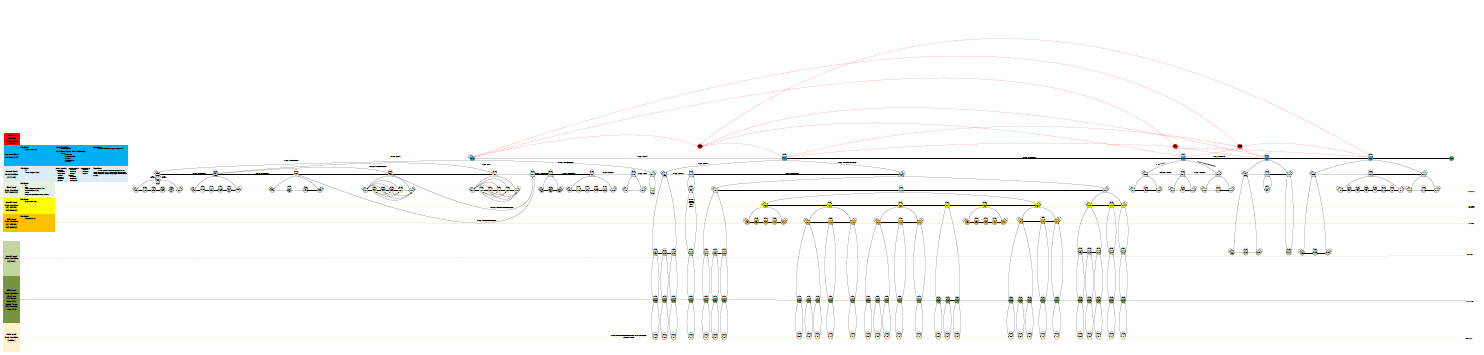
\includegraphics[scale=0.6]{appendix1.png}
\end{figure}\\
NOTE: A digital copy is available on the Syracuse University Google\textregistered
Drive in both pdf and visio formats. The visio formatted document contains
comments with descriptions, possible HOL implementation, and references
to the Ranger Handbook (where applicable).

\chapter{PB UML Class Diagram}
\label{cha:pb-uml-class}

\begin{figure}[h]
  \centering
  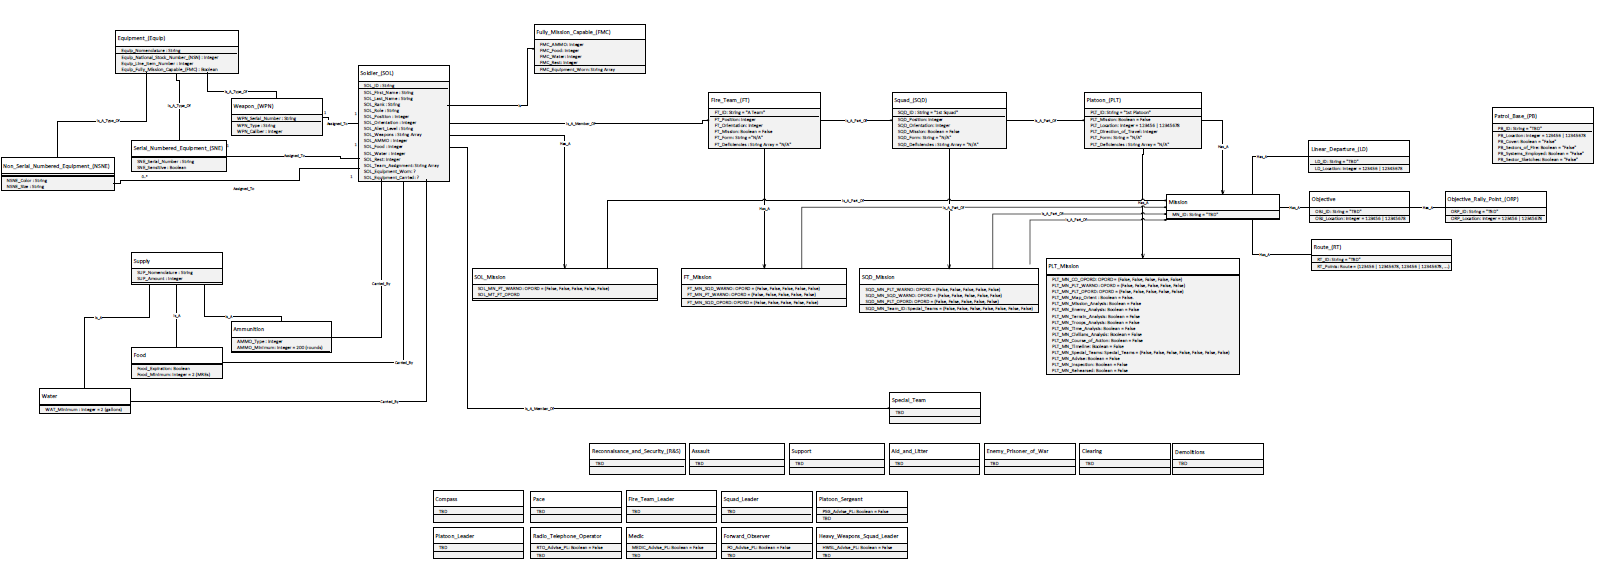
\includegraphics[scale=0.5]{appendix2.png}
\end{figure}\\
NOTE: A digital copy is available on the Syracuse University Google\textregistered
Drive in both pdf and visio formats. The visio formatted document contains
comments with descriptions, possible HOL implementation, and references
to the Ranger Handbook (where applicable).

\chapter{PLAN_PB DFD Level 0}
\label{cha:plan_pb-dfd-level}


\begin{figure}[h]
  \centering
  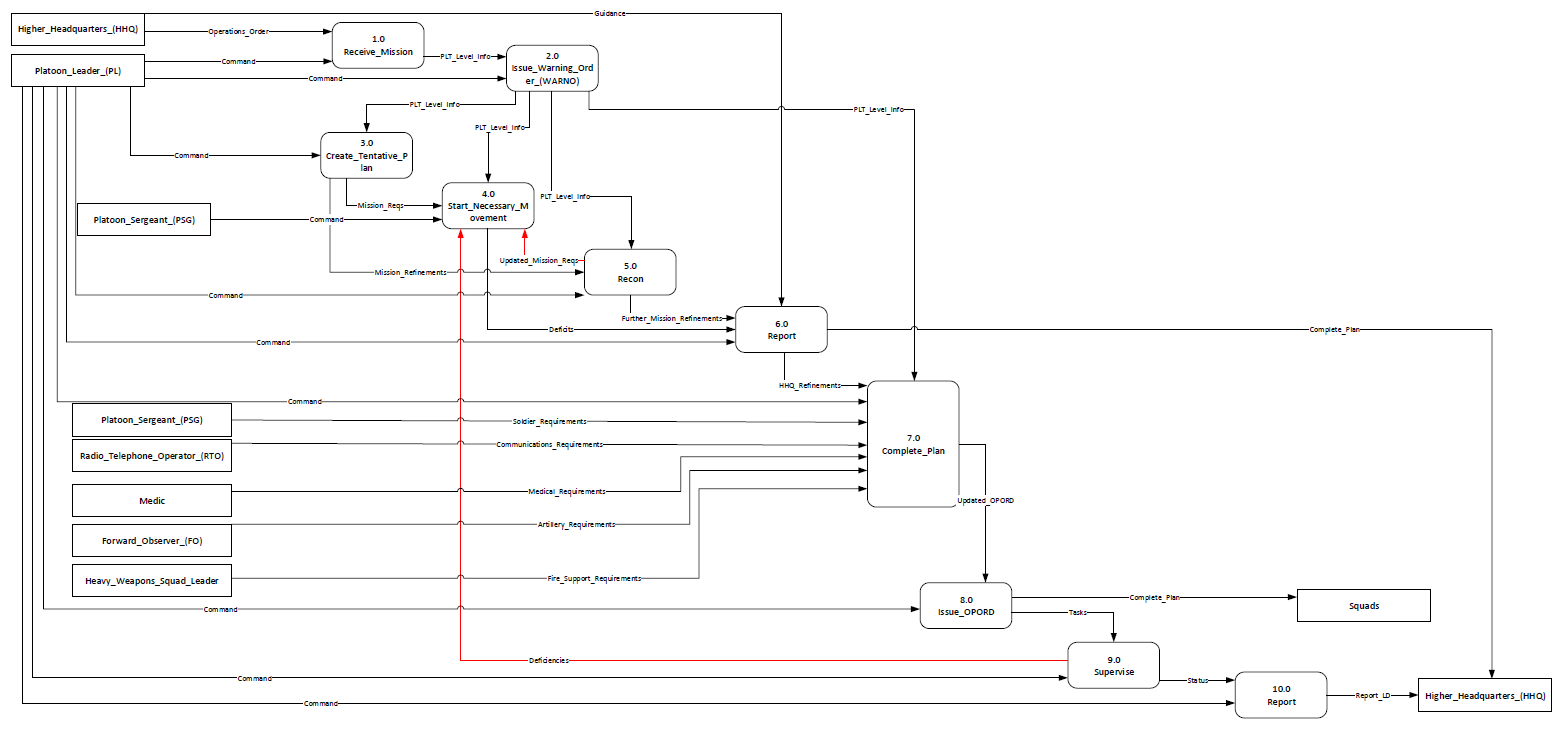
\includegraphics[scale=0.5]{appendix3.png}
\end{figure}\\
NOTE: A digital copy is available on the Syracuse University Google\textregistered
Drive in both pdf and visio formats. The visio formatted document contains
comments with descriptions, possible HOL implementation, and references
to the Ranger Handbook (where applicable).
\end{landscape}

\chapter{Next State, Next Output Table}
\label{cha:next-state-next}

\begin{table}[h!]
\begin{center}
  \resizebox{\textwidth}{!}{\begin{tabular}{|m{5em}|c|m{8em}|m{9em}|m{8em}|m{8em}|m{8em}|m{9em}|}
                              \hline
    \multicolumn{8}{|c|}{ }\\
    \multicolumn{8}{|c|}{\textcolor{cyan}{Next State}, Next Output Table}\\
    \multicolumn{8}{|c|}{ }\\
    \hline\hline
    & \cellcolor{cyan}State &&&&&&\\
    \hline
     \rowcolor{lime}Commands/ input &  \cellcolor{white}next state, next output  & crossLD & conductORP & moveToPB & conductPB & completePB & incomeplete \\
     \hline
     & \cellcolor{cyan}PLAN_PB & \textcolor{cyan}{MOVE_TO_ORP}, MoveToORP & \rowcolor{lightgray}  &  &&& \cellcolor{white}\textcolor{cyan}{PLAN_PB}, PlanPB \\
    \hline
     & \cellcolor{cyan}MOVE_TO_ORP & \rowcolor{lightgray}& \cellcolor{white}\textcolor{cyan}{CONDUCT_ORP}, ConductORP & & & & \cellcolor{white}\textcolor{cyan}{MOVE_TO_ORP}, MoveToORP \\
    \hline
     & \cellcolor{cyan}CONDUCT_ORP &\rowcolor{lightgray} & & \cellcolor{white}\textcolor{cyan}{MOVE_TO_PB}, MoveToPB & & & \cellcolor{white}\textcolor{cyan}{CONDUCT_ORP}, ConductORP \\
    \hline
     &\cellcolor{cyan} MOVE_TO_PB & \rowcolor{lightgray}&&& \cellcolor{white}\textcolor{cyan}{CONDUCT_PB}, ConductPB && \cellcolor{white}\textcolor{cyan}{MOVE_TO_PB}, MoveToPB \\
    \hline
     & \cellcolor{cyan}CONDUCT_PB & \rowcolor{lightgray}&&&& \cellcolor{white}\textcolor{cyan}{COMPLETE_PB}, CompletePB & \cellcolor{white}\textcolor{cyan}{CONDUCT_PB}, ConductPB \\
    \hline
     & \cellcolor{cyan}COMPLETE_PB & \rowcolor{lightgray} &&&&& \\
                              \hline

 \end{tabular}
 }
\end{center}
\end{table}

\chapter{Source code for ssmPBScript.sml}
\label{cha:source-code-ssmpbscr}

The following code is from \emph{ssmPBScript.sml}
\lstinputlisting{../HOL/ssmPB/ssmPBScript.sml}

\chapter{Source code for PBTypeScript.sml}
\label{cha:source-code-pbtyp}

The following code is from \emph{PBTypeScript.sml}
\lstinputlisting{../HOL/ssmPB/PBTypeScript.sml}

\chapter{Symbols, Abbreviations, and Acronyms}
\label{cha:list-symb-abbr}

\begin{align*}
&DFD\;\;\;\;\;&Data Flow Diagram\ \\
&HHQ\;\;\;\;\;&Higher Headquarters\ \\ 
&HOL\;\;\;\;\;&High Order Logic\ \\
&LD\;\;\;\;\;&Line of Departure/Linear Departure\ \\
&NMC\;\;\;\;\;&Non-Mission Capable\ \\
&OPORD\;\;\;\;\;&Operation Order\ \\
&PB\;\;\;\;\;&Patrol Base\ \\
&PL\;\;\;\;\;&Platoon Leader\ \\
&PolyML\;\;\;\;\;&Poly Metalanguage\ \\
&PSG\;\;\;\;\;&Platoon Sergeant\ \\
&TLP\;\;\;\;\;&Troop Leading Procedure\ \\
&UML\;\;\;\;\;&Unified Modeling Language\ \\
\end{align*}

\end{document}